% Options for packages loaded elsewhere
\PassOptionsToPackage{unicode}{hyperref}
\PassOptionsToPackage{hyphens}{url}
\PassOptionsToPackage{dvipsnames,svgnames*,x11names*}{xcolor}
%
\documentclass[
]{book}
\usepackage{lmodern}
\usepackage{amssymb,amsmath}
\usepackage{ifxetex,ifluatex}
\ifnum 0\ifxetex 1\fi\ifluatex 1\fi=0 % if pdftex
  \usepackage[T1]{fontenc}
  \usepackage[utf8]{inputenc}
  \usepackage{textcomp} % provide euro and other symbols
\else % if luatex or xetex
  \usepackage{unicode-math}
  \defaultfontfeatures{Scale=MatchLowercase}
  \defaultfontfeatures[\rmfamily]{Ligatures=TeX,Scale=1}
\fi
% Use upquote if available, for straight quotes in verbatim environments
\IfFileExists{upquote.sty}{\usepackage{upquote}}{}
\IfFileExists{microtype.sty}{% use microtype if available
  \usepackage[]{microtype}
  \UseMicrotypeSet[protrusion]{basicmath} % disable protrusion for tt fonts
}{}
\makeatletter
\@ifundefined{KOMAClassName}{% if non-KOMA class
  \IfFileExists{parskip.sty}{%
    \usepackage{parskip}
  }{% else
    \setlength{\parindent}{0pt}
    \setlength{\parskip}{6pt plus 2pt minus 1pt}}
}{% if KOMA class
  \KOMAoptions{parskip=half}}
\makeatother
\usepackage{xcolor}
\IfFileExists{xurl.sty}{\usepackage{xurl}}{} % add URL line breaks if available
\IfFileExists{bookmark.sty}{\usepackage{bookmark}}{\usepackage{hyperref}}
\hypersetup{
  pdftitle={Human-Plant Coevolution (HPC) model General exploration and parameter sensitivity analysis},
  colorlinks=true,
  linkcolor=Maroon,
  filecolor=Maroon,
  citecolor=Blue,
  urlcolor=blue,
  pdfcreator={LaTeX via pandoc}}
\urlstyle{same} % disable monospaced font for URLs
\usepackage{longtable,booktabs}
% Correct order of tables after \paragraph or \subparagraph
\usepackage{etoolbox}
\makeatletter
\patchcmd\longtable{\par}{\if@noskipsec\mbox{}\fi\par}{}{}
\makeatother
% Allow footnotes in longtable head/foot
\IfFileExists{footnotehyper.sty}{\usepackage{footnotehyper}}{\usepackage{footnote}}
\makesavenoteenv{longtable}
\usepackage{graphicx}
\makeatletter
\def\maxwidth{\ifdim\Gin@nat@width>\linewidth\linewidth\else\Gin@nat@width\fi}
\def\maxheight{\ifdim\Gin@nat@height>\textheight\textheight\else\Gin@nat@height\fi}
\makeatother
% Scale images if necessary, so that they will not overflow the page
% margins by default, and it is still possible to overwrite the defaults
% using explicit options in \includegraphics[width, height, ...]{}
\setkeys{Gin}{width=\maxwidth,height=\maxheight,keepaspectratio}
% Set default figure placement to htbp
\makeatletter
\def\fps@figure{htbp}
\makeatother
\setlength{\emergencystretch}{3em} % prevent overfull lines
\providecommand{\tightlist}{%
  \setlength{\itemsep}{0pt}\setlength{\parskip}{0pt}}
\setcounter{secnumdepth}{5}
\usepackage{fancyhdr}
\usepackage{placeins}
\usepackage{booktabs}
\usepackage{amsthm}
\makeatletter
\def\thm@space@setup{%
  \thm@preskip=8pt plus 2pt minus 4pt
  \thm@postskip=\thm@preskip
}
\makeatother

\title{Human-Plant Coevolution (HPC) modelGeneral exploration and parameter sensitivity analysis}
\author{}
\date{\vspace{-2.5em}2020-04-15}

\begin{document}
\maketitle

\newcommand{\HRule}{\rule{\linewidth}{0.5mm}}

\pagenumbering{gobble}

%\begin{titlepage}
\begin{center}

\textsc{\LARGE
\strong{H}uman-\strong{P}lant \strong{C}oevolution model} 
\\[1cm]
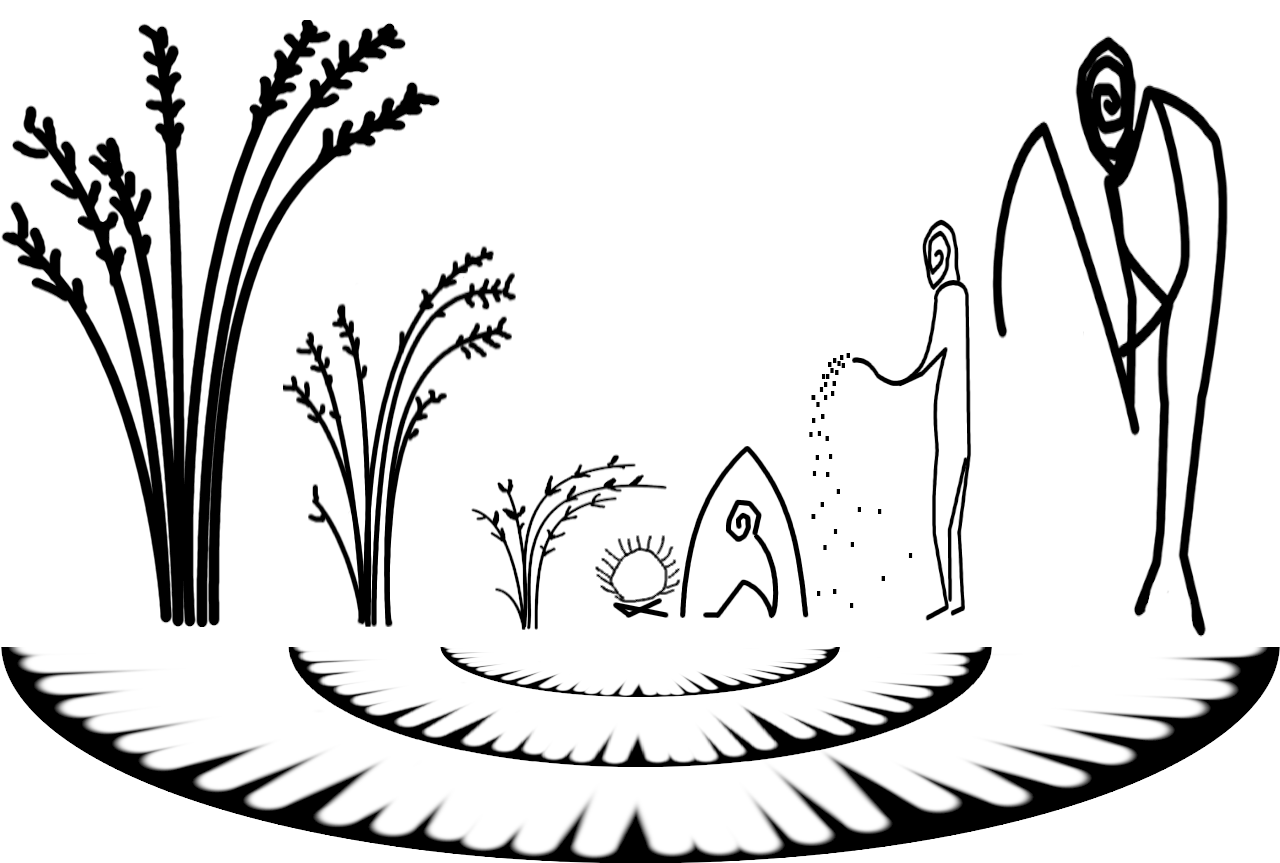
\includegraphics[width=\textwidth]{images/hpcModel-logo_v2.png}
\\[1.5cm]
\HRule \\[0.4cm]
{ \huge General exploration and parameter sensitivity analysis \\[0.15cm] }
\HRule \\[1.5cm]
Andreas Angourakis \& Jon\`{a}s Alcaina
\\[1cm]
\today \\ [1cm]

\end{center}
% \end{titlepage}

\newpage
\pagenumbering{arabic}

{
\hypersetup{linkcolor=}
\setcounter{tocdepth}{1}
\tableofcontents
}
\hypertarget{section}{%
\chapter*{\_\_\_\_\_\_\_}\label{section}}
\addcontentsline{toc}{chapter}{\_\_\_\_\_\_\_}

\hypertarget{model-overview}{%
\chapter*{Model overview}\label{model-overview}}
\addcontentsline{toc}{chapter}{Model overview}

The Human-Plant Coevolution (HPC) model represents the dynamics of coevolution between a human and a plant population. The model consists of an ecological positive feedback system (mutualism), which can be reinforced by positive evolutionary feedback (coevolution). The model is the result of wiring together relatively simple simulation models of population ecology and evolution, through a computational implementation in R.

\newpage

\textbf{\emph{Parameters}}

\begin{longtable}[]{@{}lll@{}}
\caption{Parameters}\tabularnewline
\toprule
\begin{minipage}[b]{0.27\columnwidth}\raggedright
R notation\strut
\end{minipage} & \begin{minipage}[b]{0.25\columnwidth}\raggedright
Math notation\strut
\end{minipage} & \begin{minipage}[b]{0.40\columnwidth}\raggedright
Description\strut
\end{minipage}\tabularnewline
\midrule
\endfirsthead
\toprule
\begin{minipage}[b]{0.27\columnwidth}\raggedright
R notation\strut
\end{minipage} & \begin{minipage}[b]{0.25\columnwidth}\raggedright
Math notation\strut
\end{minipage} & \begin{minipage}[b]{0.40\columnwidth}\raggedright
Description\strut
\end{minipage}\tabularnewline
\midrule
\endhead
\begin{minipage}[t]{0.27\columnwidth}\raggedright
\texttt{iniH}, \texttt{iniP}\strut
\end{minipage} & \begin{minipage}[t]{0.25\columnwidth}\raggedright
\(ini_{H},\,ini_{P}\)\strut
\end{minipage} & \begin{minipage}[t]{0.40\columnwidth}\raggedright
\textbf{initial populations of humans and plants}\strut
\end{minipage}\tabularnewline
\begin{minipage}[t]{0.27\columnwidth}\raggedright
\texttt{n.H}, \texttt{n.P}\strut
\end{minipage} & \begin{minipage}[t]{0.25\columnwidth}\raggedright
\(n_{H},\,n_{P}\)\strut
\end{minipage} & \begin{minipage}[t]{0.40\columnwidth}\raggedright
\textbf{number of types of humans and plants}. The number of phenotypic variants of each population that relate to human-plant coevolution. Types are arbitrarily ordered from type \(1\) (\emph{less} mutualistic) to type \(n\) (\emph{more} mutualistic).\strut
\end{minipage}\tabularnewline
\begin{minipage}[t]{0.27\columnwidth}\raggedright
\texttt{v.H}, \texttt{v.P}\strut
\end{minipage} & \begin{minipage}[t]{0.25\columnwidth}\raggedright
\(v_{H},\,v_{P}\)\strut
\end{minipage} & \begin{minipage}[t]{0.40\columnwidth}\raggedright
\textbf{level of undirected variation in humans and plants}. For any value greater than zero, these parameters regulate how even is the distribution of a population among its types.\strut
\end{minipage}\tabularnewline
\begin{minipage}[t]{0.27\columnwidth}\raggedright
\texttt{r.H}, \texttt{r.P}\strut
\end{minipage} & \begin{minipage}[t]{0.25\columnwidth}\raggedright
\(r_{H},\,r_{P}\)\strut
\end{minipage} & \begin{minipage}[t]{0.40\columnwidth}\raggedright
\textbf{intrinsic growth rates for human and plant populations}. The maximum rate at which a population grows when there are no external constraints.\strut
\end{minipage}\tabularnewline
\begin{minipage}[t]{0.27\columnwidth}\raggedright
\texttt{mU.PnH}\strut
\end{minipage} & \begin{minipage}[t]{0.25\columnwidth}\raggedright
\(\bar{U}_{P_{n}H}\)\strut
\end{minipage} & \begin{minipage}[t]{0.40\columnwidth}\raggedright
utility per capita of \textbf{type} \(n\) \textbf{plants} to \textbf{humans}\strut
\end{minipage}\tabularnewline
\begin{minipage}[t]{0.27\columnwidth}\raggedright
\texttt{mU.HnP}\strut
\end{minipage} & \begin{minipage}[t]{0.25\columnwidth}\raggedright
\(\bar{U}_{H_{n}P}\)\strut
\end{minipage} & \begin{minipage}[t]{0.40\columnwidth}\raggedright
utility per capita of \textbf{type} \(n\) \textbf{humans} to \textbf{plants}\strut
\end{minipage}\tabularnewline
\begin{minipage}[t]{0.27\columnwidth}\raggedright
\texttt{mU.P1H}\strut
\end{minipage} & \begin{minipage}[t]{0.25\columnwidth}\raggedright
\(\bar{U}_{P_{1}H}\)\strut
\end{minipage} & \begin{minipage}[t]{0.40\columnwidth}\raggedright
utility per capita of \textbf{type} \(1\) \textbf{plants} to \textbf{humans}\strut
\end{minipage}\tabularnewline
\begin{minipage}[t]{0.27\columnwidth}\raggedright
\texttt{mU.H1P}\strut
\end{minipage} & \begin{minipage}[t]{0.25\columnwidth}\raggedright
\(\bar{U}_{H_{1}P}\)\strut
\end{minipage} & \begin{minipage}[t]{0.40\columnwidth}\raggedright
utility per capita of \textbf{type} \(1\) \textbf{humans} to \textbf{plants}\strut
\end{minipage}\tabularnewline
\begin{minipage}[t]{0.27\columnwidth}\raggedright
\texttt{U.bH1}\strut
\end{minipage} & \begin{minipage}[t]{0.25\columnwidth}\raggedright
\(U_{bH_{1}}\)\strut
\end{minipage} & \begin{minipage}[t]{0.40\columnwidth}\raggedright
utility of \textbf{other resources} to \textbf{type} \(1\) \textbf{humans} or the baseline carrying capacity for humans of type \(1\); i.e.~that independent of plants.\strut
\end{minipage}\tabularnewline
\begin{minipage}[t]{0.27\columnwidth}\raggedright
\texttt{U.bP1}\strut
\end{minipage} & \begin{minipage}[t]{0.25\columnwidth}\raggedright
\(U_{bP_{1}}\)\strut
\end{minipage} & \begin{minipage}[t]{0.40\columnwidth}\raggedright
utility of \textbf{other resources} to \textbf{type} \(1\) \textbf{plants} or the baseline carrying capacity for plants of type \(1\); i.e.~that independent of humans. (non-anthropic space)\strut
\end{minipage}\tabularnewline
\begin{minipage}[t]{0.27\columnwidth}\raggedright
\texttt{U.bHn}\strut
\end{minipage} & \begin{minipage}[t]{0.25\columnwidth}\raggedright
\(U_{bH_{n}}\)\strut
\end{minipage} & \begin{minipage}[t]{0.40\columnwidth}\raggedright
utility of \textbf{other resources} to \textbf{type} \(n\) \textbf{humans} or the baseline carrying capacity for humans of type \(n\), i.e.~that independent of plants\strut
\end{minipage}\tabularnewline
\begin{minipage}[t]{0.27\columnwidth}\raggedright
\texttt{U.bPn}\strut
\end{minipage} & \begin{minipage}[t]{0.25\columnwidth}\raggedright
\(U_{bP_{n}}\)\strut
\end{minipage} & \begin{minipage}[t]{0.40\columnwidth}\raggedright
utility of \textbf{other resources} to \textbf{type} \(n\) \textbf{plants} or the baseline carrying capacity for plants of type \(n\); i.e.~that independent of humans.\strut
\end{minipage}\tabularnewline
\begin{minipage}[t]{0.27\columnwidth}\raggedright
\texttt{MaxArea}\strut
\end{minipage} & \begin{minipage}[t]{0.25\columnwidth}\raggedright
\(MaxArea\)\strut
\end{minipage} & \begin{minipage}[t]{0.40\columnwidth}\raggedright
\textbf{Maximum number of plant population units fitting the contiguous area available}. It is used as the maximum carrying capacity for plants.\strut
\end{minipage}\tabularnewline
\bottomrule
\end{longtable}

\newpage

\begin{longtable}[]{@{}lll@{}}
\caption{Variables}\tabularnewline
\toprule
\begin{minipage}[b]{0.36\columnwidth}\raggedright
R notation\strut
\end{minipage} & \begin{minipage}[b]{0.21\columnwidth}\raggedright
Math notation\strut
\end{minipage} & \begin{minipage}[b]{0.34\columnwidth}\raggedright
Description\strut
\end{minipage}\tabularnewline
\midrule
\endfirsthead
\toprule
\begin{minipage}[b]{0.36\columnwidth}\raggedright
R notation\strut
\end{minipage} & \begin{minipage}[b]{0.21\columnwidth}\raggedright
Math notation\strut
\end{minipage} & \begin{minipage}[b]{0.34\columnwidth}\raggedright
Description\strut
\end{minipage}\tabularnewline
\midrule
\endhead
\begin{minipage}[t]{0.36\columnwidth}\raggedright
\texttt{H}, \texttt{P}\strut
\end{minipage} & \begin{minipage}[t]{0.21\columnwidth}\raggedright
\(H[t],\,P[t]\)\strut
\end{minipage} & \begin{minipage}[t]{0.34\columnwidth}\raggedright
\textbf{Human and plant populations} at time \(t\). Population units are abstract, arbitrarily defined units that can express individuals, working hours, households, etc. (humans), and sprouts, certain amount of biomass, soil surface, etc. (plants)\strut
\end{minipage}\tabularnewline
\begin{minipage}[t]{0.36\columnwidth}\raggedright
\texttt{K.H}, \texttt{K.P}\strut
\end{minipage} & \begin{minipage}[t]{0.21\columnwidth}\raggedright
\(K_{H}[t],\,K_{P}[t]\)\strut
\end{minipage} & \begin{minipage}[t]{0.34\columnwidth}\raggedright
\textbf{Carrying capacity} to human and plant populations or maximum population at time \(t\), expressed in population units\strut
\end{minipage}\tabularnewline
\begin{minipage}[t]{0.36\columnwidth}\raggedright
\texttt{U.HP}, \texttt{U.PH}\strut
\end{minipage} & \begin{minipage}[t]{0.21\columnwidth}\raggedright
\(U_{HP}[t],\,U_{PH}[t]\)\strut
\end{minipage} & \begin{minipage}[t]{0.34\columnwidth}\raggedright
\textbf{Utility of one population to the other} or the total contribution of a population to the carrying capacity of the other population at time \(t\), expressed in population units\strut
\end{minipage}\tabularnewline
\begin{minipage}[t]{0.36\columnwidth}\raggedright
\texttt{U.bH}, \texttt{U.bP}\strut
\end{minipage} & \begin{minipage}[t]{0.21\columnwidth}\raggedright
\(U_{bH}[t],\,U_{bP}[t]\)\strut
\end{minipage} & \begin{minipage}[t]{0.34\columnwidth}\raggedright
\textbf{Utility of other resources to a population} at time \(t\), expressed in population units (baseline carrying capacity)\strut
\end{minipage}\tabularnewline
\begin{minipage}[t]{0.36\columnwidth}\raggedright
\texttt{types.H}, \texttt{types.P}\strut
\end{minipage} & \begin{minipage}[t]{0.21\columnwidth}\raggedright
\(types_{H},\,types_{P}\)\strut
\end{minipage} & \begin{minipage}[t]{0.34\columnwidth}\raggedright
Population types, arbitrarily ordered from \(1\) to \(n\) (vector or array).\strut
\end{minipage}\tabularnewline
\begin{minipage}[t]{0.36\columnwidth}\raggedright
\texttt{pop.H}, \texttt{pop.P}\strut
\end{minipage} & \begin{minipage}[t]{0.21\columnwidth}\raggedright
\(pop_{H_{i}}[t],\,pop_{P_{i}}[t]\)\strut
\end{minipage} & \begin{minipage}[t]{0.34\columnwidth}\raggedright
\textbf{Proportion of a population} belonging to type \(i\) at time \(t\) (vector or array).\strut
\end{minipage}\tabularnewline
\begin{minipage}[t]{0.36\columnwidth}\raggedright
\texttt{mU.HP.per.type}, \texttt{mU.PH.per.type}\strut
\end{minipage} & \begin{minipage}[t]{0.21\columnwidth}\raggedright
\(\bar{U}_{H_{i}P},\,\bar{U}_{P_{i}H}\)\strut
\end{minipage} & \begin{minipage}[t]{0.34\columnwidth}\raggedright
\textbf{Utility per capita} of type \(i\) individuals of one population to the other (vector or array).\strut
\end{minipage}\tabularnewline
\begin{minipage}[t]{0.36\columnwidth}\raggedright
\texttt{U.bH.per.type}, \texttt{U.bP.per.type}\strut
\end{minipage} & \begin{minipage}[t]{0.21\columnwidth}\raggedright
\(U_{bH_{i}},\,U_{bP_{i}}\)\strut
\end{minipage} & \begin{minipage}[t]{0.34\columnwidth}\raggedright
\textbf{Utility of other resources} to type \(i\) individuals of a population (vector or array).\strut
\end{minipage}\tabularnewline
\begin{minipage}[t]{0.36\columnwidth}\raggedright
\texttt{fitness.H}, \texttt{fitness.P}\strut
\end{minipage} & \begin{minipage}[t]{0.21\columnwidth}\raggedright
\(fitness_{H_{i}}[t]\), \(fitness_{P_{i}}[t]\)\strut
\end{minipage} & \begin{minipage}[t]{0.34\columnwidth}\raggedright
\textbf{Fitness score} of type \(i\) individuals of a population at time \(t\) (vector or array).\strut
\end{minipage}\tabularnewline
\begin{minipage}[t]{0.36\columnwidth}\raggedright
\texttt{d.H}, \texttt{d.P}\strut
\end{minipage} & \begin{minipage}[t]{0.21\columnwidth}\raggedright
\(\Delta H[t],\,\Delta P[t]\)\strut
\end{minipage} & \begin{minipage}[t]{0.34\columnwidth}\raggedright
\textbf{Population change} (\emph{delta}) at time \(t\) in respect to time \(t -1\) (vector or array).\strut
\end{minipage}\tabularnewline
\bottomrule
\end{longtable}

\newpage

\begin{longtable}[]{@{}lll@{}}
\caption{Variables (output only)}\tabularnewline
\toprule
\begin{minipage}[b]{0.36\columnwidth}\raggedright
R notation\strut
\end{minipage} & \begin{minipage}[b]{0.21\columnwidth}\raggedright
Math notation\strut
\end{minipage} & \begin{minipage}[b]{0.34\columnwidth}\raggedright
Description\strut
\end{minipage}\tabularnewline
\midrule
\endfirsthead
\toprule
\begin{minipage}[b]{0.36\columnwidth}\raggedright
R notation\strut
\end{minipage} & \begin{minipage}[b]{0.21\columnwidth}\raggedright
Math notation\strut
\end{minipage} & \begin{minipage}[b]{0.34\columnwidth}\raggedright
Description\strut
\end{minipage}\tabularnewline
\midrule
\endhead
\begin{minipage}[t]{0.36\columnwidth}\raggedright
\texttt{coevo.H}, \texttt{coevo.P}\strut
\end{minipage} & \begin{minipage}[t]{0.21\columnwidth}\raggedright
\(coevo_{H},\,coevo_{P}\)\strut
\end{minipage} & \begin{minipage}[t]{0.34\columnwidth}\raggedright
\textbf{Coevolution coefficients}. A coefficient representing the distribution of the proportion of a population per type (\(pop_{A_1}\) to \(pop_{A_n}\)) weighted by type index (\(1\) to \(n\)). Each indicates \emph{if} and \emph{how much} the population distribution has been modified by the coevolutionary process. Their values range between -1, the entire population is of type \(1\), and 1, the entire population is of type \(n\).\strut
\end{minipage}\tabularnewline
\begin{minipage}[t]{0.36\columnwidth}\raggedright
\texttt{depend.H}, \texttt{depend.P}\strut
\end{minipage} & \begin{minipage}[t]{0.21\columnwidth}\raggedright
\(depend_{H},\,depend_{P}\)\strut
\end{minipage} & \begin{minipage}[t]{0.34\columnwidth}\raggedright
\textbf{Dependency coefficients}. The slope of the linear model of the fitness score per type (\(fitness_{A_1}\) to \(fitness_{A_n}\)) using type index (\(1\) to \(n\)). Indicate \emph{if} and \emph{how much} the overall fitness score of a population is dependent on the other population.\strut
\end{minipage}\tabularnewline
\begin{minipage}[t]{0.36\columnwidth}\raggedright
\texttt{timing.H}, \texttt{timing.P}\strut
\end{minipage} & \begin{minipage}[t]{0.21\columnwidth}\raggedright
\(timing_{H},\,timing_{P}\)\strut
\end{minipage} & \begin{minipage}[t]{0.34\columnwidth}\raggedright
\textbf{Iterations past} until \textbf{coevolution} successfully changes the proportions of population per type; generally, when \(pop_{A_1}\gg pop_{A_n}\) or, more specifically, \(coevo_A>timing.threshold\).\strut
\end{minipage}\tabularnewline
\begin{minipage}[t]{0.36\columnwidth}\raggedright
\texttt{time}\strut
\end{minipage} & \begin{minipage}[t]{0.21\columnwidth}\raggedright
\(t_{end}\)\strut
\end{minipage} & \begin{minipage}[t]{0.34\columnwidth}\raggedright
\textbf{Iterations past} until the \textbf{end state} (\emph{stationary point})\strut
\end{minipage}\tabularnewline
\bottomrule
\end{longtable}

\hypertarget{single-runs}{%
\chapter{Single runs}\label{single-runs}}

Attractors are system stable states, in which all variables become, at some level, predictable (i.e., they attract trajectories). For most of the conditions explored, the HPC model displays stationary points, which are attractors where variables converge and do not change unless the system is perturbed.

Another kind of attractor, oscillations, exists. A special case of oscillation occurs when either the iteration unit or at least one of the intrinsic growth rates are greater than the unit ( dt \textgreater{} 1 or rA \textgreater{} 1 ). Such behaviour is a common feature of logistic growth models and was already observed and analysed by Hastings (1997). More interestingly, certain, less extreme parameter configurations also produce oscillatory states (see last section in this chapter).

\newpage

\hypertarget{fast-coevolution-default}{%
\section{Fast coevolution (default)}\label{fast-coevolution-default}}

\begin{table}[!h]

\caption{\label{tab:1runcoevocoetaparspdf}Parameter setting}
\centering
\begin{tabular}[t]{l|l}
\hline
parameter & values\\
\hline
iniH & 10\\
\hline
iniP & 10\\
\hline
n.H & 30\\
\hline
n.P & 30\\
\hline
v.H & 0.15\\
\hline
v.P & 0.15\\
\hline
r.H & 0.04\\
\hline
r.P & 0.1\\
\hline
mU.PnH & 1.5\\
\hline
mU.HnP & 1\\
\hline
mU.P1H & 0.15\\
\hline
mU.H1P & 0\\
\hline
U.bHn & 10\\
\hline
U.bPn & 20\\
\hline
U.bH1 & 80\\
\hline
U.bP1 & 100\\
\hline
MaxArea & 200\\
\hline
maxIt & 5000\\
\hline
tol & 6\\
\hline
timing.threshold & 0.5\\
\hline
\end{tabular}
\end{table}

\vspace{1cm}

\begin{longtable}[]{@{}ll@{}}
\caption{Output variables (values at end state)}\tabularnewline
\toprule
Abbreviation & Value\tabularnewline
\midrule
\endfirsthead
\toprule
Abbreviation & Value\tabularnewline
\midrule
\endhead
\texttt{time} & 699\tabularnewline
\texttt{coevo.H} & 0.6913054\tabularnewline
\texttt{coevo.P} & 0.6763894\tabularnewline
\texttt{depend.H} & 0.8855591\tabularnewline
\texttt{depend.P} & 0.8058295\tabularnewline
\texttt{timing.H} & 236\tabularnewline
\texttt{timing.P} & 252\tabularnewline
\bottomrule
\end{longtable}

\newpage

\begin{figure}
\centering
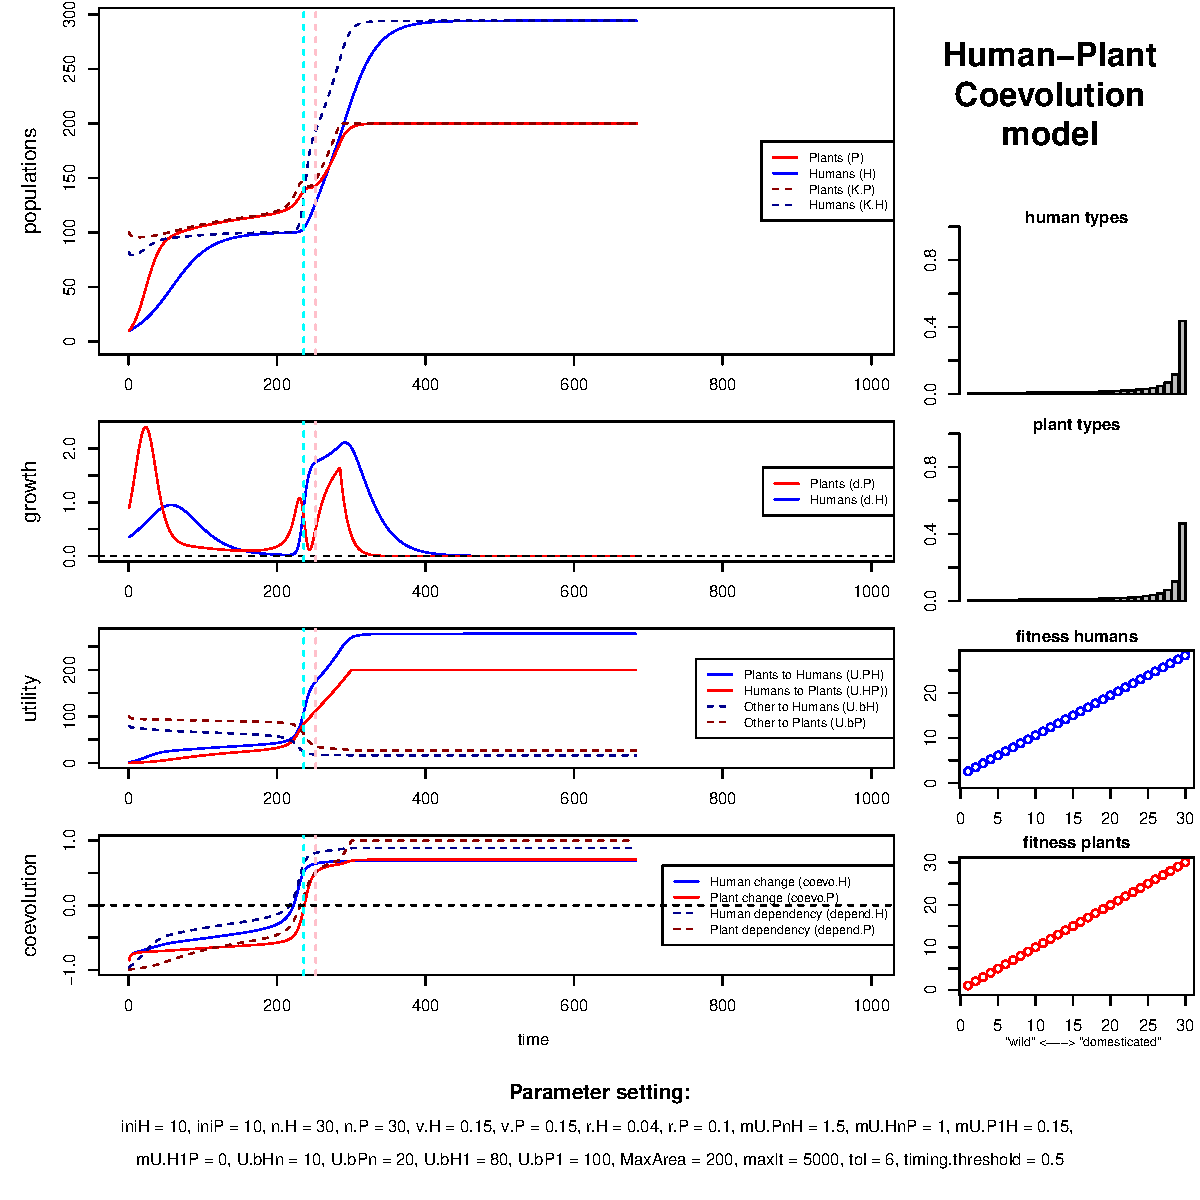
\includegraphics{hpcModel-exploration_files/figure-latex/1runcoevocoetaplot-1.pdf}
\caption{\label{fig:1runcoevocoetaplot}Plotting the end state, i.e.~both populations become stationary}
\end{figure}

\newpage

\begin{figure}
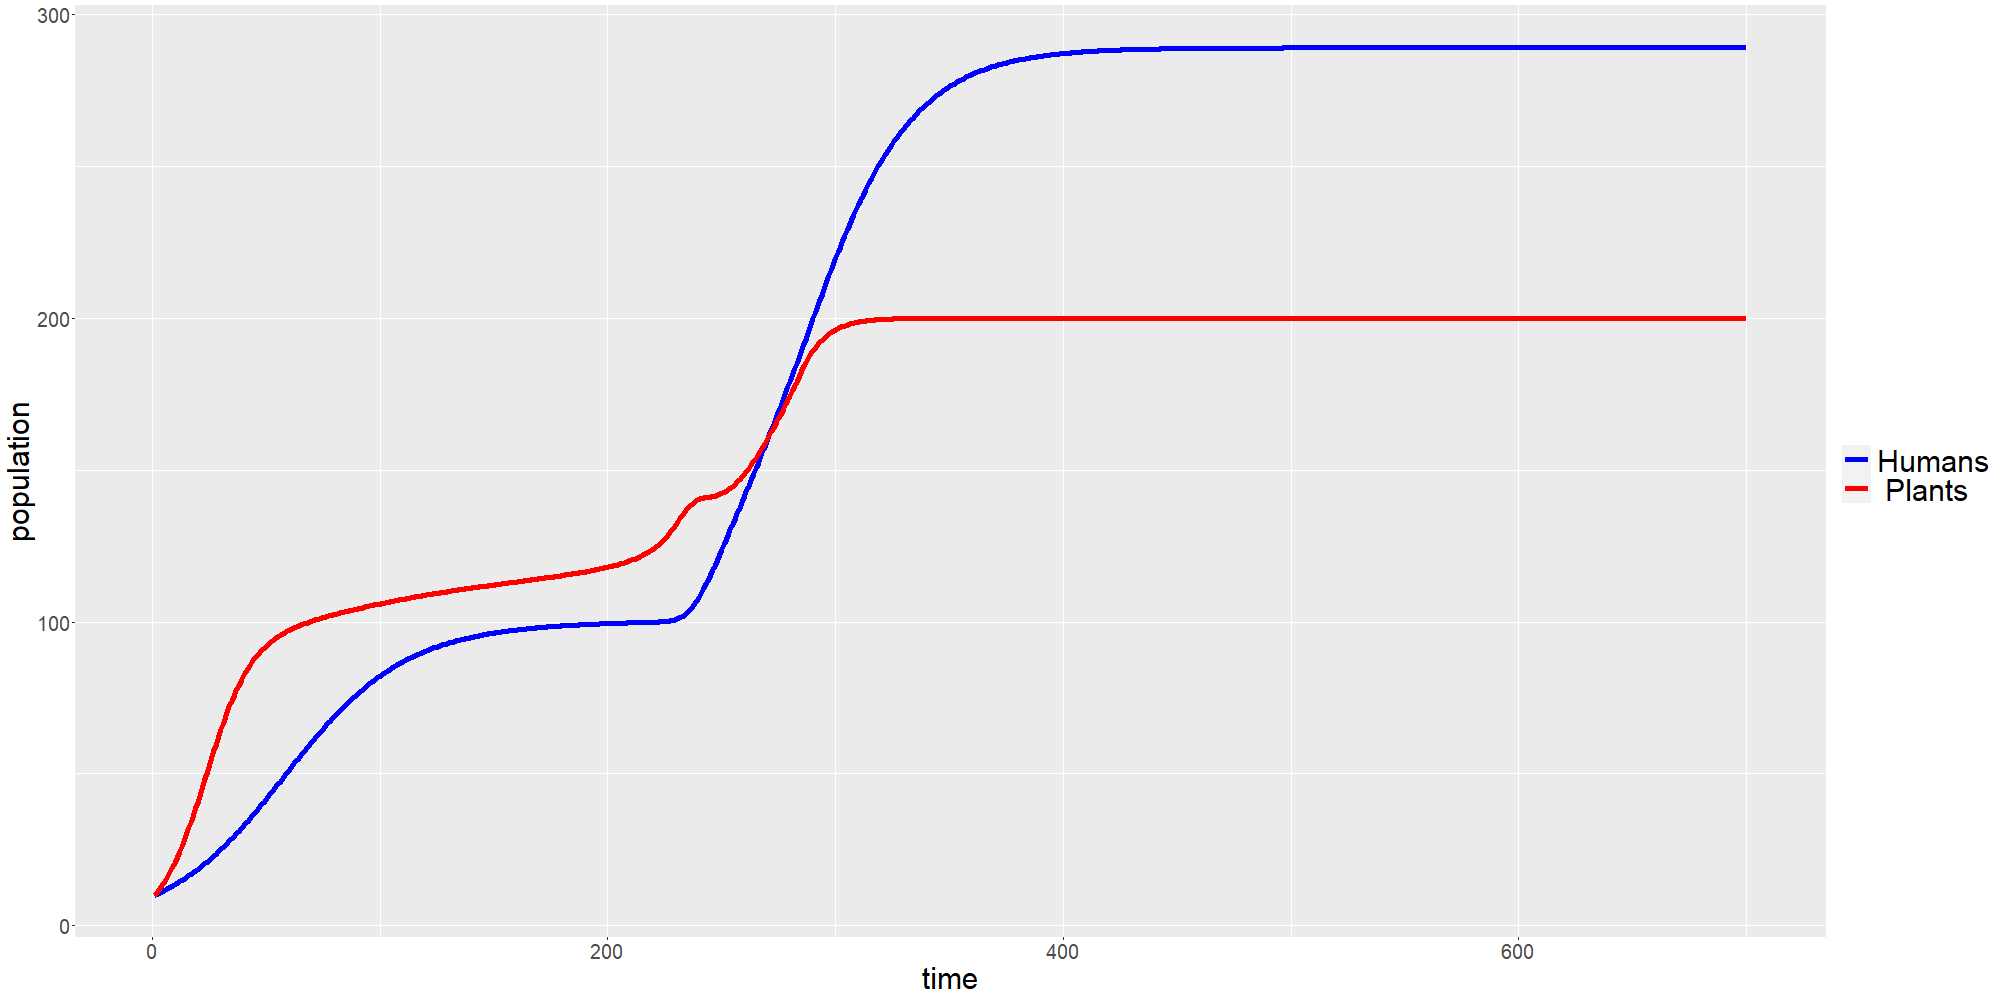
\includegraphics[width=1\linewidth]{plots/1_singleRun-ggplot-run.coevo.coeta} \caption{Plotting population trajectories with ggplot2}\label{fig:1runcoevocoetaggplotprint}
\end{figure}

\newpage

\FloatBarrier
\newpage

\hypertarget{no-coevolution}{%
\section{No coevolution}\label{no-coevolution}}

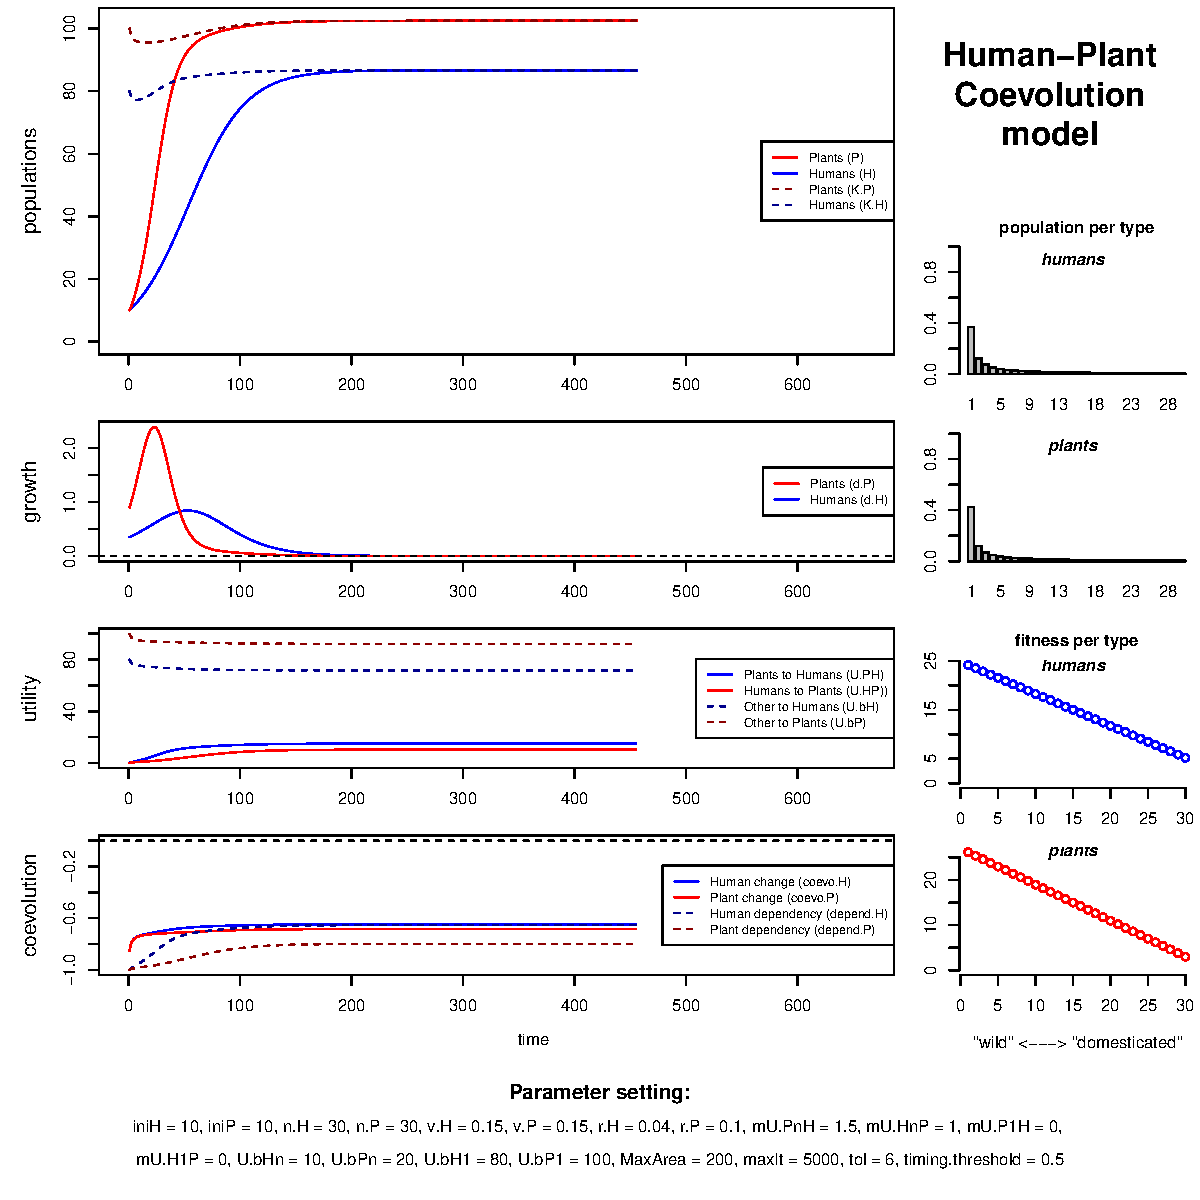
\includegraphics{hpcModel-exploration_files/figure-latex/1_run.no.coevo-plot-1.pdf}

\newpage

\hypertarget{coevolution-with-early-cultivation}{%
\section{Coevolution with early cultivation}\label{coevolution-with-early-cultivation}}

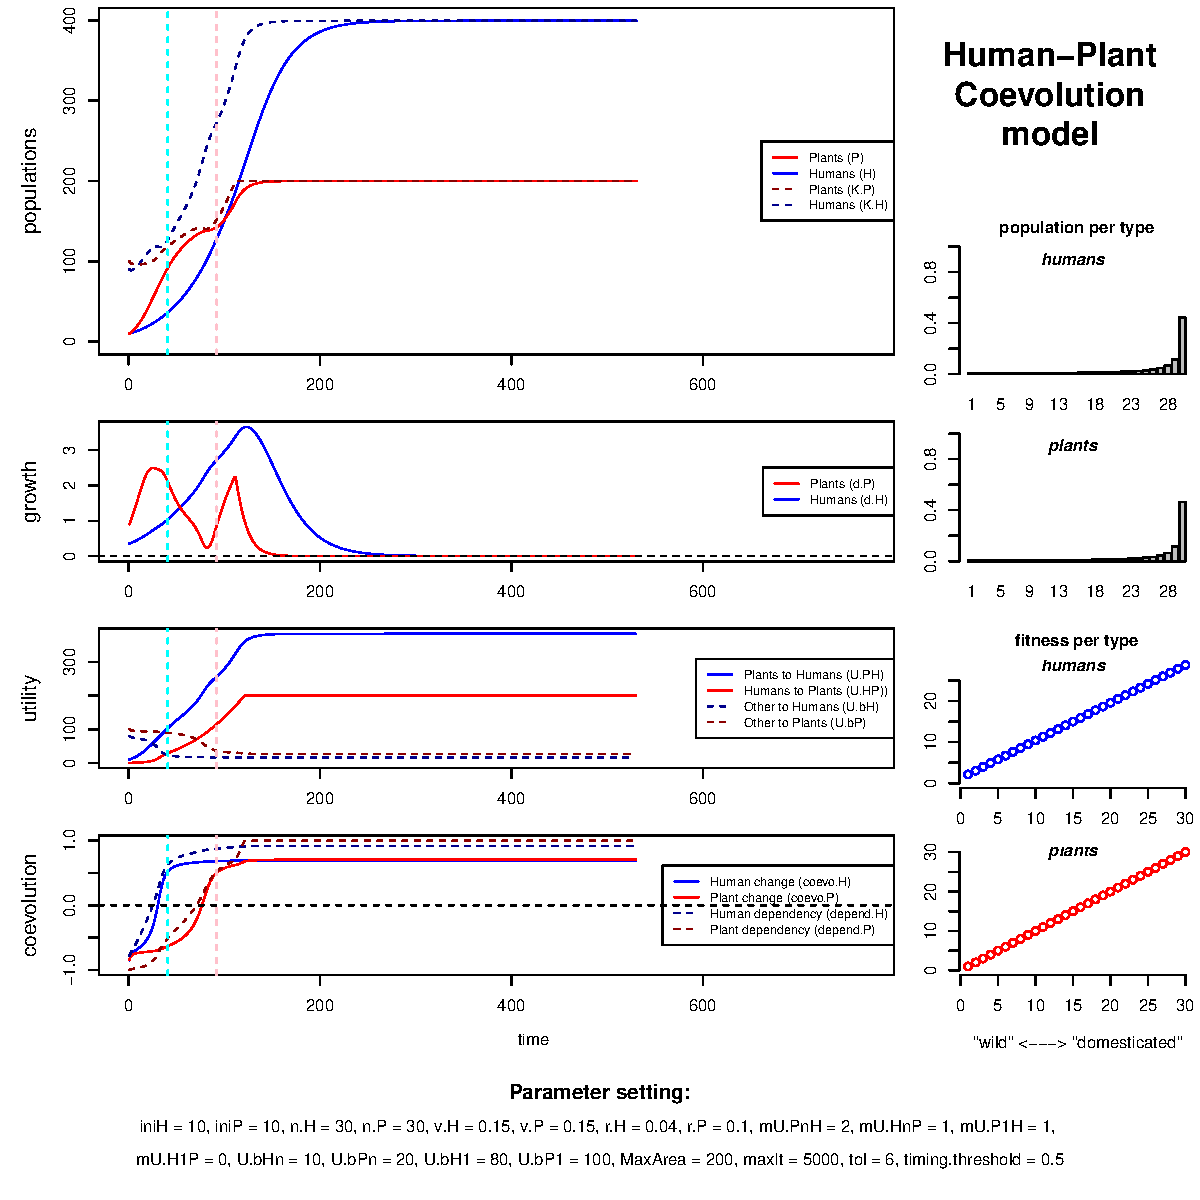
\includegraphics{hpcModel-exploration_files/figure-latex/1_run.coevo.early.cult-plot-1.pdf}

\newpage

\hypertarget{coevolution-with-early-domestication}{%
\section{Coevolution with early domestication}\label{coevolution-with-early-domestication}}

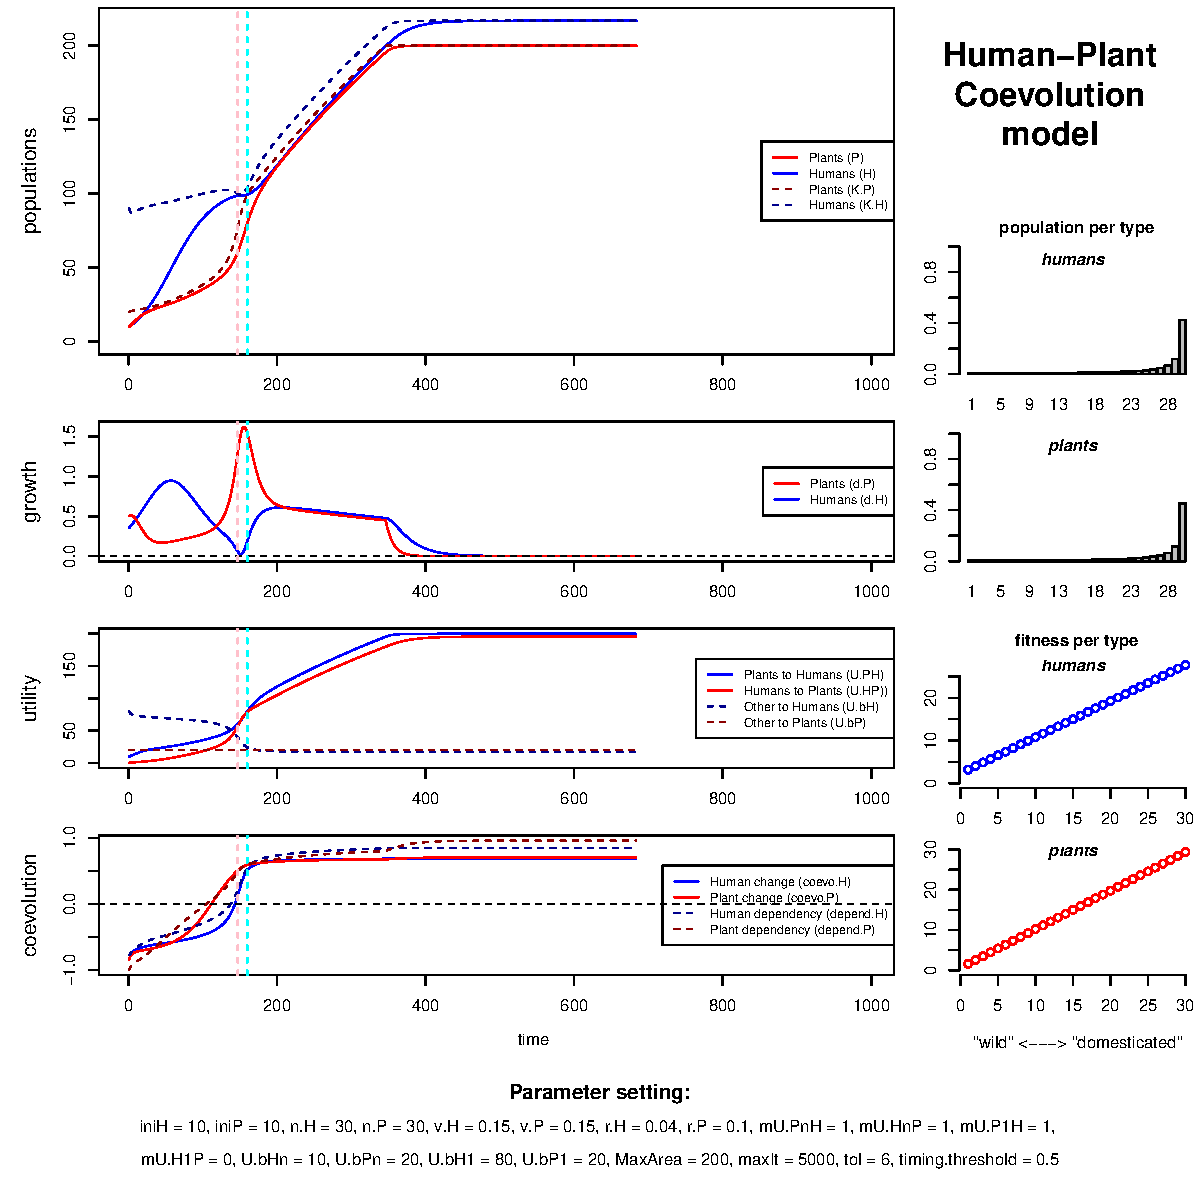
\includegraphics{hpcModel-exploration_files/figure-latex/1_run.coevo.early.dom-plot-1.pdf}

\newpage

\hypertarget{cultivation-without-domestication}{%
\section{Cultivation without domestication}\label{cultivation-without-domestication}}

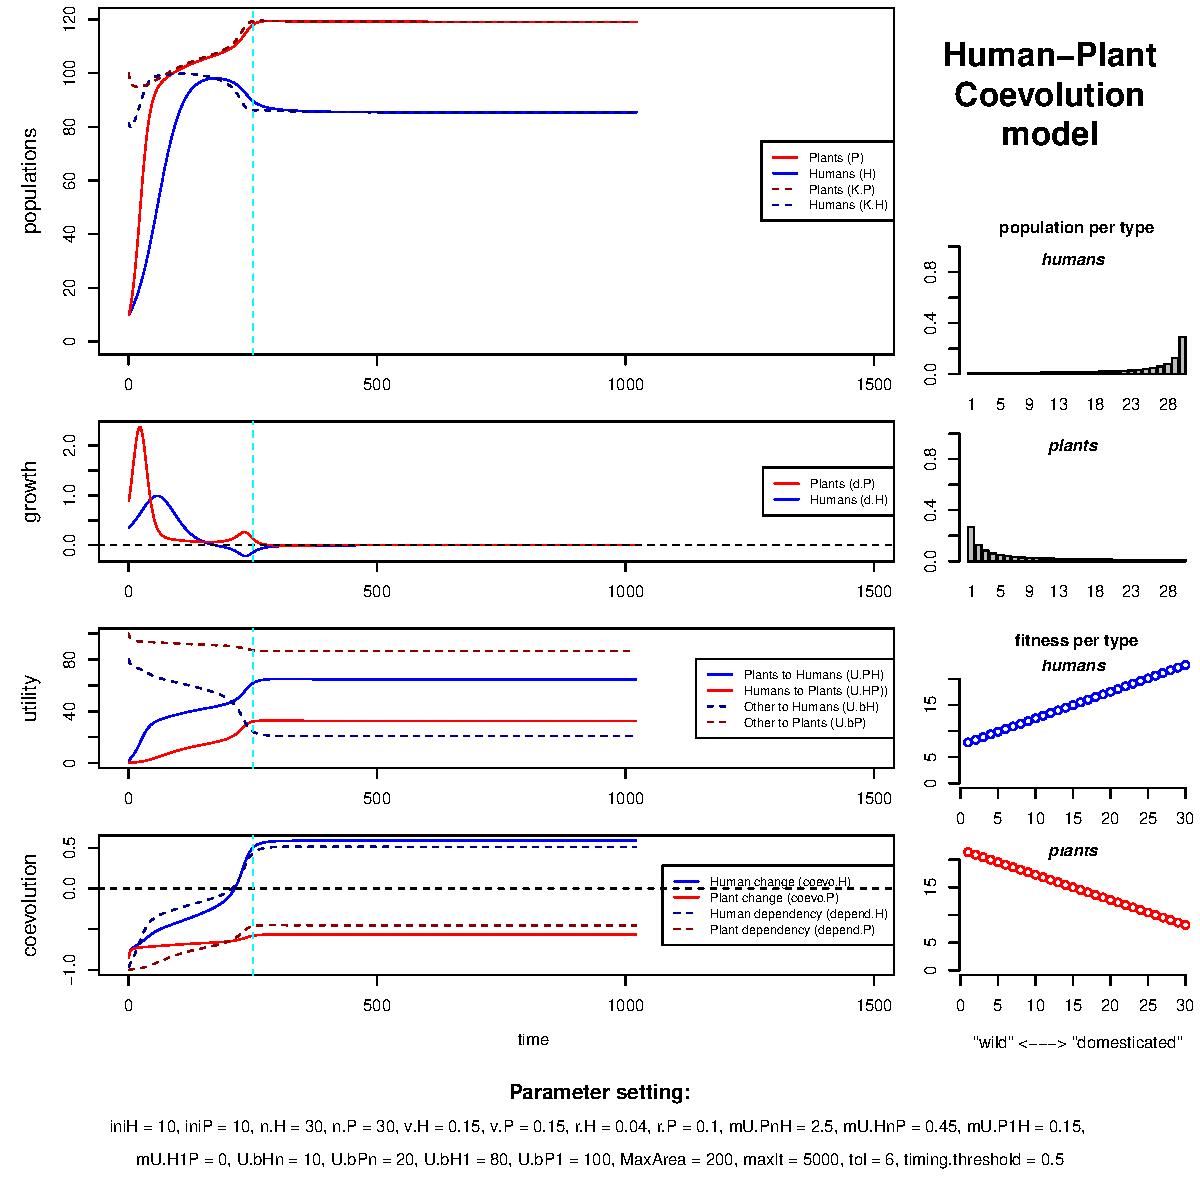
\includegraphics{hpcModel-exploration_files/figure-latex/1_run.cult.without.dom-plot-1.pdf}

\newpage

\hypertarget{coevolution-with-population-bleep}{%
\section{Coevolution with population ``bleep''}\label{coevolution-with-population-bleep}}

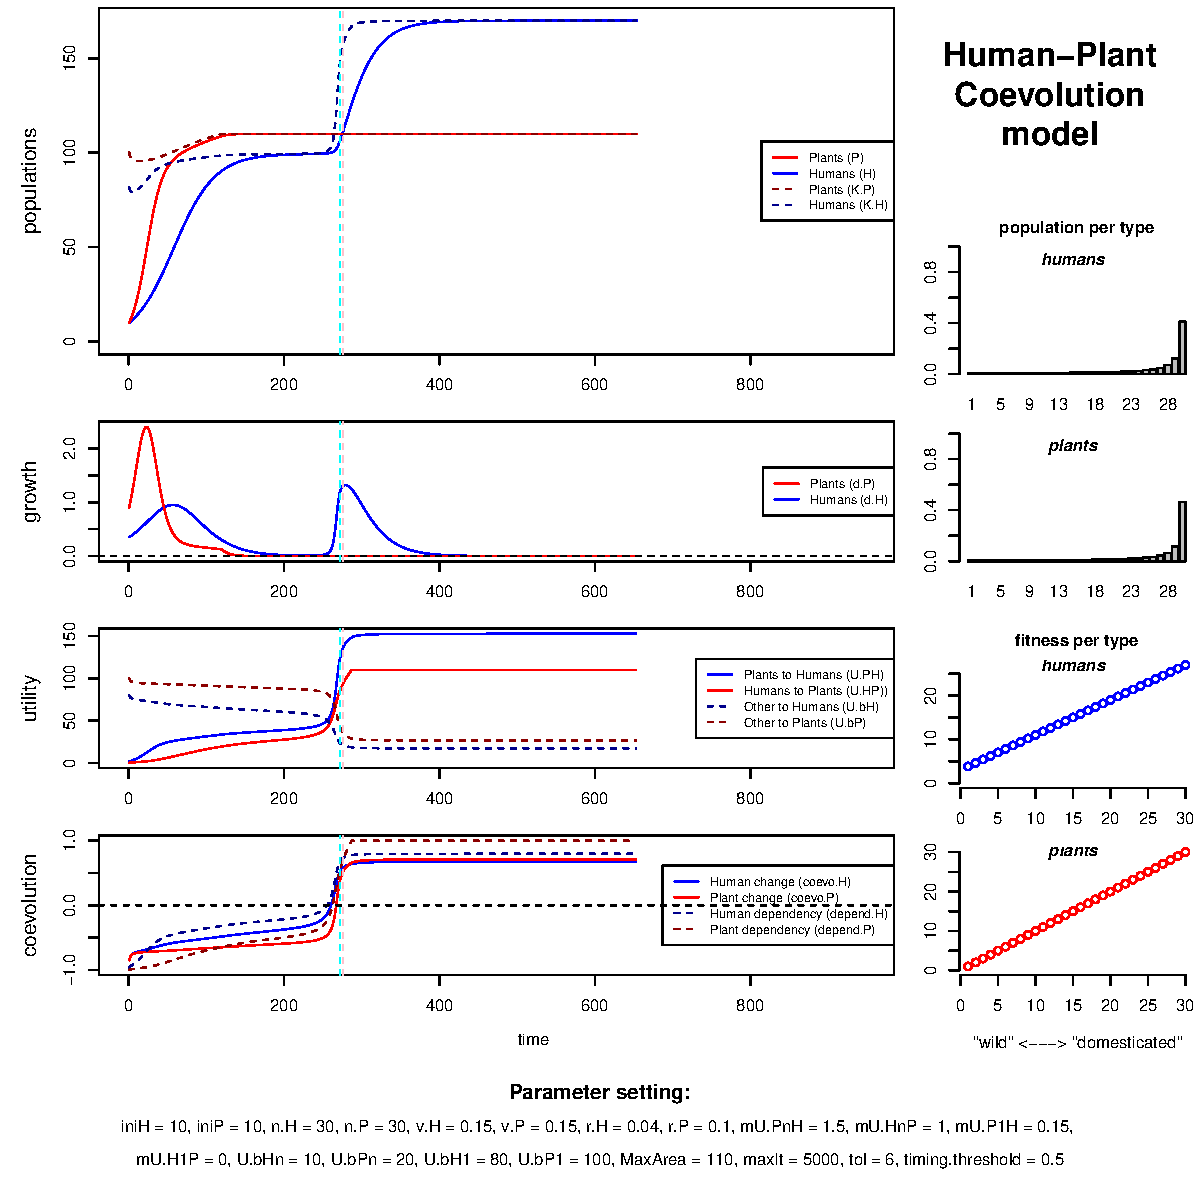
\includegraphics{hpcModel-exploration_files/figure-latex/1_run.coevo.bleep-plot-1.pdf}

\newpage

\hypertarget{coevolution-with-population-boom}{%
\section{Coevolution with population ``boom''}\label{coevolution-with-population-boom}}

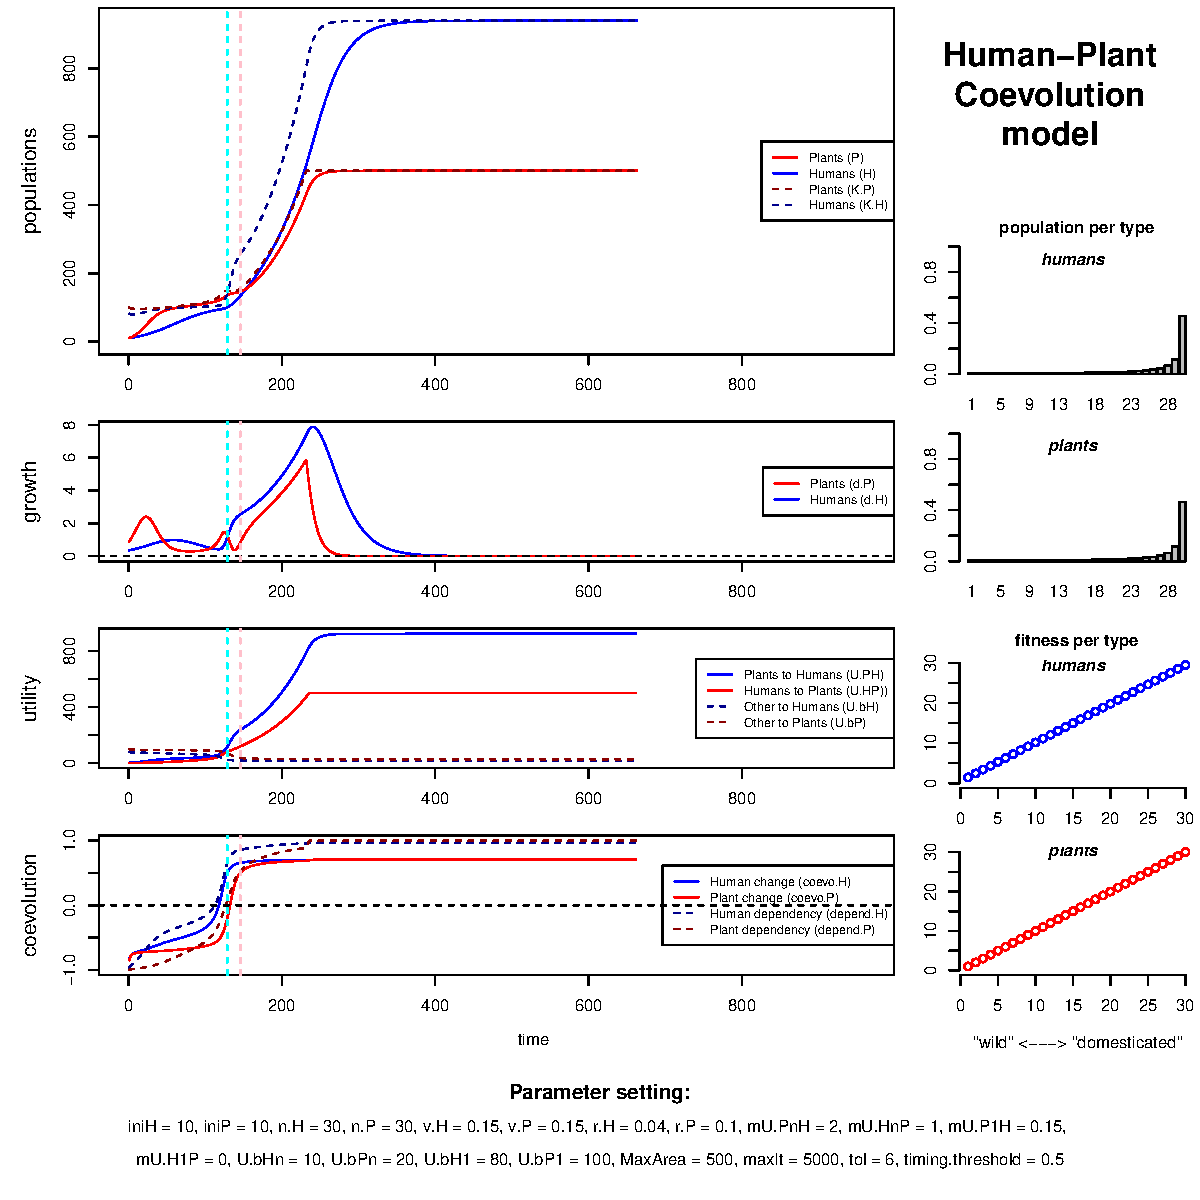
\includegraphics{hpcModel-exploration_files/figure-latex/1_run.coevo.boom-plot-1.pdf}

\newpage

\hypertarget{coevolution-with-long-population-boom}{%
\section{Coevolution with long population ``boom''}\label{coevolution-with-long-population-boom}}

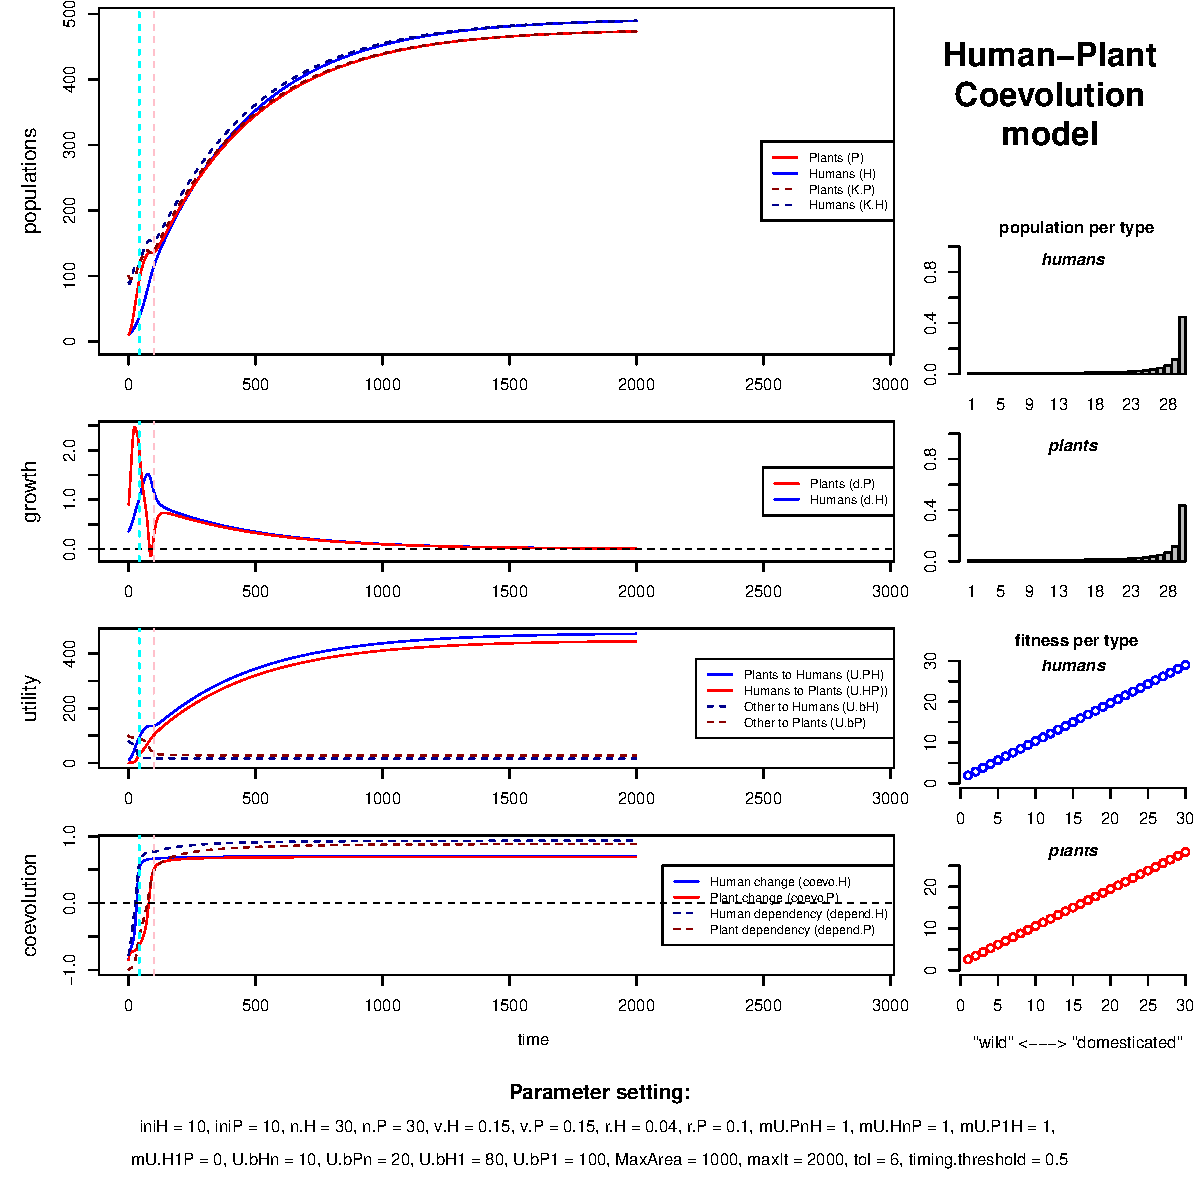
\includegraphics{hpcModel-exploration_files/figure-latex/1_run.coevo.long.boom-plot-1.pdf}

\newpage

\hypertarget{semi-coevolution-stationary-point}{%
\section{Semi-coevolution (stationary point)}\label{semi-coevolution-stationary-point}}

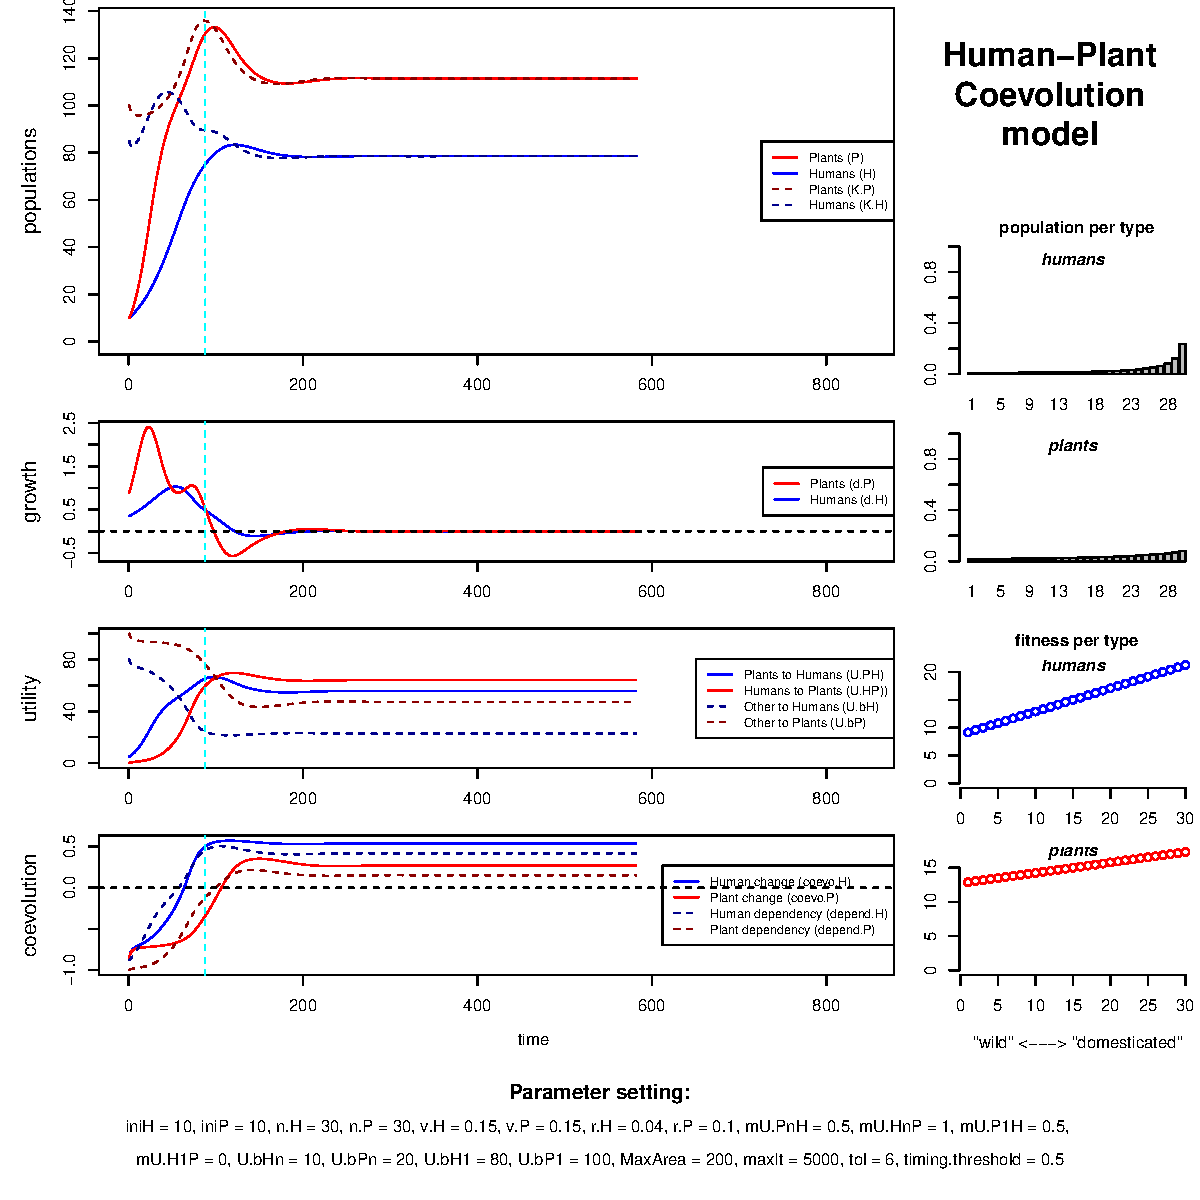
\includegraphics{hpcModel-exploration_files/figure-latex/1_run.semicoevo-plot-1.pdf}

\newpage

\hypertarget{semi-coevolution-oscillations}{%
\section{Semi-coevolution (oscillations)}\label{semi-coevolution-oscillations}}

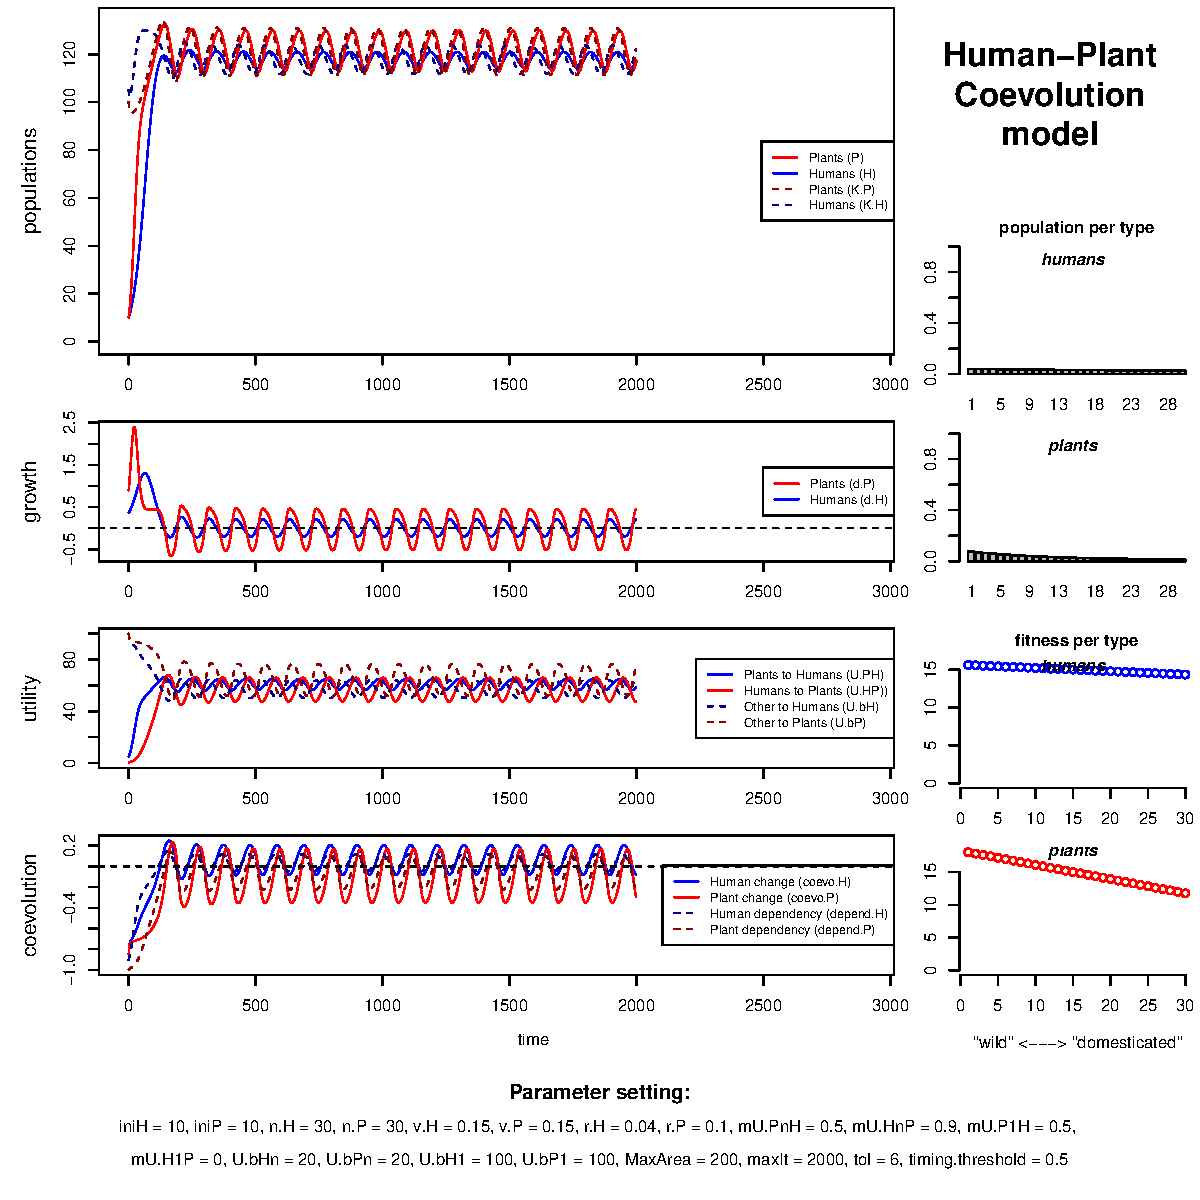
\includegraphics{hpcModel-exploration_files/figure-latex/1_run.semicoevo.osc1-plot-1.pdf}

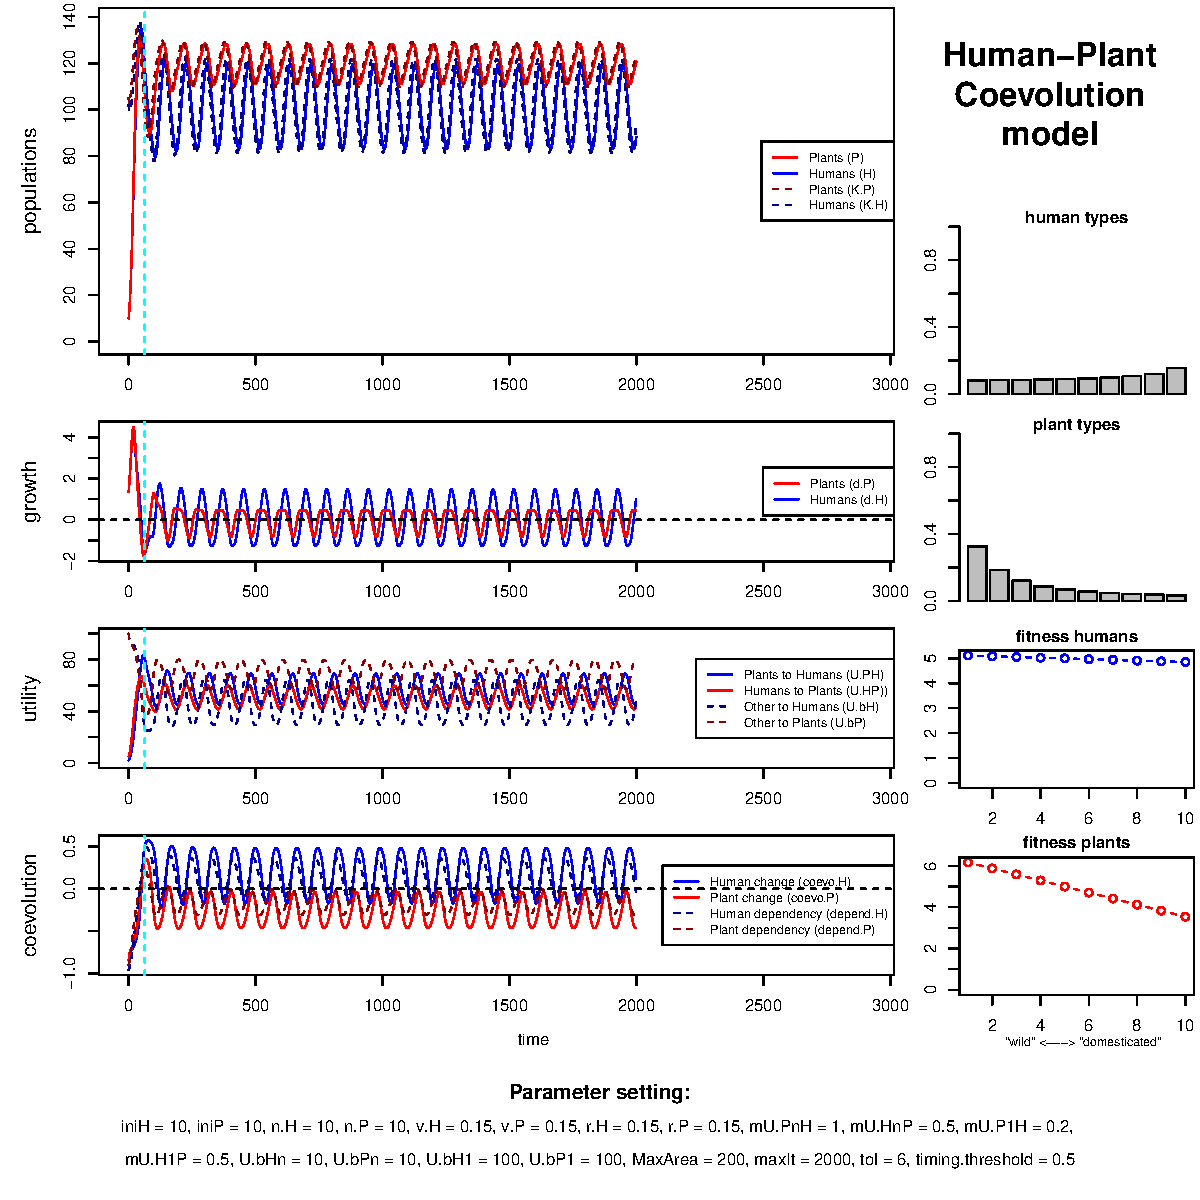
\includegraphics{hpcModel-exploration_files/figure-latex/1_run.semicoevo.osc2-plot-1.pdf}

\hypertarget{one-parameter-exploration}{%
\chapter{One parameter exploration}\label{one-parameter-exploration}}

\newpage

\hypertarget{full-example-tableplot-alternatives}{%
\section{Full example (table+plot alternatives)}\label{full-example-tableplot-alternatives}}

\hypertarget{utility-per-capita-of-type-n-plants-to-humans-baru_p_nh}{%
\subsection{\texorpdfstring{utility per capita \textbf{of} type n plants \textbf{to} humans (\(\bar{U}_{P_{n}H}\)):}{utility per capita of type n plants to humans (\textbackslash bar\{U\}\_\{P\_\{n\}H\}):}}\label{utility-per-capita-of-type-n-plants-to-humans-baru_p_nh}}

\begin{table}[!h]

\caption{\label{tab:2mUPnHtablepdf}Parameter setting}
\centering
\begin{tabular}[t]{l|l}
\hline
parameter & value\\
\hline
iniH & 10\\
\hline
iniP & 10\\
\hline
n.H & 30\\
\hline
n.P & 30\\
\hline
v.H & 0.15\\
\hline
v.P & 0.15\\
\hline
r.H & 0.04\\
\hline
r.P & 0.1\\
\hline
mU.PnH & 0.5 - 2.5 (sample = 100 )\\
\hline
mU.HnP & 1\\
\hline
mU.P1H & 0.15\\
\hline
mU.H1P & 0\\
\hline
U.bHn & 10\\
\hline
U.bPn & 20\\
\hline
U.bH1 & 80\\
\hline
U.bP1 & 100\\
\hline
MaxArea & 200\\
\hline
\end{tabular}
\end{table}

\begin{figure}
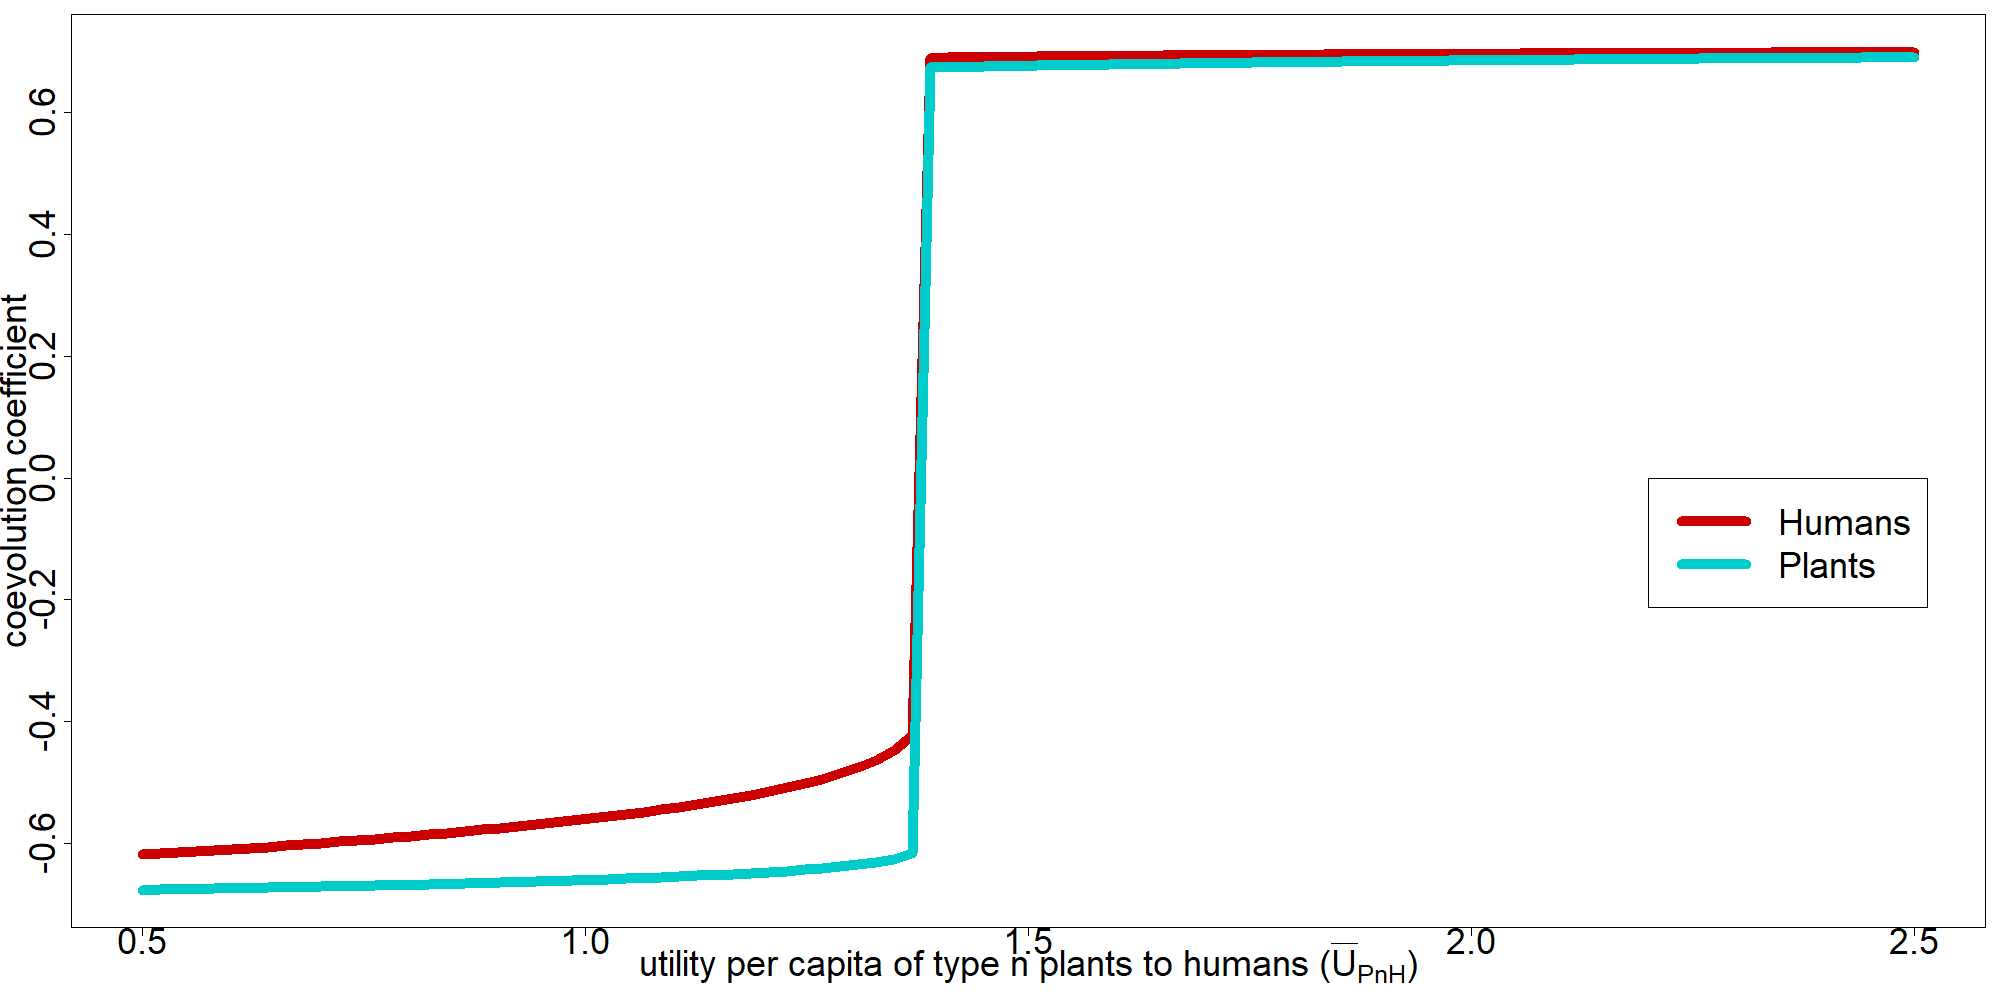
\includegraphics[width=1\linewidth]{plots/2_onePar-mU.PnH_ggbifplot} \caption{Bifurcation plot (ggplot2)}\label{fig:2mUPnHbifplot1print}
\end{figure}

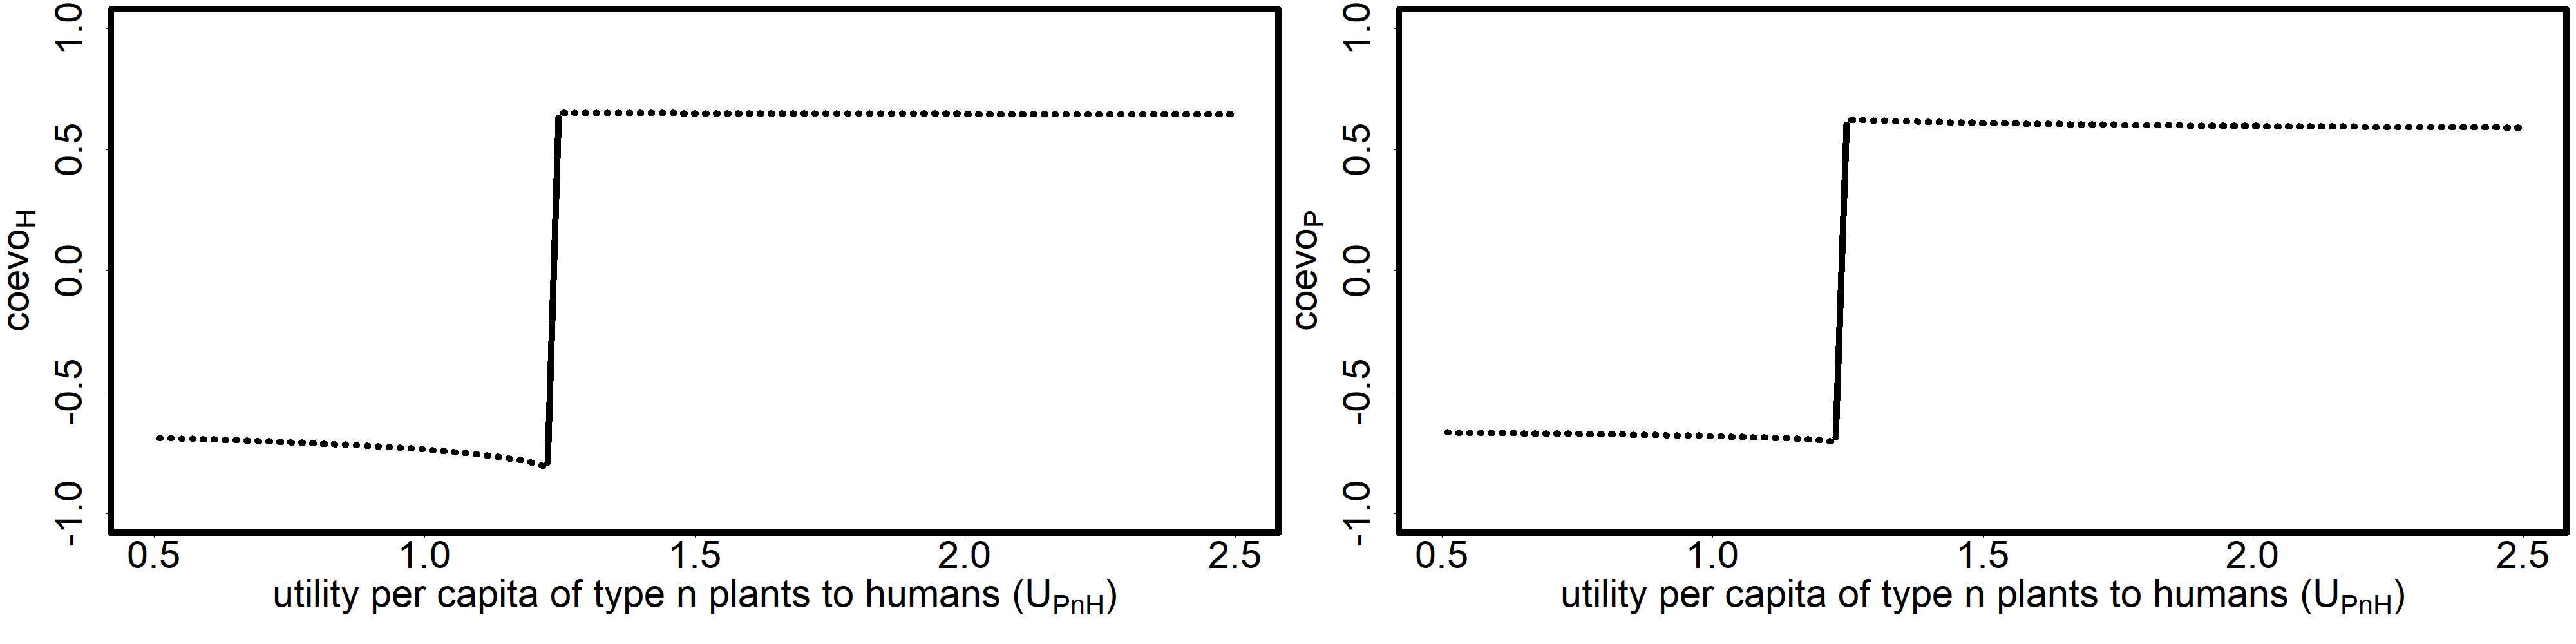
\includegraphics[width=1\linewidth]{plots/2_onePar-mU.PnH_bifplot-pair}

\newpage

\hypertarget{exploration-on-default-setting-for-each-parameter}{%
\section{Exploration on `default' setting for each parameter:}\label{exploration-on-default-setting-for-each-parameter}}

\hypertarget{initial-populations-of-humans-and-plants-init_hinit_p}{%
\subsection{\texorpdfstring{Initial populations of humans and plants (\(init_{H},\,init_{P}\))}{Initial populations of humans and plants (init\_\{H\},\textbackslash,init\_\{P\})}}\label{initial-populations-of-humans-and-plants-init_hinit_p}}

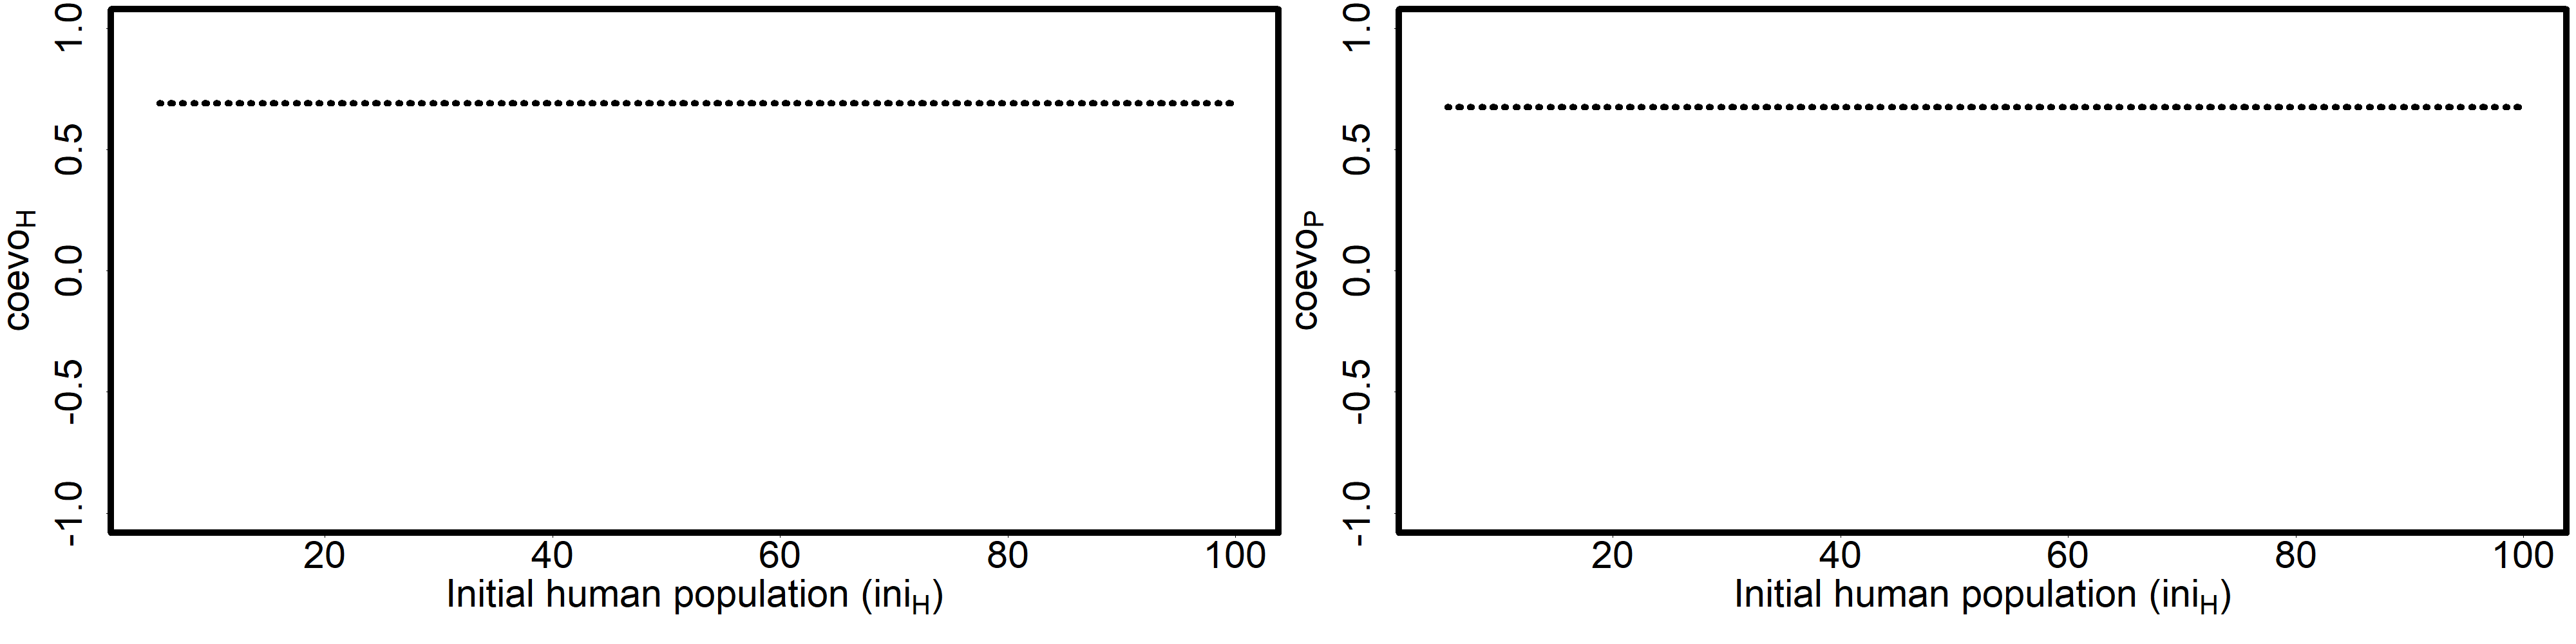
\includegraphics[width=1\linewidth]{plots/2_onePar-init.H_bifplot-pair}

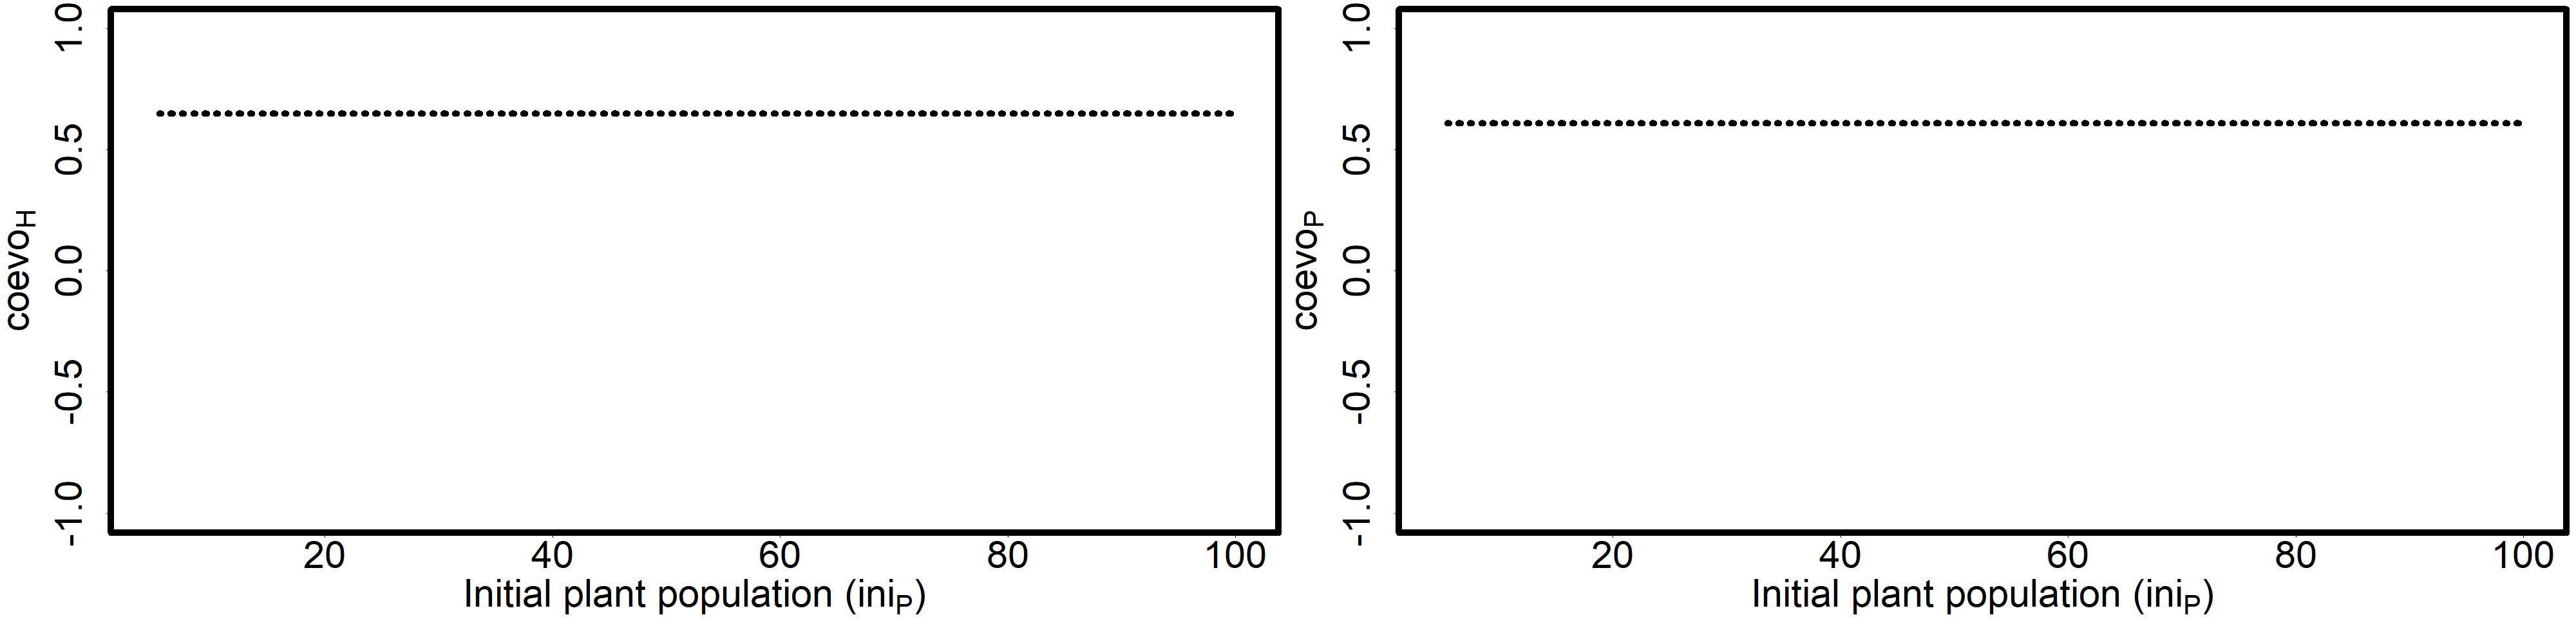
\includegraphics[width=1\linewidth]{plots/2_onePar-init.P_bifplot-pair}

\hypertarget{number-of-types-of-humans-and-plants-n_hn_p}{%
\subsection{\texorpdfstring{Number of types of humans and plants (\(n_{H},\,n_{P}\)):}{Number of types of humans and plants (n\_\{H\},\textbackslash,n\_\{P\}):}}\label{number-of-types-of-humans-and-plants-n_hn_p}}

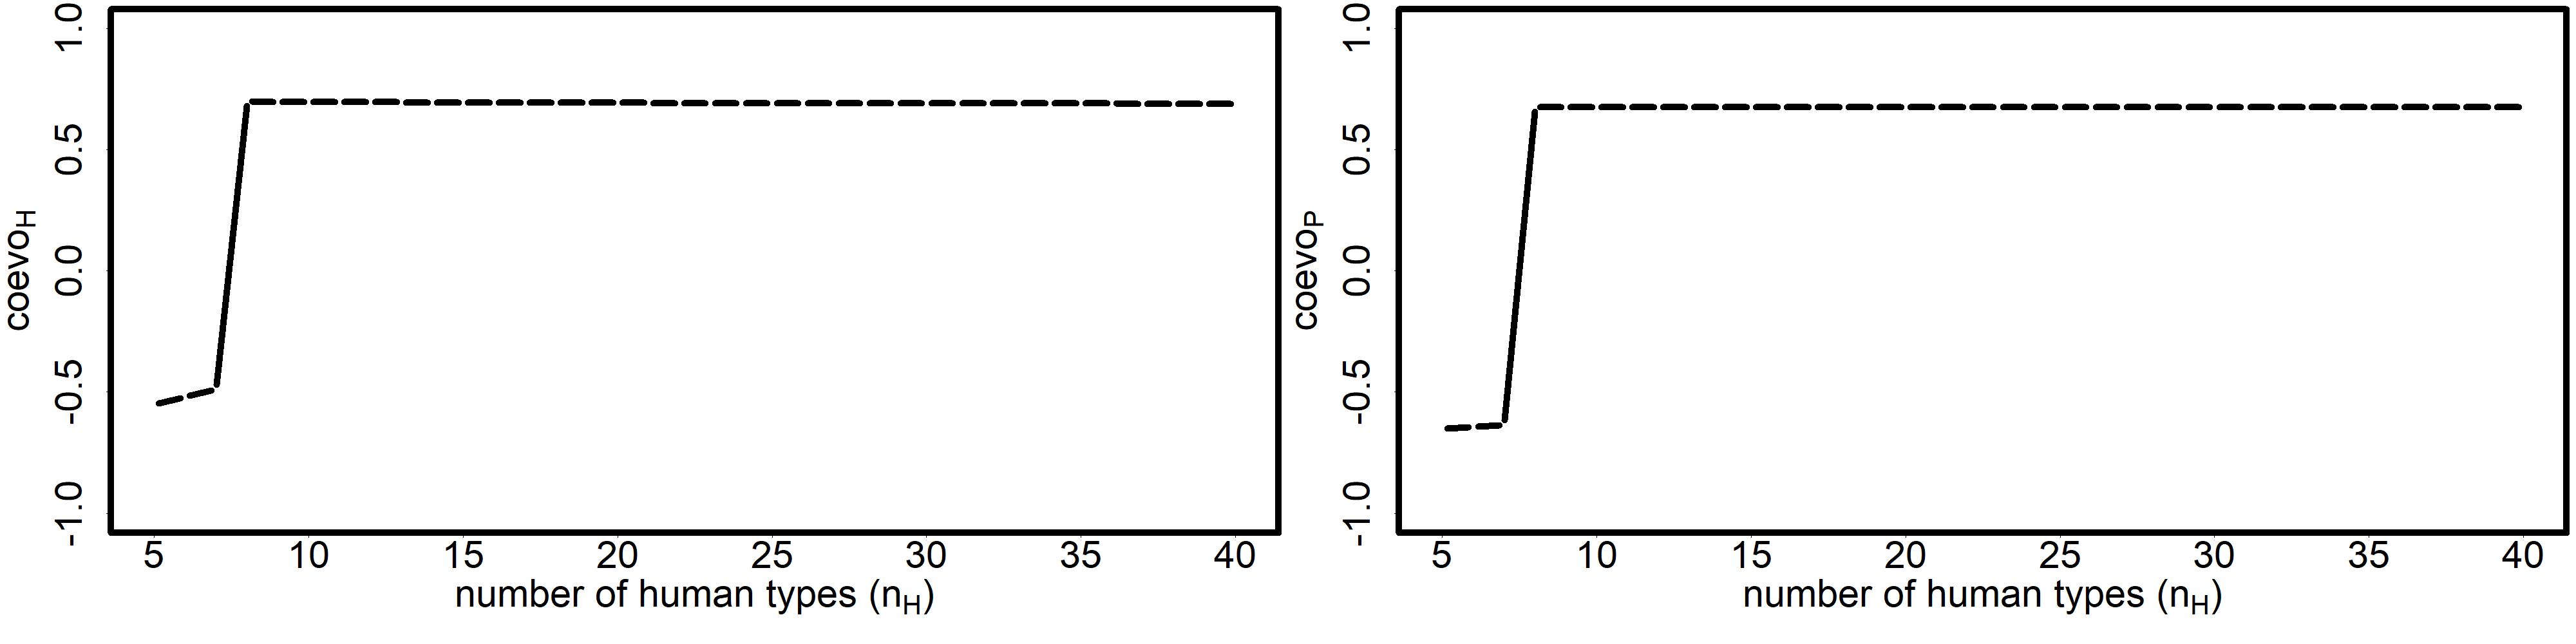
\includegraphics[width=1\linewidth]{plots/2_onePar-n.H_bifplot-pair}

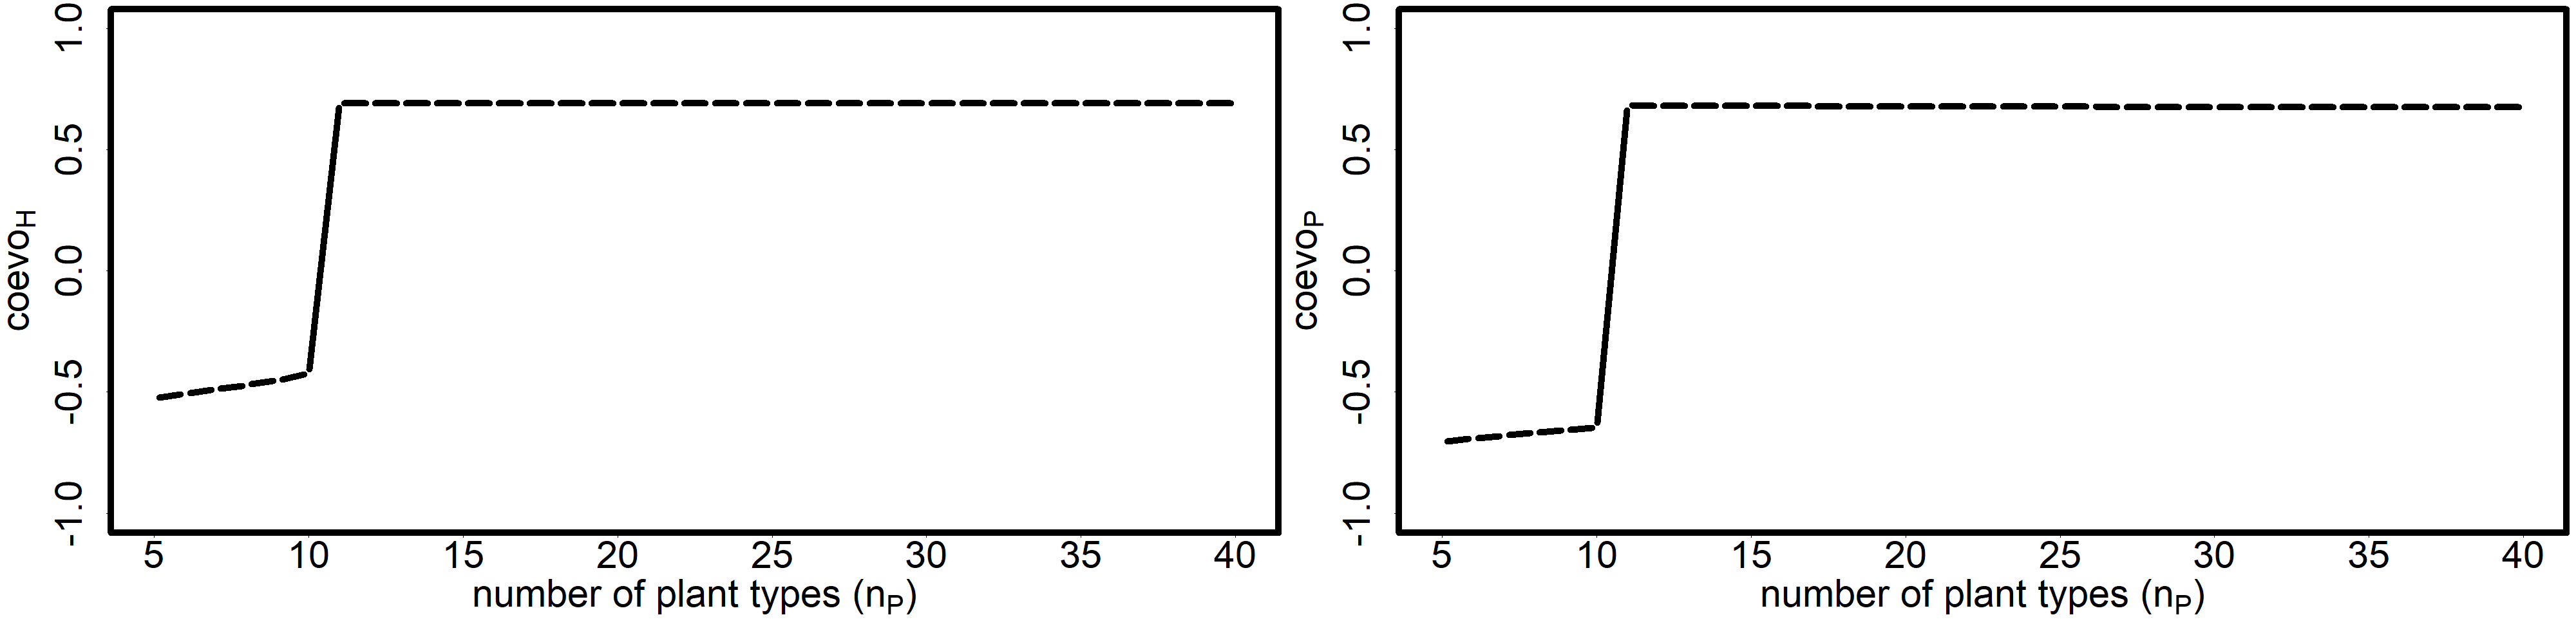
\includegraphics[width=1\linewidth]{plots/2_onePar-n.P_bifplot-pair}

\hypertarget{level-of-undirected-variation-in-humans-and-plants-v_hv_p}{%
\subsection{\texorpdfstring{level of undirected variation in humans and plants (\(v_{H},\,v_{P}\)):}{level of undirected variation in humans and plants (v\_\{H\},\textbackslash,v\_\{P\}):}}\label{level-of-undirected-variation-in-humans-and-plants-v_hv_p}}

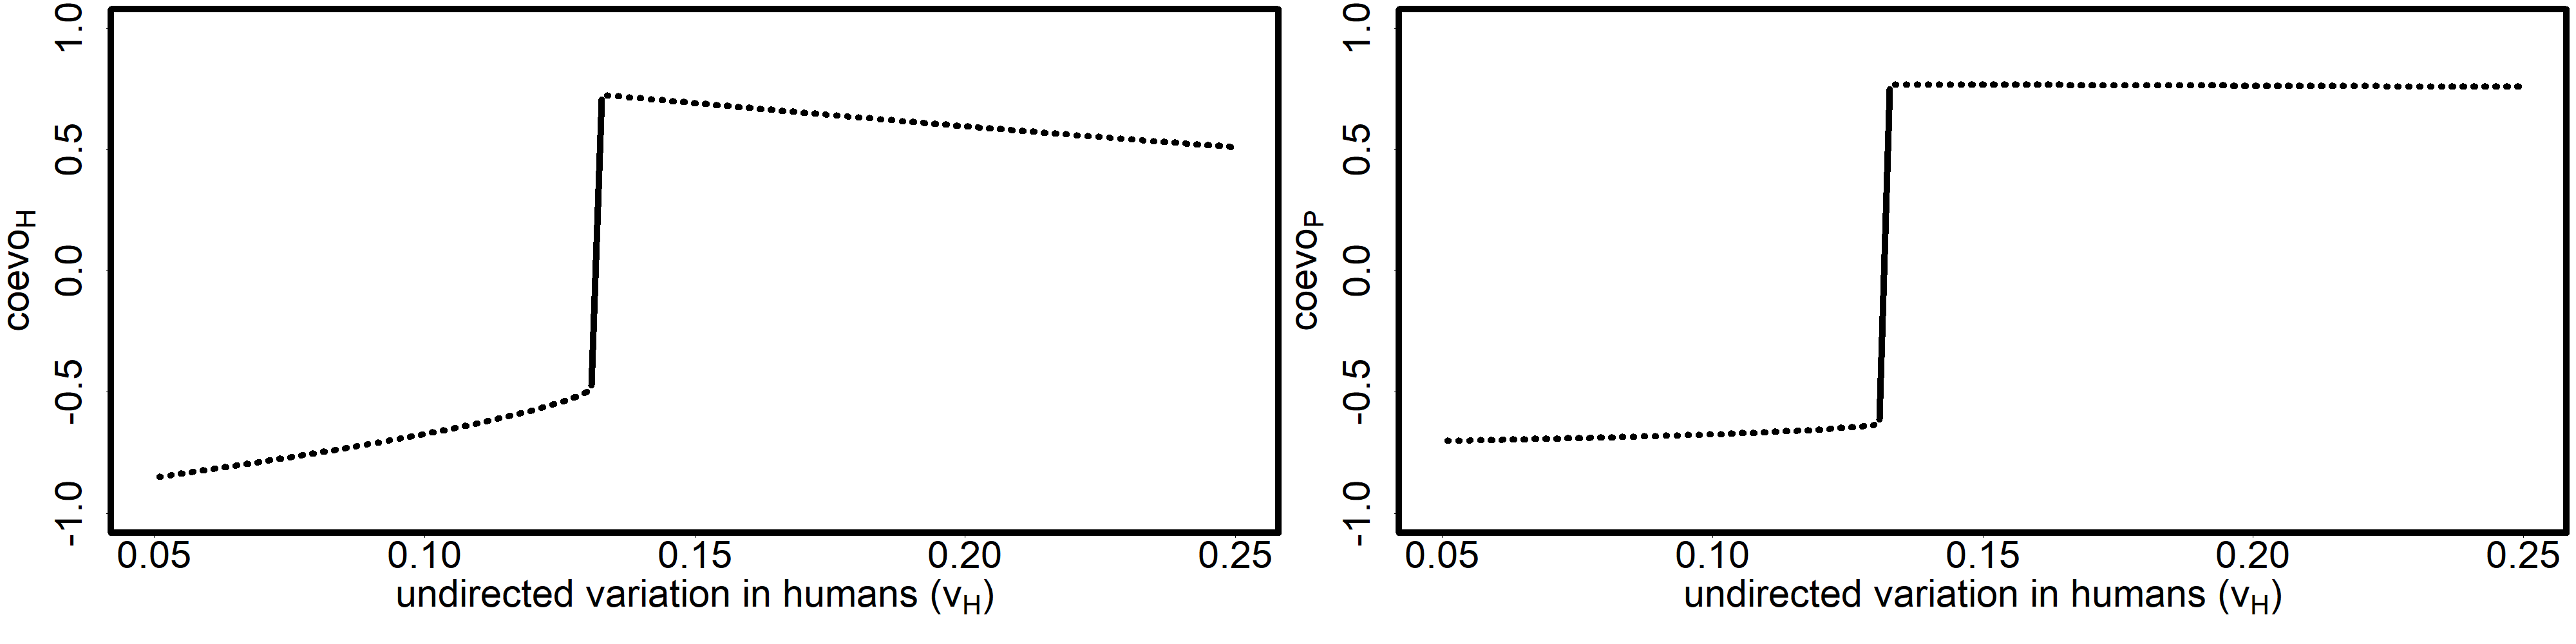
\includegraphics[width=1\linewidth]{plots/2_onePar-v.H_bifplot-pair}

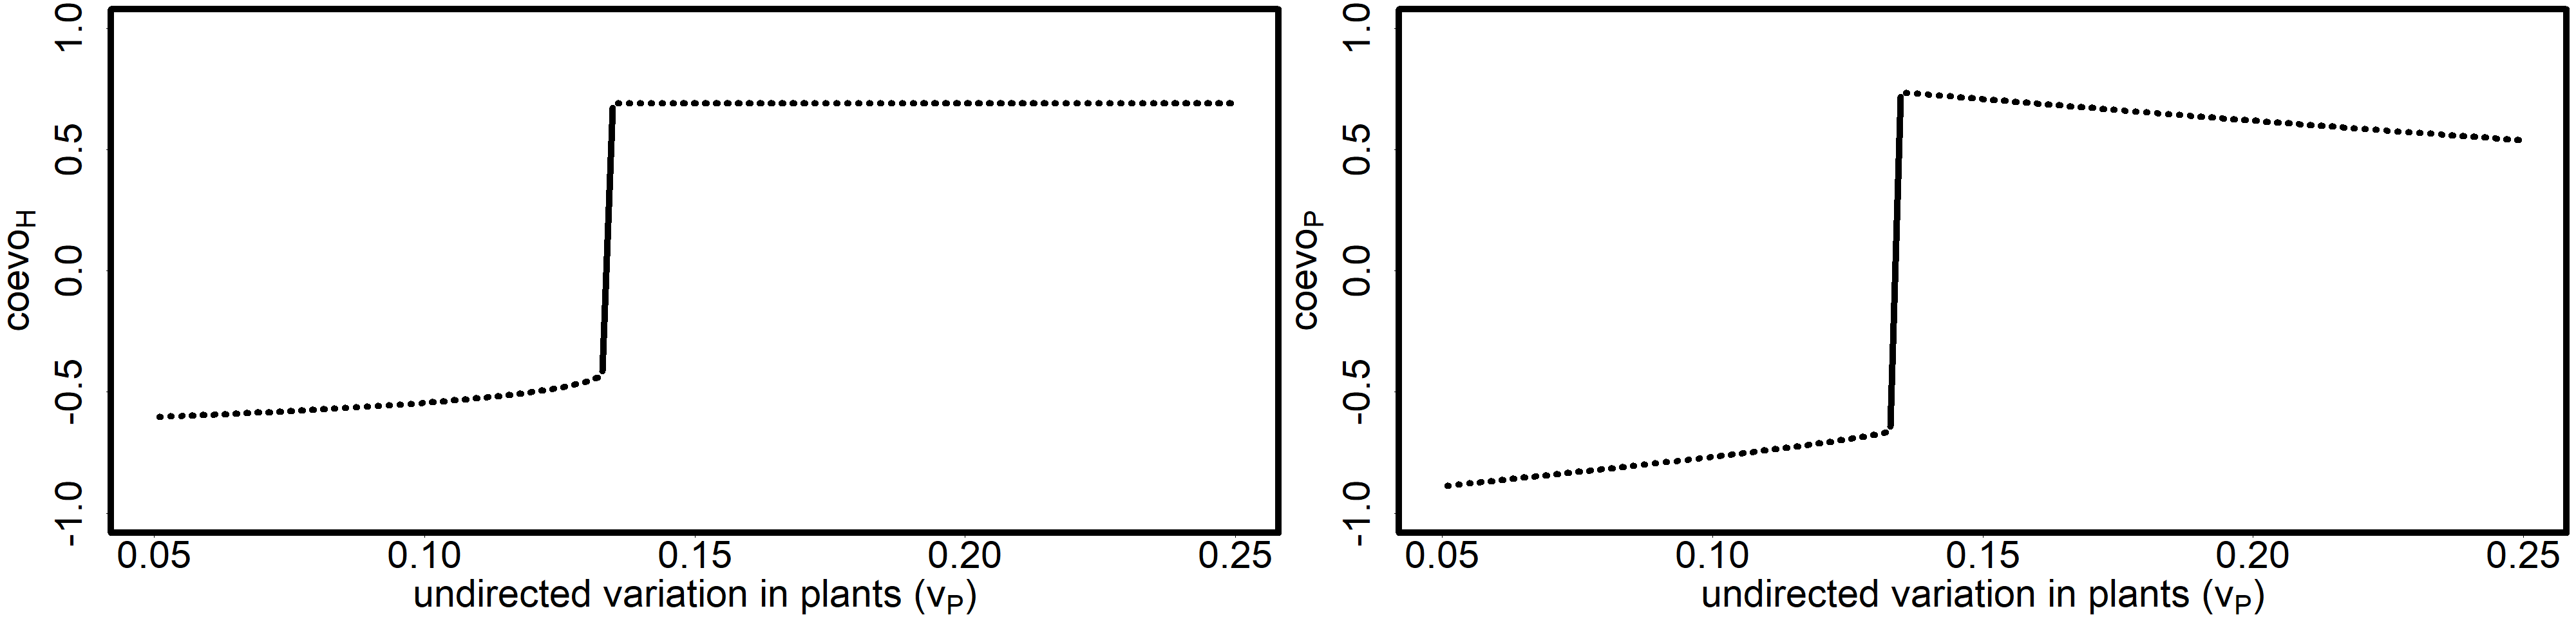
\includegraphics[width=1\linewidth]{plots/2_onePar-v.P_bifplot-pair}

\hypertarget{intrinsic-growth-rates-for-human-and-plant-populations-r_hr_p}{%
\subsection{\texorpdfstring{intrinsic growth rates for human and plant populations (\(r_{H},\,r_{P}\)):}{intrinsic growth rates for human and plant populations (r\_\{H\},\textbackslash,r\_\{P\}):}}\label{intrinsic-growth-rates-for-human-and-plant-populations-r_hr_p}}

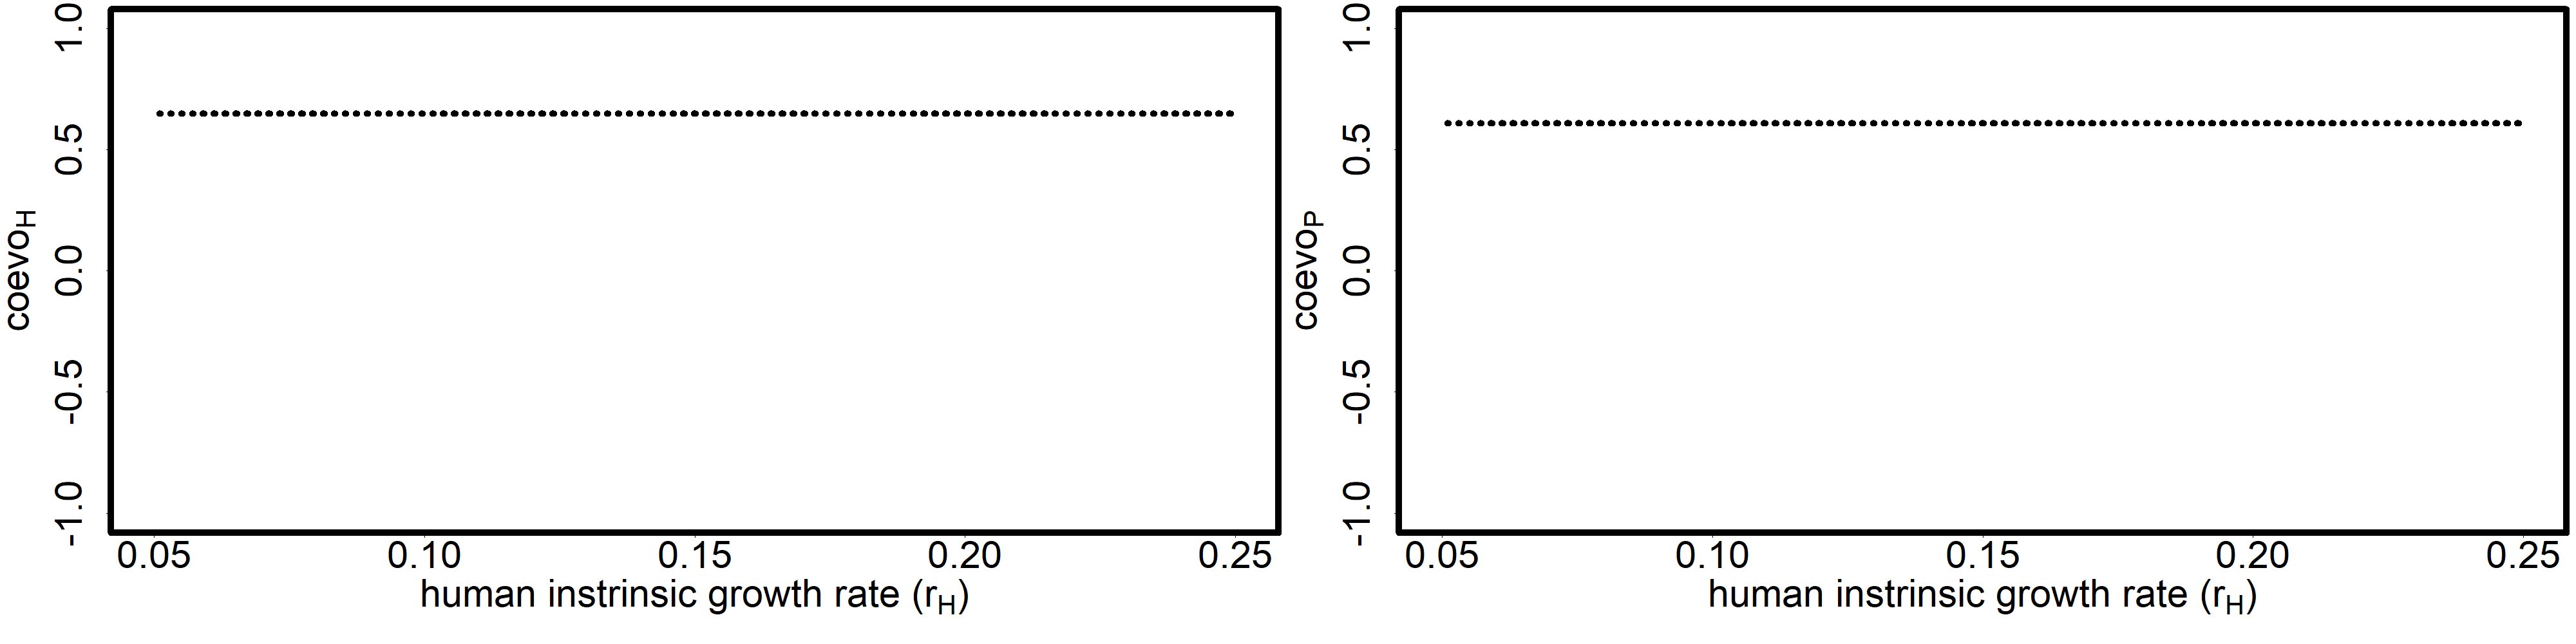
\includegraphics[width=1\linewidth]{plots/2_onePar-r.H_bifplot-pair}

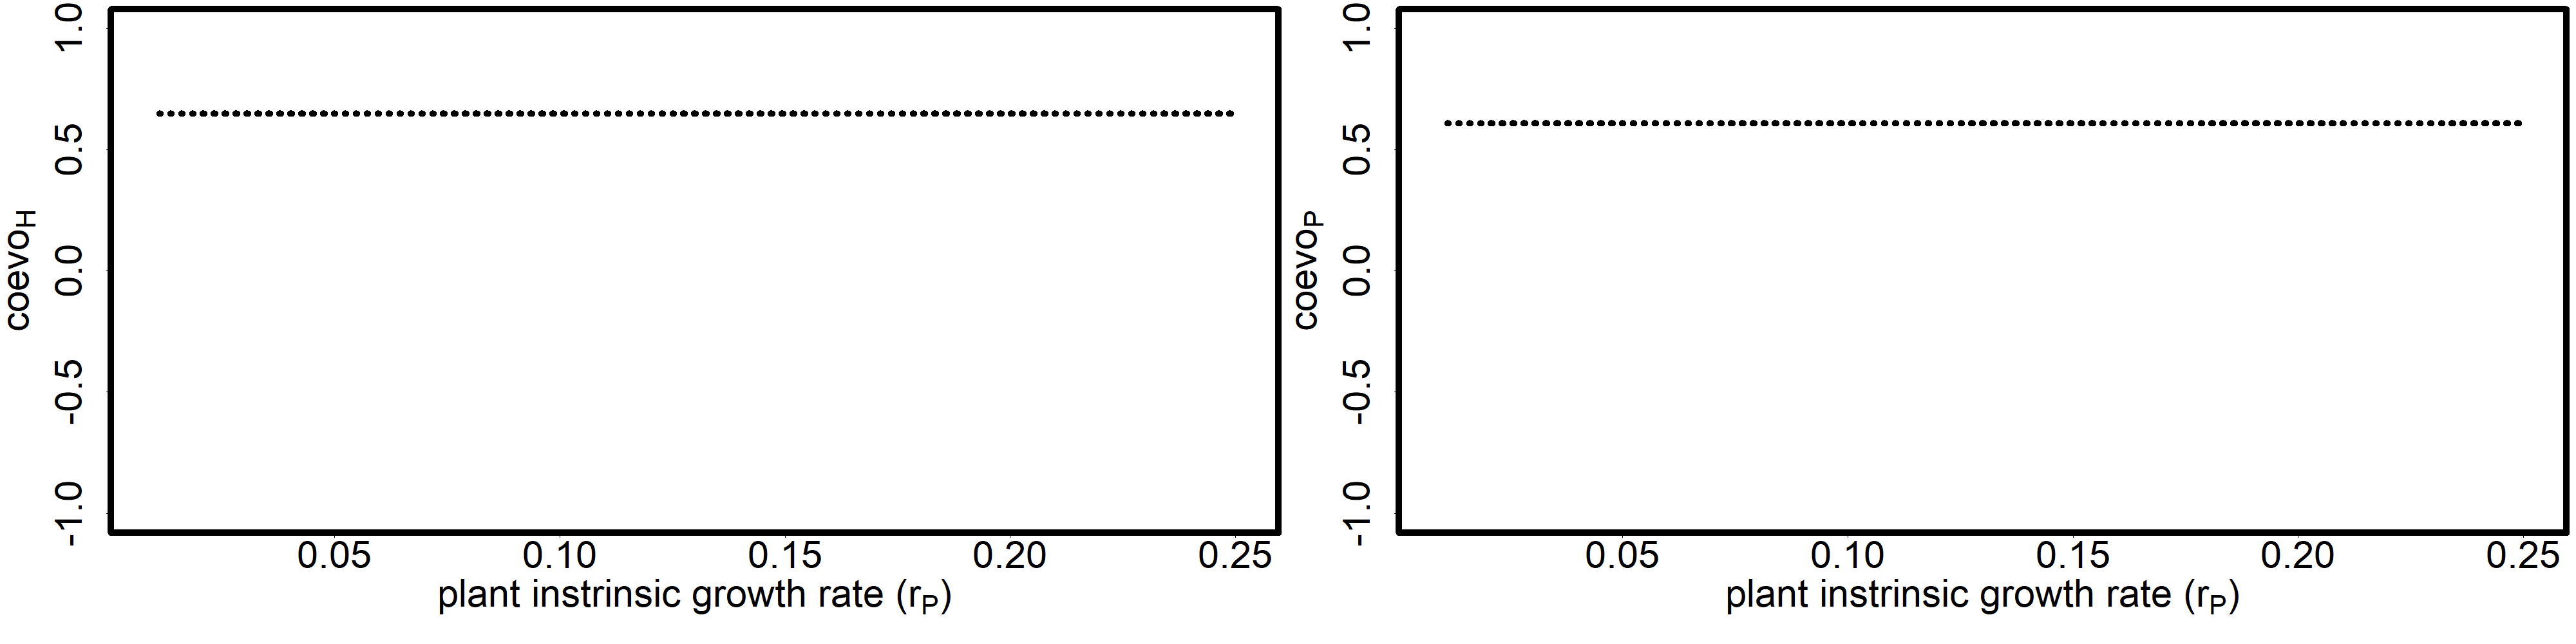
\includegraphics[width=1\linewidth]{plots/2_onePar-r.P_bifplot-pair}

\hypertarget{utility-per-capita-of-type-n-plants-to-humans-baru_p_nh-1}{%
\subsection{\texorpdfstring{utility per capita \textbf{of} type n plants \textbf{to} humans (\(\bar{U}_{P_{n}H}\)):}{utility per capita of type n plants to humans (\textbackslash bar\{U\}\_\{P\_\{n\}H\}):}}\label{utility-per-capita-of-type-n-plants-to-humans-baru_p_nh-1}}

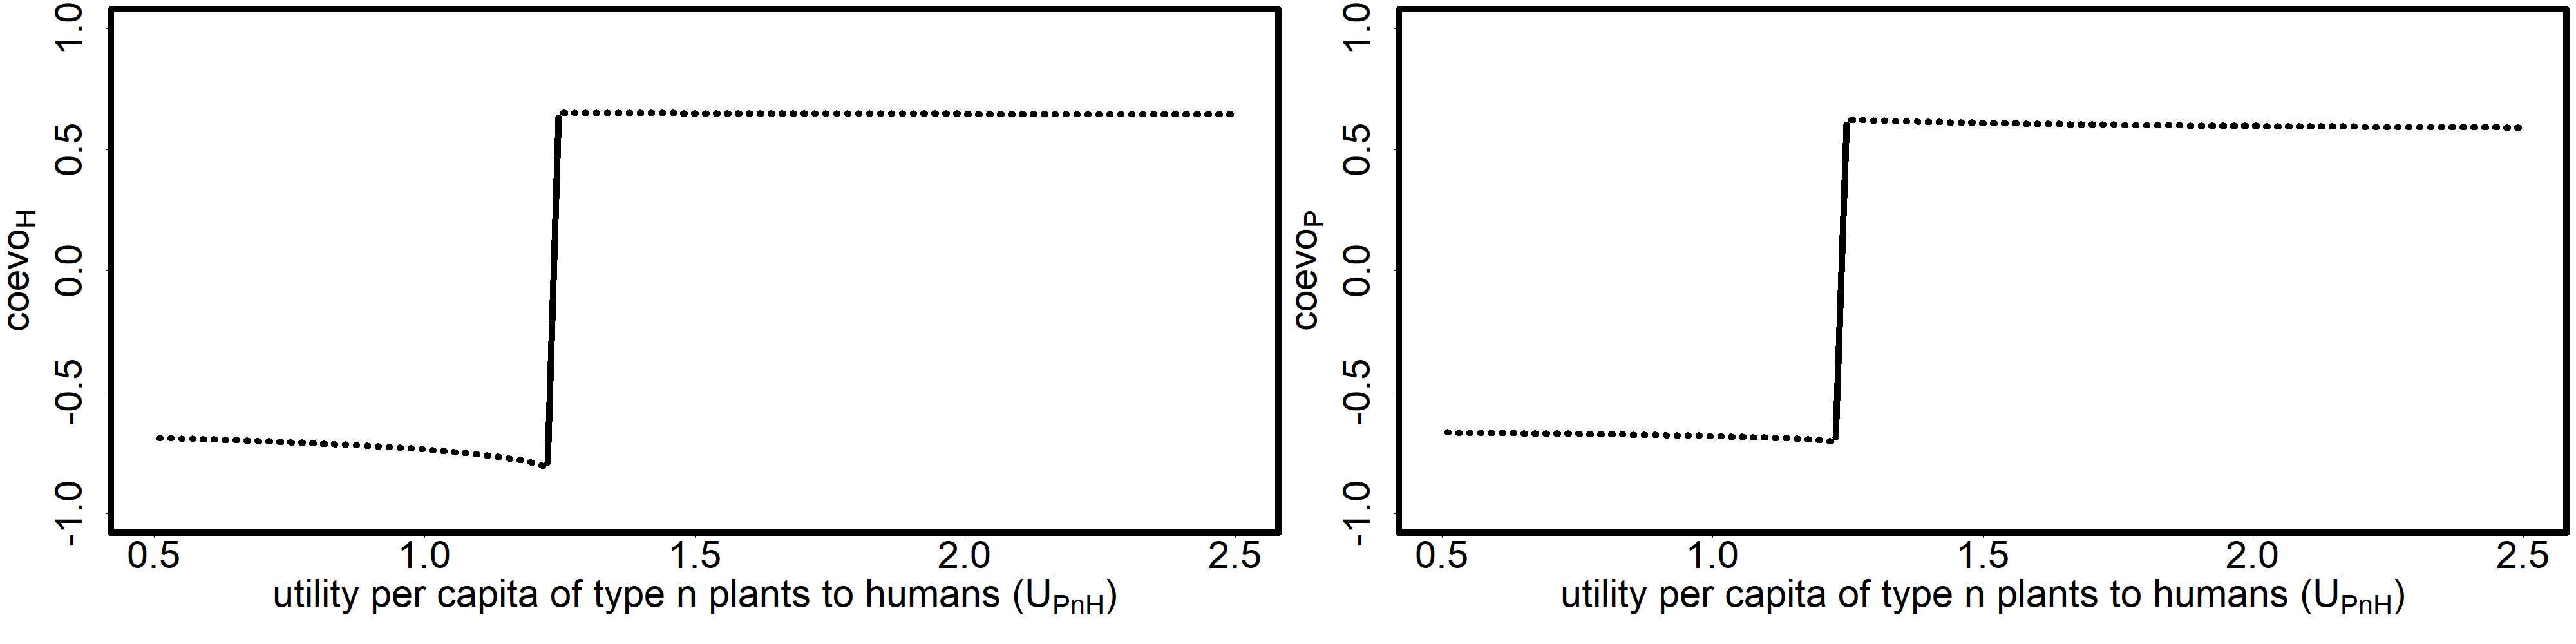
\includegraphics[width=1\linewidth]{plots/2_onePar-mU.PnH_bifplot-pair}

\hypertarget{utility-per-capita-of-type-n-human-to-plants-baru_h_np}{%
\subsection{\texorpdfstring{utility per capita \textbf{of} type n human \textbf{to} plants (\(\bar{U}_{H_{n}P}\)):}{utility per capita of type n human to plants (\textbackslash bar\{U\}\_\{H\_\{n\}P\}):}}\label{utility-per-capita-of-type-n-human-to-plants-baru_h_np}}

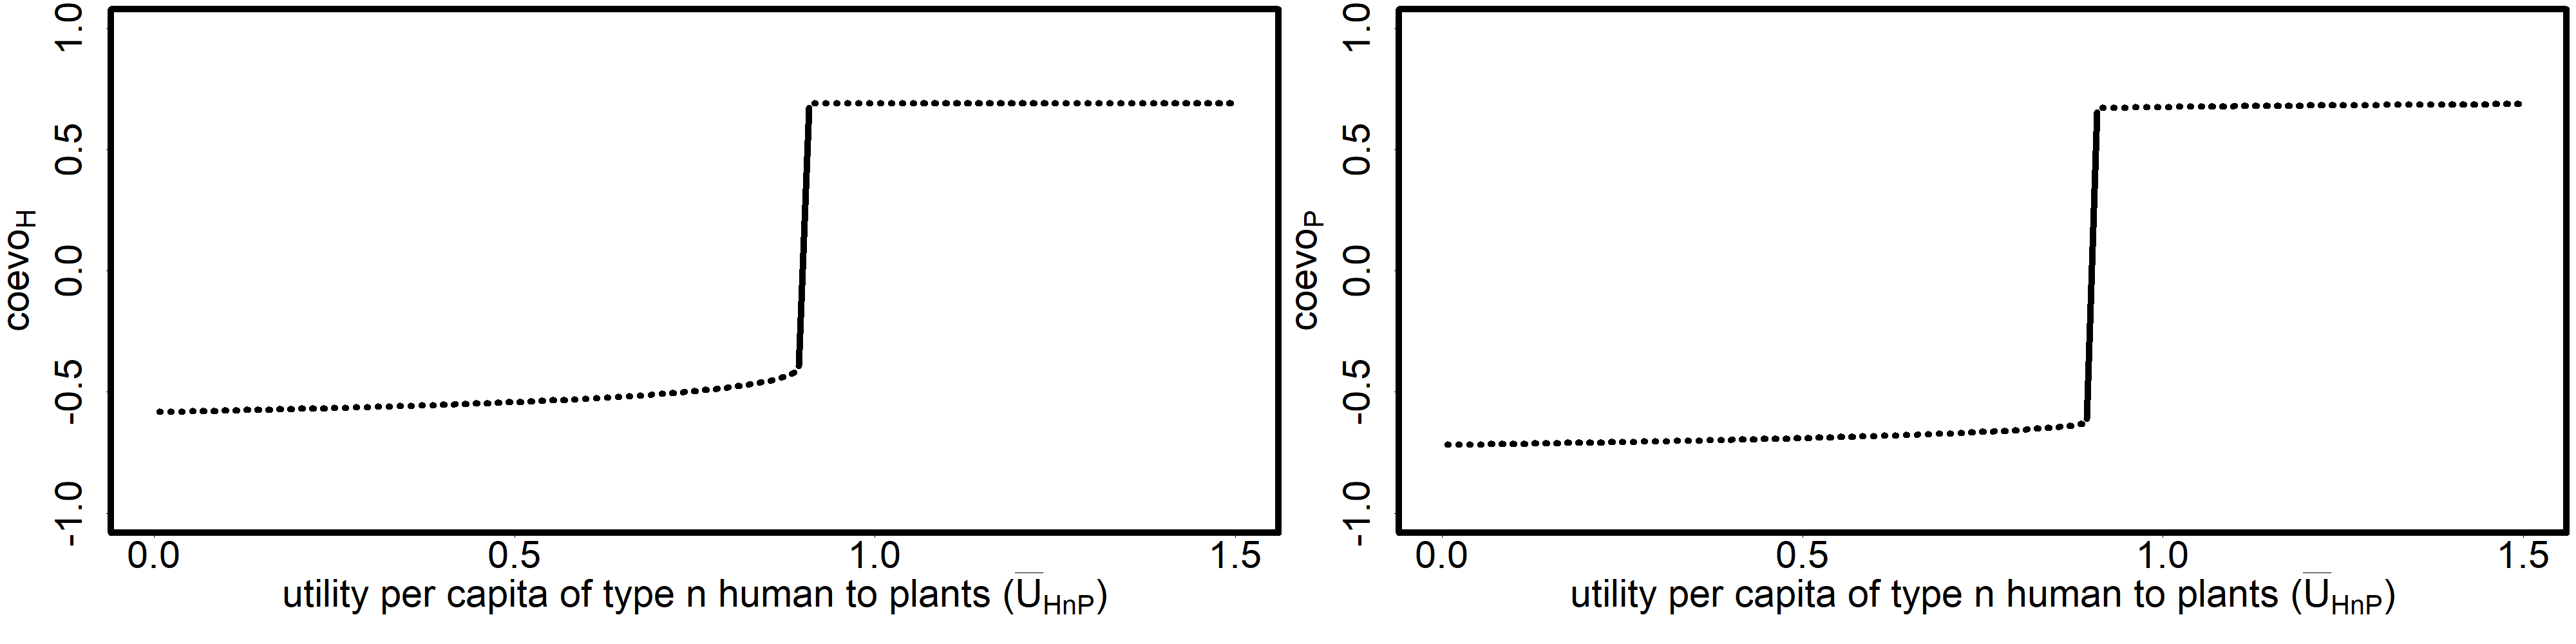
\includegraphics[width=1\linewidth]{plots/2_onePar-mU.HnP_bifplot-pair}

\hypertarget{utility-per-capita-of-type-1-plants-to-humans-baru_p_1h}{%
\subsection{\texorpdfstring{utility per capita \textbf{of} type 1 plants \textbf{to} humans (\(\bar{U}_{P_{1}H}\)):}{utility per capita of type 1 plants to humans (\textbackslash bar\{U\}\_\{P\_\{1\}H\}):}}\label{utility-per-capita-of-type-1-plants-to-humans-baru_p_1h}}

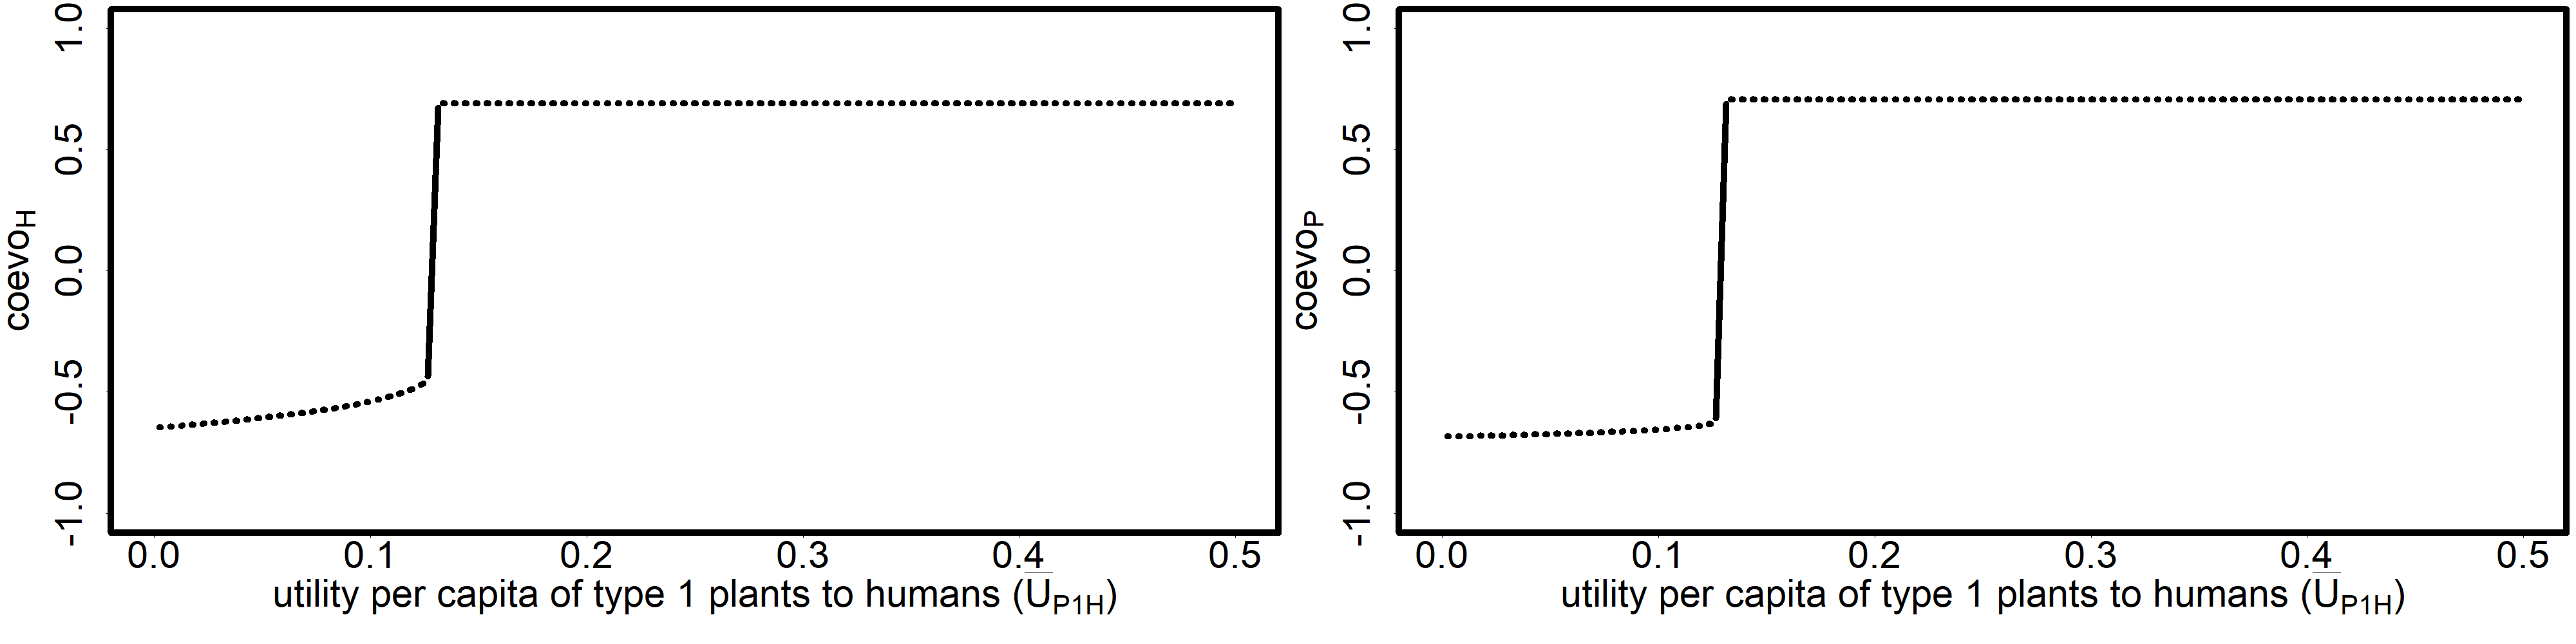
\includegraphics[width=1\linewidth]{plots/2_onePar-mU.P1H_bifplot-pair}

\hypertarget{utility-per-capita-of-type-1-humans-to-plants-baru_h_1p}{%
\subsection{\texorpdfstring{utility per capita \textbf{of} type 1 humans \textbf{to} plants (\(\bar{U}_{H_{1}P}\)):}{utility per capita of type 1 humans to plants (\textbackslash bar\{U\}\_\{H\_\{1\}P\}):}}\label{utility-per-capita-of-type-1-humans-to-plants-baru_h_1p}}

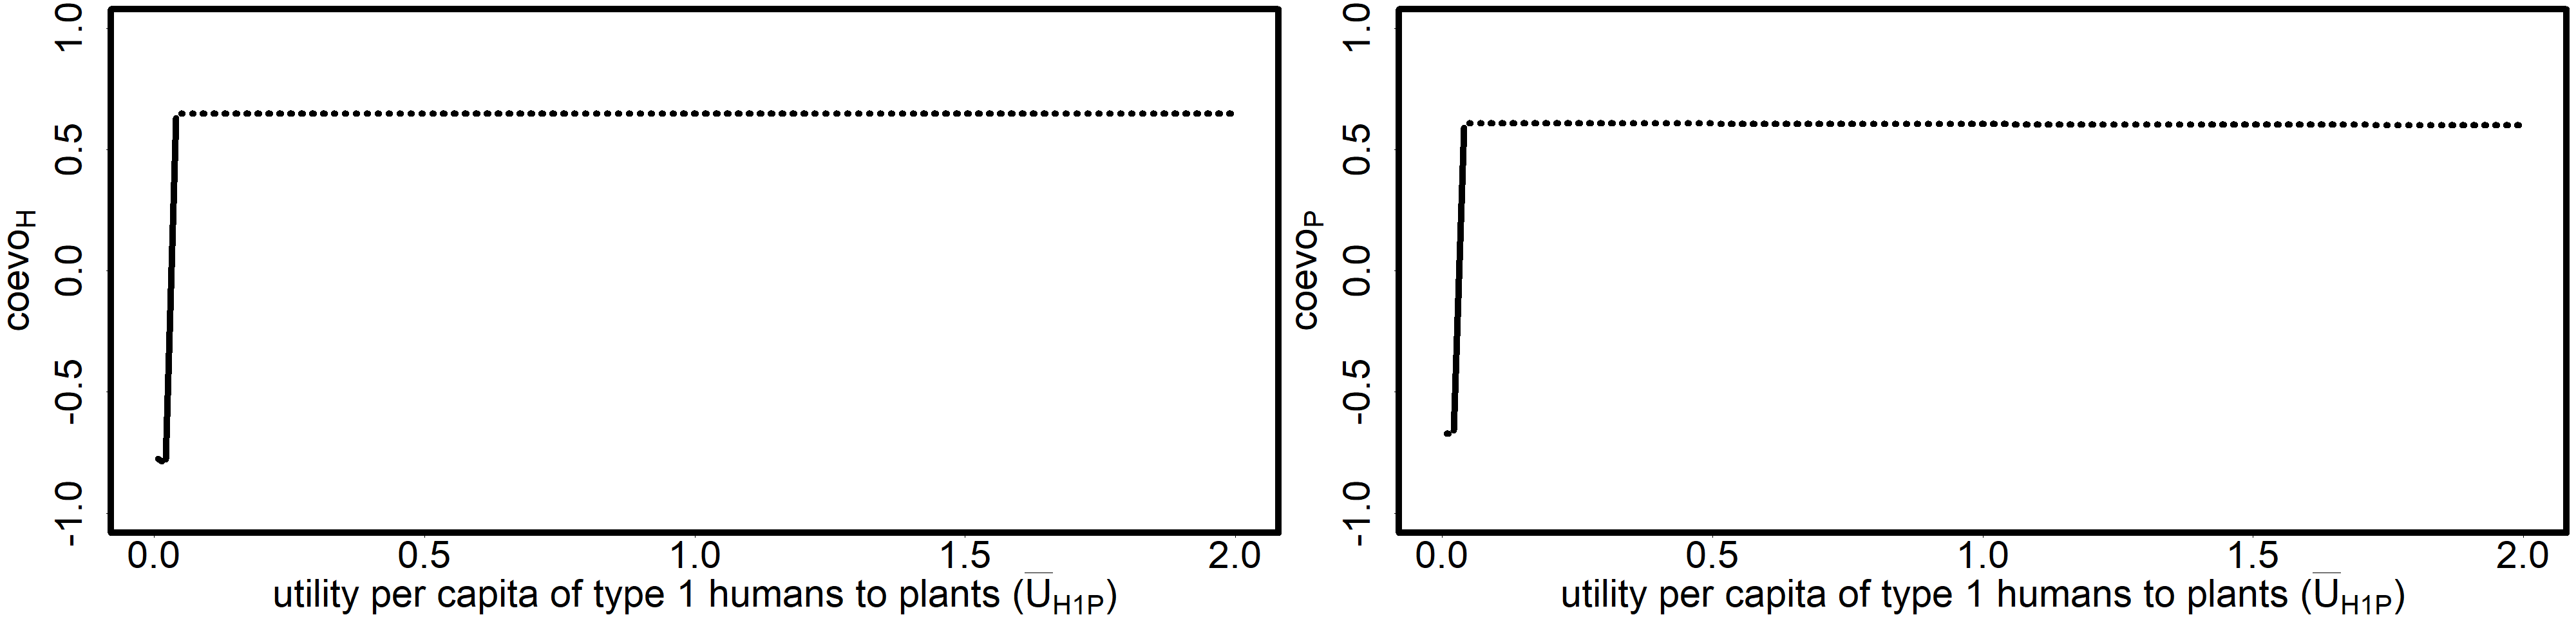
\includegraphics[width=1\linewidth]{plots/2_onePar-mU.H1P_bifplot-pair}

\hypertarget{utility-of-other-resources-to-humans-of-type-1-u_bh_1}{%
\subsection{\texorpdfstring{utility \textbf{of} other resources \textbf{to} humans of type 1 (\(U_{bH_{1}}\)):}{utility of other resources to humans of type 1 (U\_\{bH\_\{1\}\}):}}\label{utility-of-other-resources-to-humans-of-type-1-u_bh_1}}

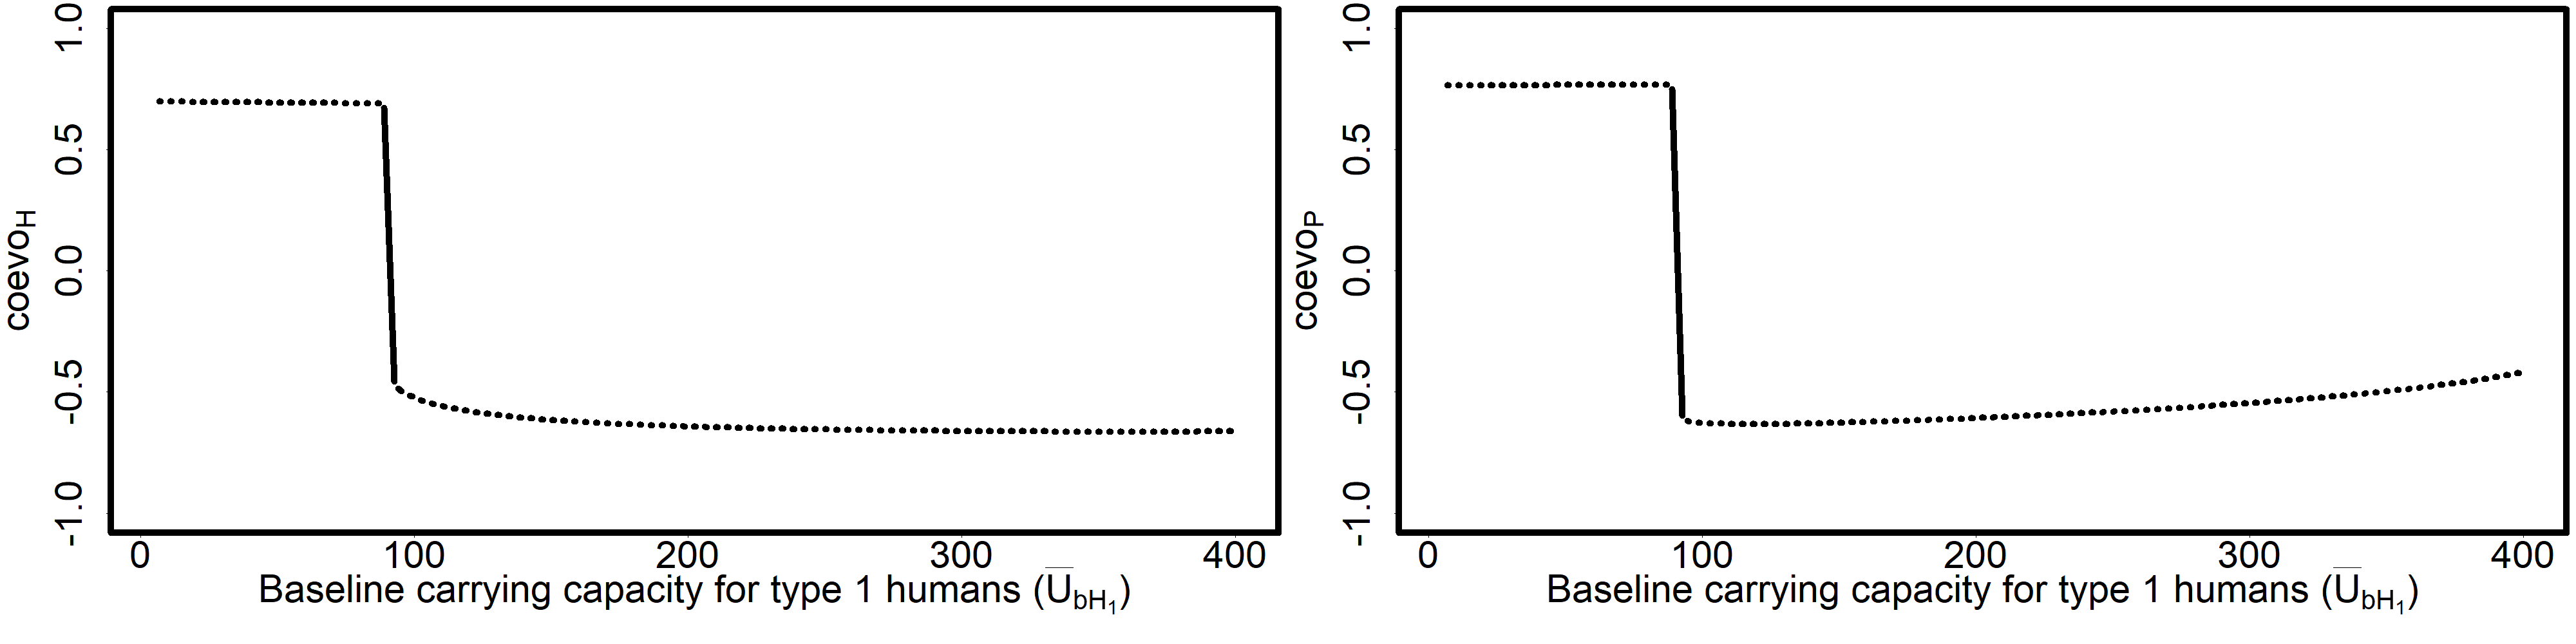
\includegraphics[width=1\linewidth]{plots/2_onePar-U.bH1_bifplot-pair}

\hypertarget{utility-of-non-anthropic-space-to-type-1-plants-u_bp_1}{%
\subsection{\texorpdfstring{utility \textbf{of} non-anthropic space \textbf{to} type 1 plants (\(U_{bP_{1}}\)):}{utility of non-anthropic space to type 1 plants (U\_\{bP\_\{1\}\}):}}\label{utility-of-non-anthropic-space-to-type-1-plants-u_bp_1}}

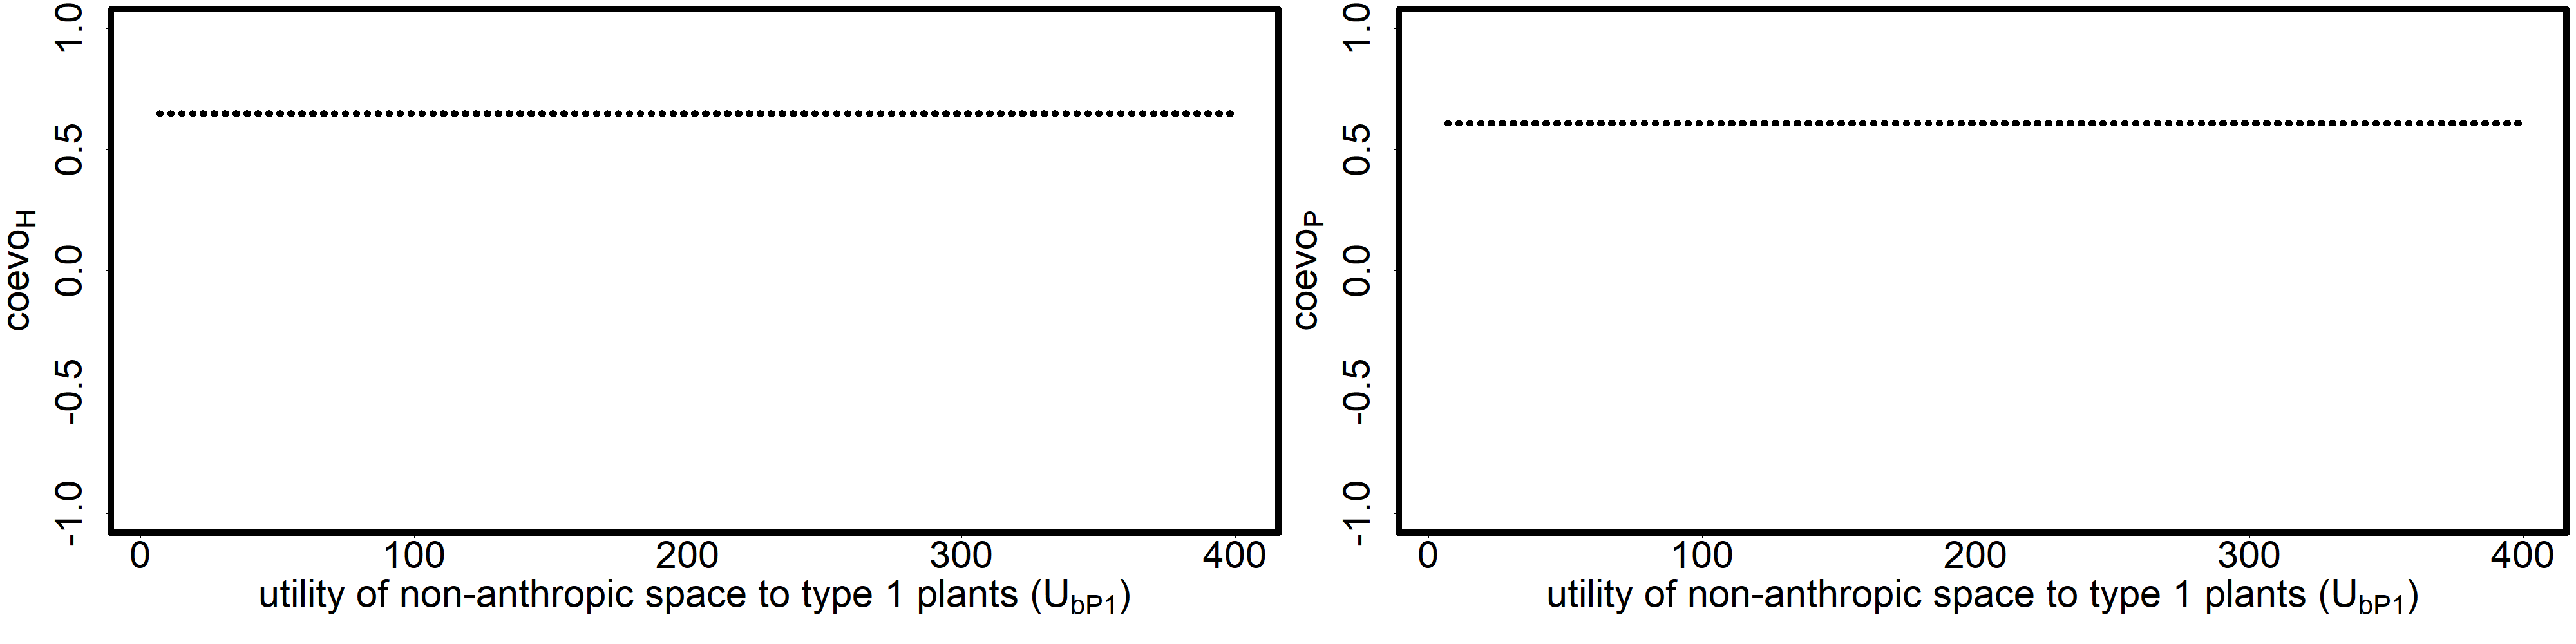
\includegraphics[width=1\linewidth]{plots/2_onePar-U.bP1_bifplot-pair}

\hypertarget{utility-of-other-resources-to-type-n-humans-u_bh_n}{%
\subsection{\texorpdfstring{utility \textbf{of} other resources \textbf{to} type n humans (\(U_{bH_{n}}\)):}{utility of other resources to type n humans (U\_\{bH\_\{n\}\}):}}\label{utility-of-other-resources-to-type-n-humans-u_bh_n}}

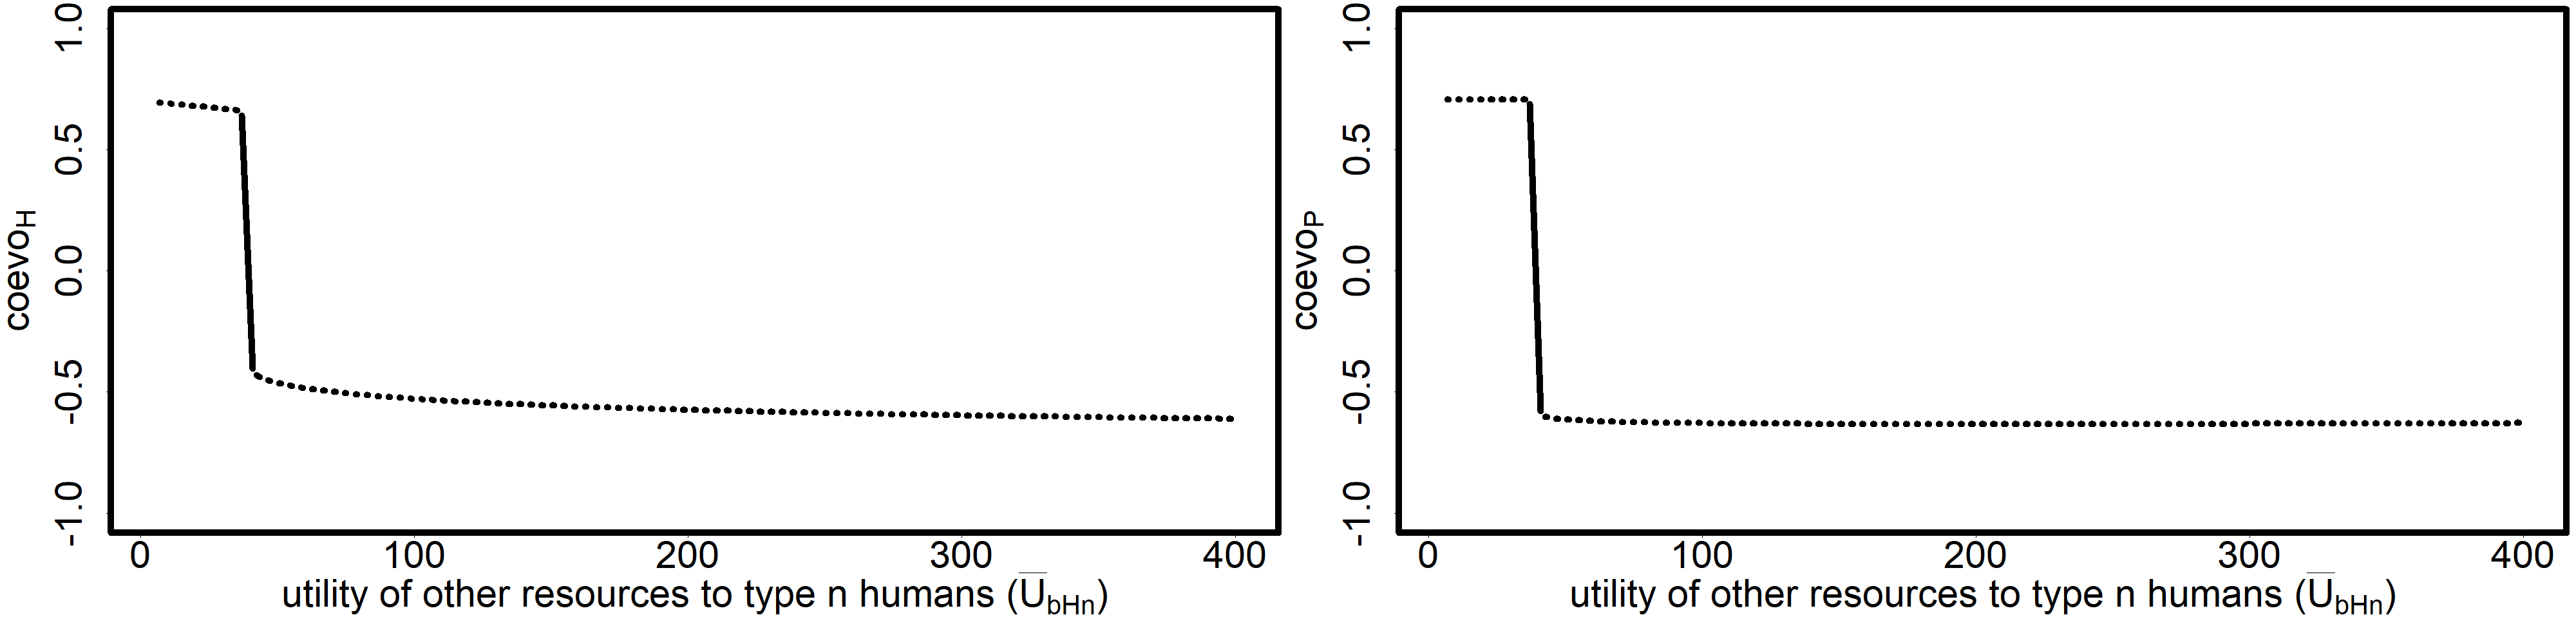
\includegraphics[width=1\linewidth]{plots/2_onePar-U.bHn_bifplot-pair}

\hypertarget{utility-of-non-anthropic-space-to-type-n-plants-u_bp_n}{%
\subsection{\texorpdfstring{utility \textbf{of} non-anthropic space \textbf{to} type n plants (\(U_{bP_{n}}\)):}{utility of non-anthropic space to type n plants (U\_\{bP\_\{n\}\}):}}\label{utility-of-non-anthropic-space-to-type-n-plants-u_bp_n}}

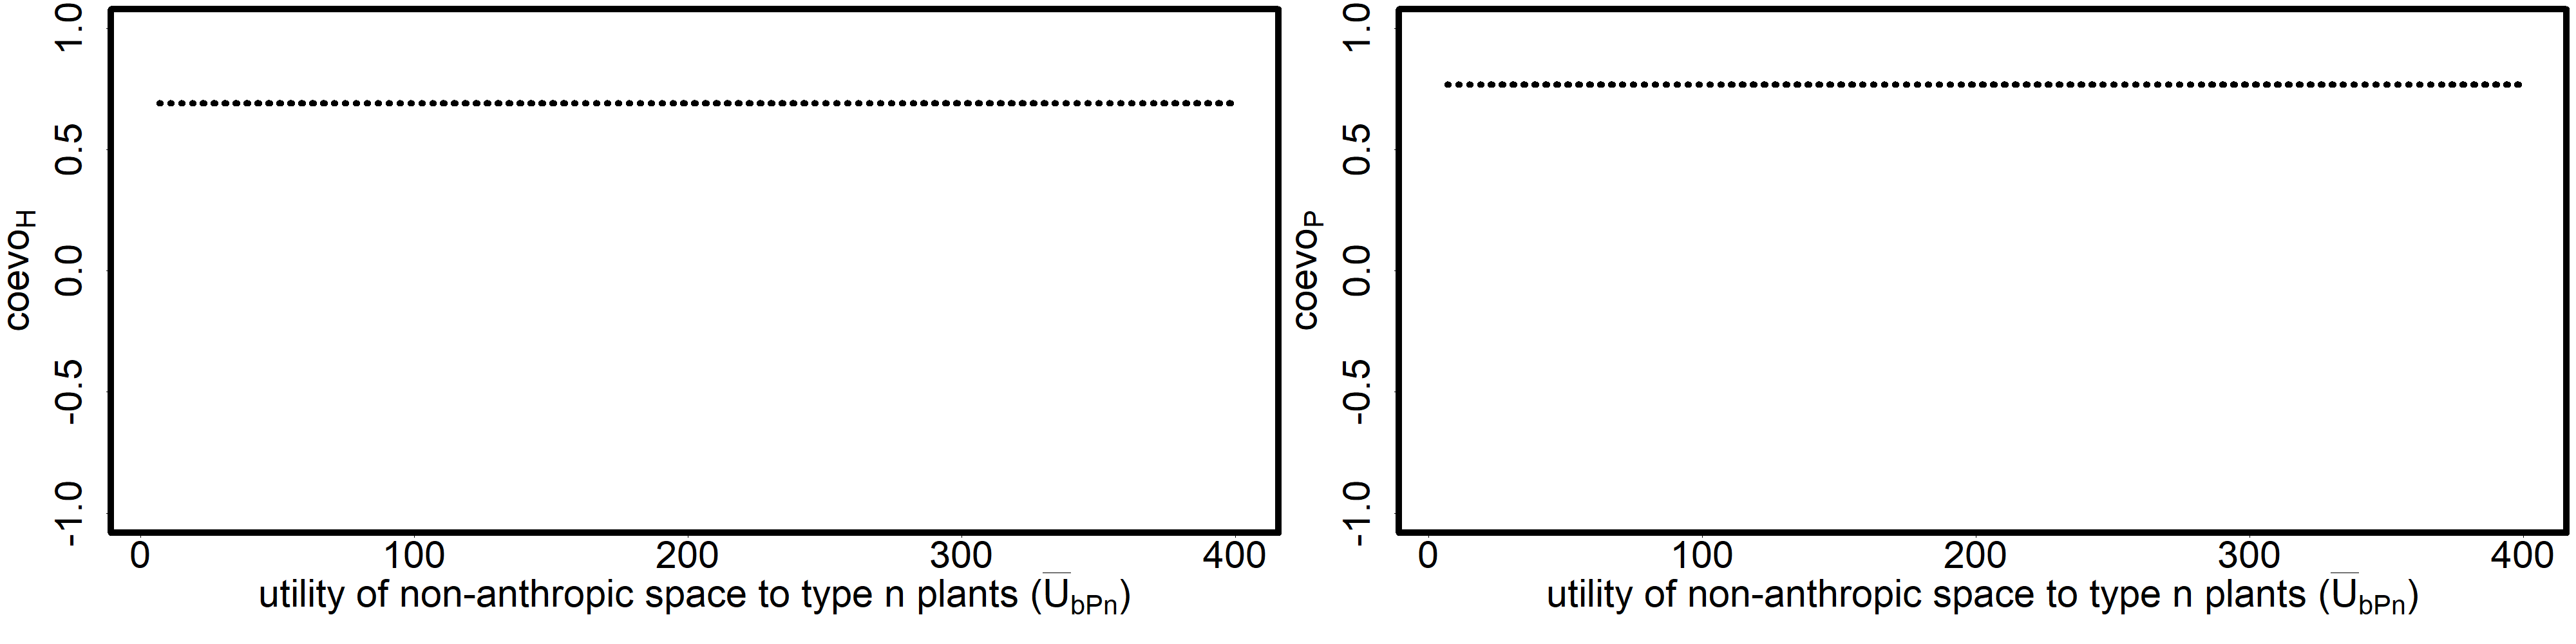
\includegraphics[width=1\linewidth]{plots/2_onePar-U.bPn_bifplot-pair}

\hypertarget{maximum-contiguous-area-to-be-used-by-plants-maxarea}{%
\subsection{\texorpdfstring{maximum contiguous area to be used by plants (\(MaxArea\)):}{maximum contiguous area to be used by plants (MaxArea):}}\label{maximum-contiguous-area-to-be-used-by-plants-maxarea}}

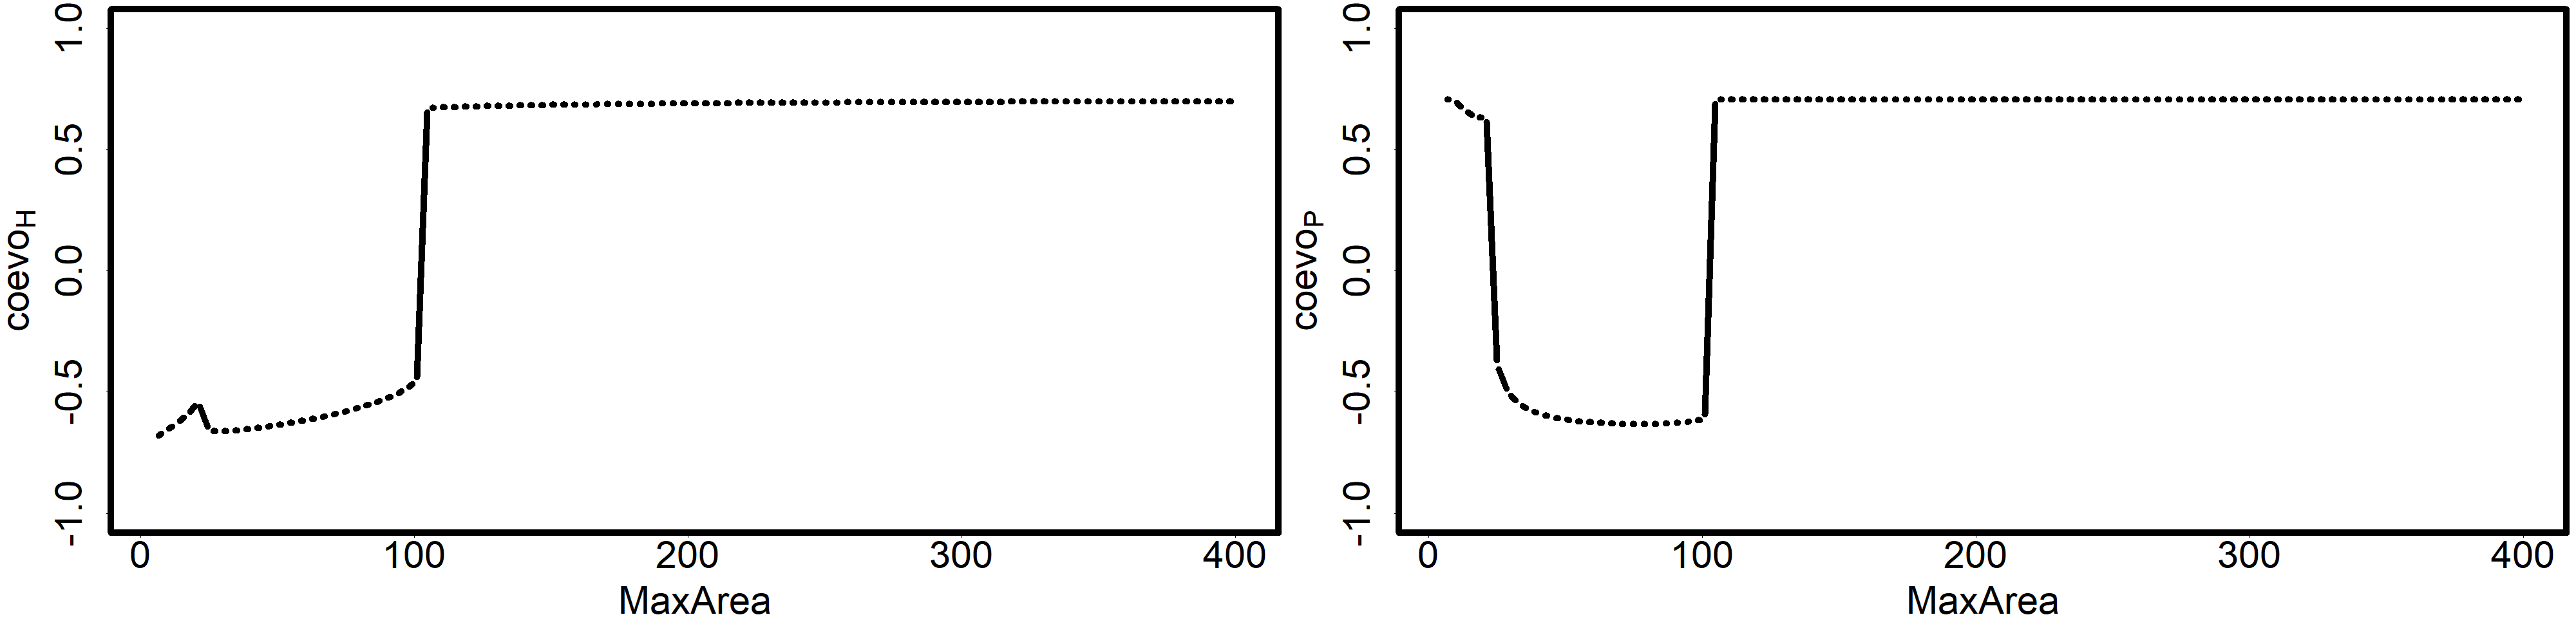
\includegraphics[width=1\linewidth]{plots/2_onePar-MaxArea_bifplot-pair}

\begin{center}\rule{0.5\linewidth}{0.5pt}\end{center}

\hypertarget{oscilations}{%
\section{Oscilations}\label{oscilations}}

Bifurcation plot with last 100 time steps (of 1000) to capture oscillations or `slow' asymptotic stability

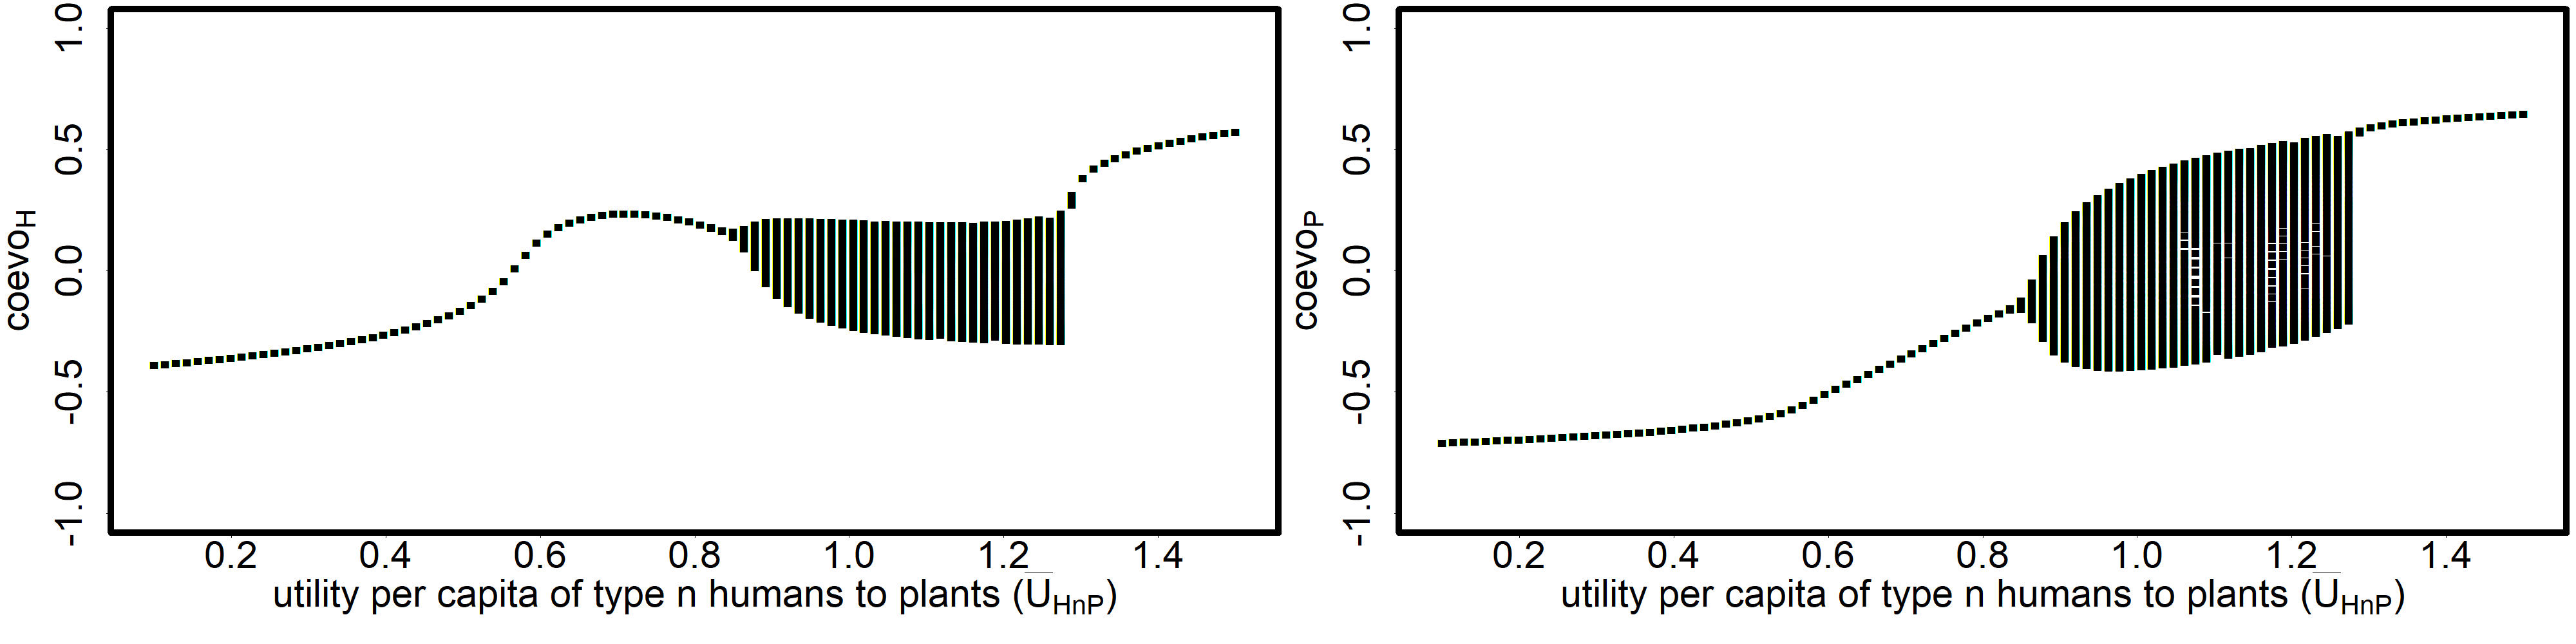
\includegraphics[width=1\linewidth]{plots/2_onePar-mU.HnP.osc_bifplot-pair}

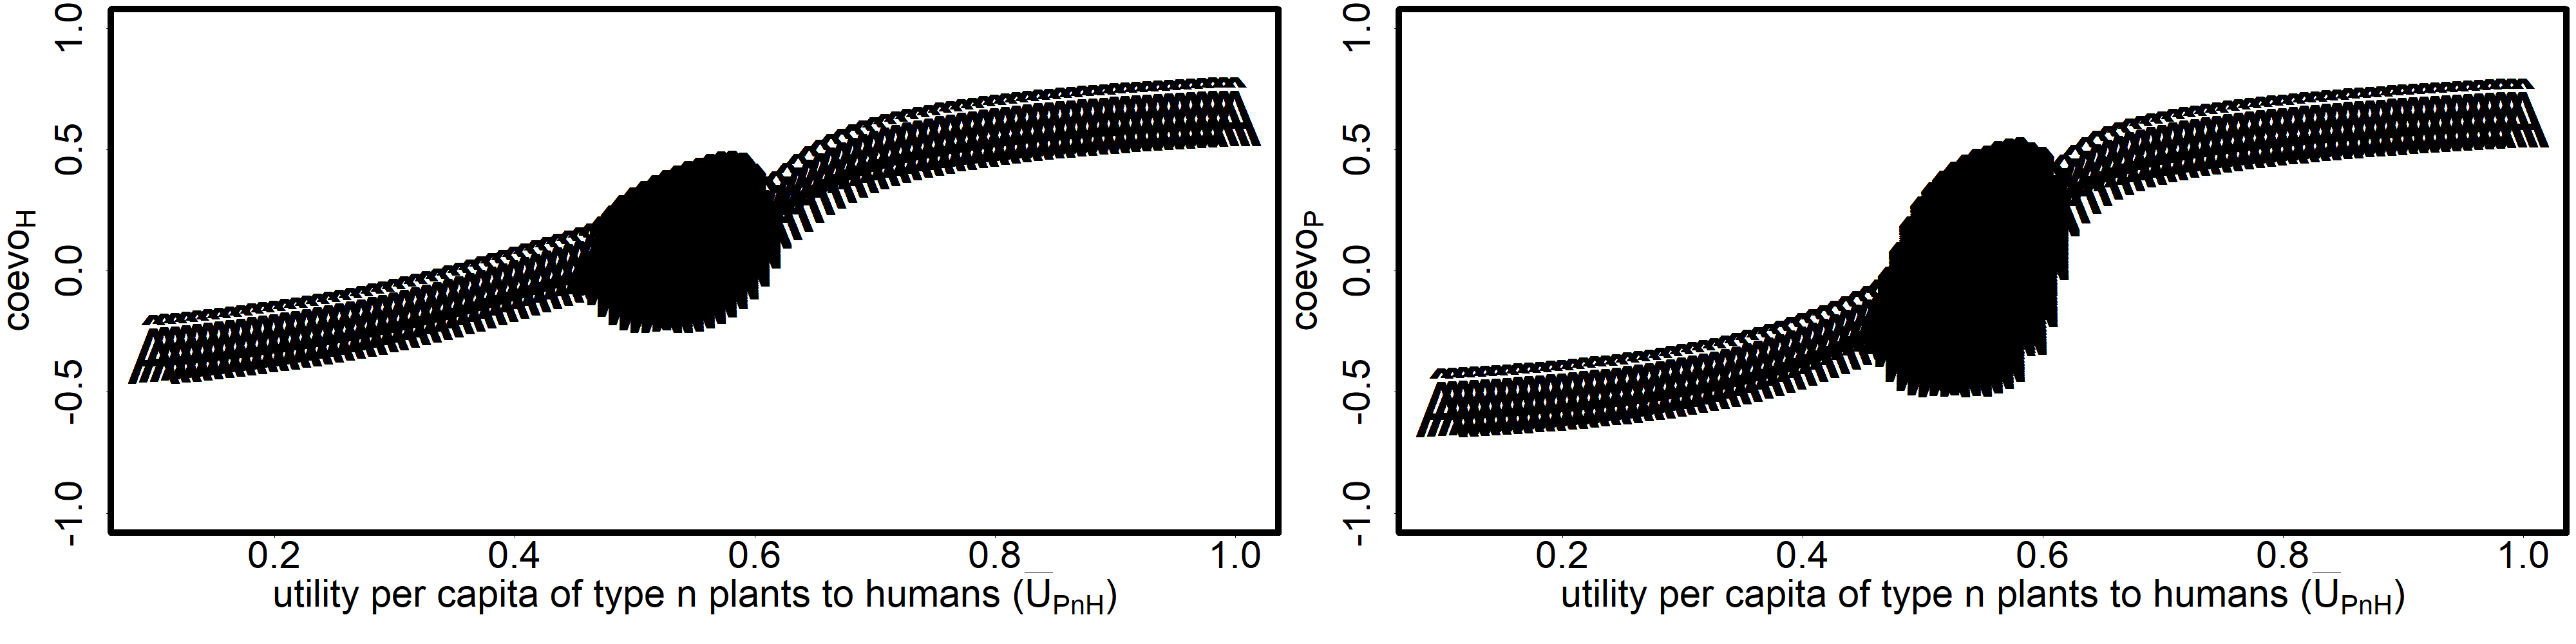
\includegraphics[width=1\linewidth]{plots/2_onePar-mU.PnH.osc_bifplot-pair}

\hypertarget{two-parameter-exploration}{%
\chapter{Two parameter exploration}\label{two-parameter-exploration}}

\newpage

\hypertarget{full-example}{%
\section{Full example}\label{full-example}}

\hypertarget{utility-per-capita-from-type-n-humans-and-plants-baru_h_np-x-baru_p_nh}{%
\subsection{\texorpdfstring{Utility per capita from type n humans and plants (\(\bar{U}_{H_{n}P}\) x \(\bar{U}_{P_{n}H}\))}{Utility per capita from type n humans and plants (\textbackslash bar\{U\}\_\{H\_\{n\}P\} x \textbackslash bar\{U\}\_\{P\_\{n\}H\})}}\label{utility-per-capita-from-type-n-humans-and-plants-baru_h_np-x-baru_p_nh}}

\sectionmark{$\bar{U}_{H_{n}P}$ x $\bar{U}_{P_{n}H}$}

\begin{table}[!h]

\caption{\label{tab:3mUHnPmUPnHtablepdf}Parameter setting}
\centering
\begin{tabular}[t]{l|l}
\hline
parameter & value\\
\hline
iniH & 10\\
\hline
iniP & 10\\
\hline
n.H & 30\\
\hline
n.P & 30\\
\hline
v.H & 0.15\\
\hline
v.P & 0.15\\
\hline
r.H & 0.04\\
\hline
r.P & 0.1\\
\hline
mU.PnH & 0 - 3 (sample = 15 )\\
\hline
mU.HnP & 0 - 3 (sample = 15 )\\
\hline
mU.P1H & 0.15\\
\hline
mU.H1P & 0\\
\hline
U.bHn & 10\\
\hline
U.bPn & 20\\
\hline
U.bH1 & 80\\
\hline
U.bP1 & 100\\
\hline
MaxArea & 200\\
\hline
\end{tabular}
\end{table}

\newpage

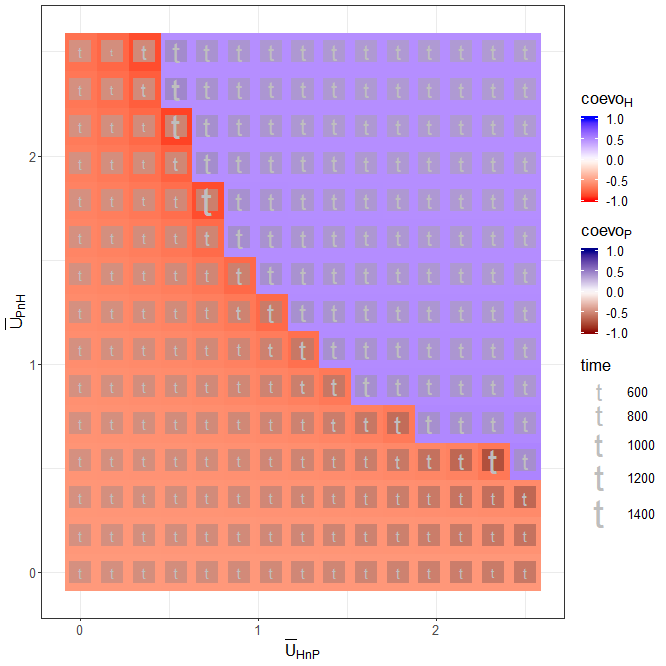
\includegraphics[width=1\linewidth]{plots/3_twoPar-mU.HnP-mU.PnH_plot}

\newpage

\hypertarget{exploration-on-default-setting-for-parameter-pairs}{%
\section{Exploration on `default' setting for parameter pairs}\label{exploration-on-default-setting-for-parameter-pairs}}

\hypertarget{number-of-types-of-humans-and-plants-n_h-x-n_p}{%
\subsection{\texorpdfstring{Number of types of humans and plants (\(n_{H}\) x \(n_{P}\))}{Number of types of humans and plants (n\_\{H\} x n\_\{P\})}}\label{number-of-types-of-humans-and-plants-n_h-x-n_p}}

\sectionmark{$n_{H}$ x $n_{P}$}

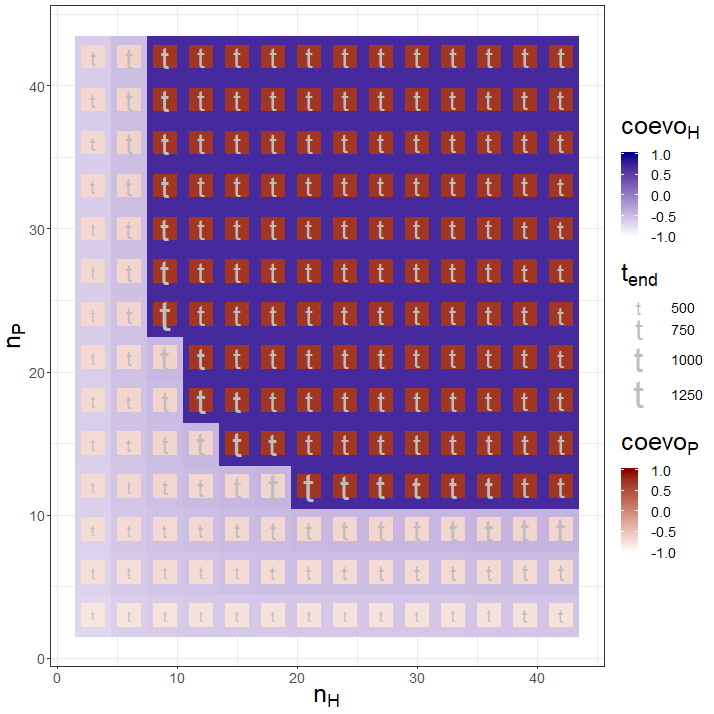
\includegraphics[width=1\linewidth]{plots/3_twoPar-n.H-n.P_plot}

\newpage

\hypertarget{undirected-variation-in-humans-and-plants-v_h-x-v_p}{%
\subsection{\texorpdfstring{Undirected variation in humans and plants (\(v_{H}\) x \(v_{P}\))}{Undirected variation in humans and plants (v\_\{H\} x v\_\{P\})}}\label{undirected-variation-in-humans-and-plants-v_h-x-v_p}}

\sectionmark{$v_{H}$ x $v_{P}$}

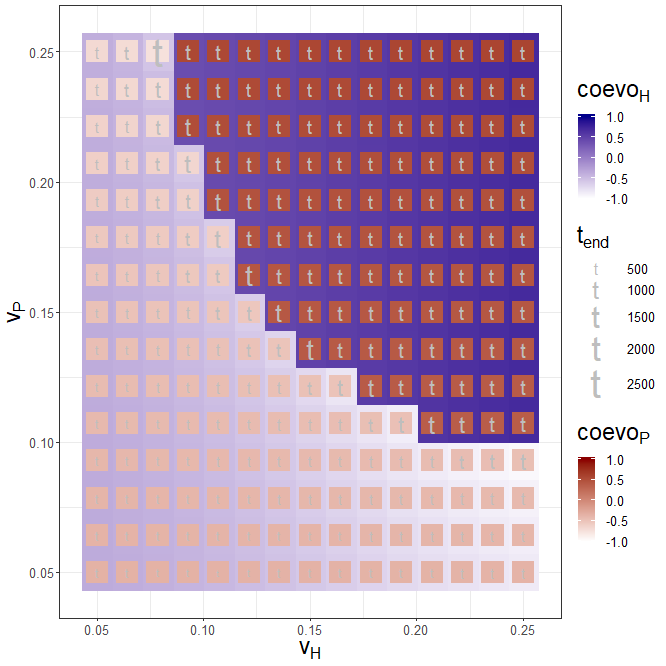
\includegraphics[width=1\linewidth]{plots/3_twoPar-v.H-v.P_plot}

\newpage

\hypertarget{utility-per-capita-from-type-1-humans-and-plants-baru_h_1p-x-baru_p_1h}{%
\subsection{\texorpdfstring{Utility per capita from type 1 humans and plants (\(\bar{U}_{H_{1}P}\) x \(\bar{U}_{P_{1}H}\))}{Utility per capita from type 1 humans and plants (\textbackslash bar\{U\}\_\{H\_\{1\}P\} x \textbackslash bar\{U\}\_\{P\_\{1\}H\})}}\label{utility-per-capita-from-type-1-humans-and-plants-baru_h_1p-x-baru_p_1h}}

\sectionmark{$\bar{U}_{H_{1}P}$ x $\bar{U}_{P_{1}H}$}

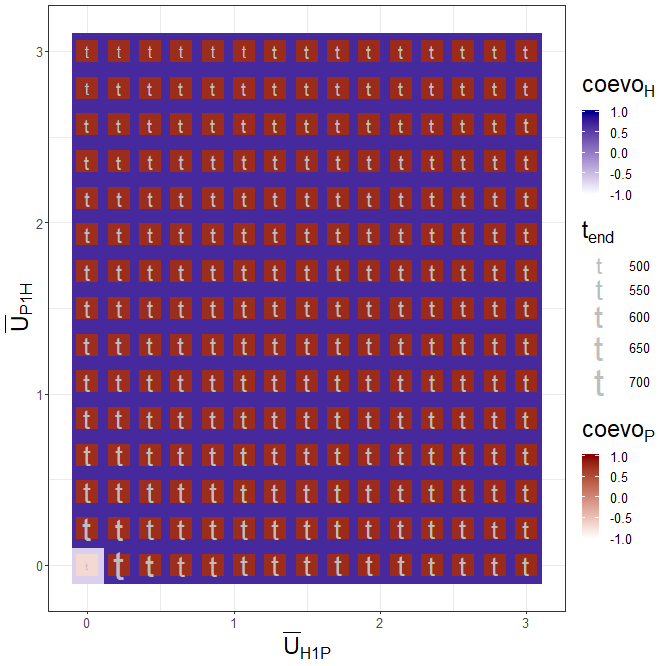
\includegraphics[width=1\linewidth]{plots/3_twoPar-mU.H1P-mU.P1H_plot}

\newpage

\hypertarget{utility-per-capita-from-type-n-humans-and-plants-baru_h_np-x-baru_p_nh-1}{%
\subsection{\texorpdfstring{Utility per capita from type n humans and plants (\(\bar{U}_{H_{n}P}\) x \(\bar{U}_{P_{n}H}\))}{Utility per capita from type n humans and plants (\textbackslash bar\{U\}\_\{H\_\{n\}P\} x \textbackslash bar\{U\}\_\{P\_\{n\}H\})}}\label{utility-per-capita-from-type-n-humans-and-plants-baru_h_np-x-baru_p_nh-1}}

\sectionmark{$\bar{U}_{H_{n}P}$ x $\bar{U}_{P_{n}H}$}

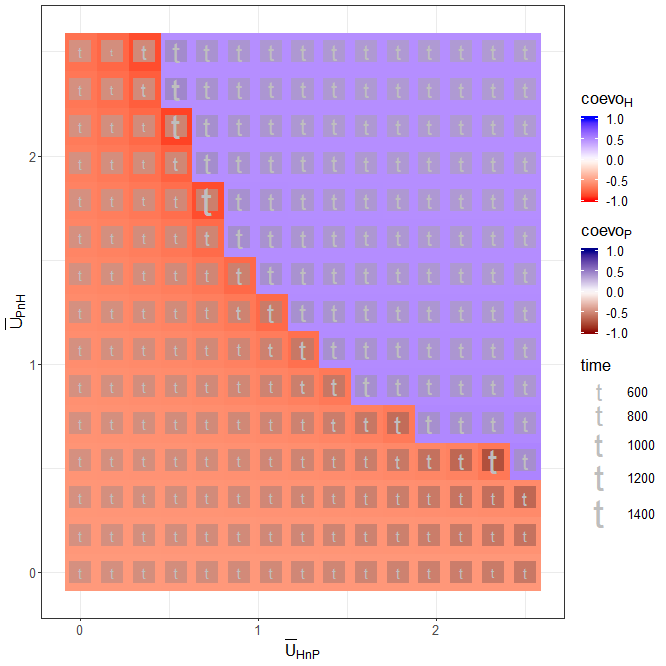
\includegraphics[width=1\linewidth]{plots/3_twoPar-mU.HnP-mU.PnH_plot}

\newpage

\hypertarget{utility-per-capita-from-humans-to-plants-baru_h_1p-x-baru_h_np}{%
\subsection{\texorpdfstring{Utility per capita from humans to plants (\(\bar{U}_{H_{1}P}\) x \(\bar{U}_{H_{n}P}\))}{Utility per capita from humans to plants (\textbackslash bar\{U\}\_\{H\_\{1\}P\} x \textbackslash bar\{U\}\_\{H\_\{n\}P\})}}\label{utility-per-capita-from-humans-to-plants-baru_h_1p-x-baru_h_np}}

\sectionmark{$\bar{U}_{H_{1}P}$ x $\bar{U}_{H_{n}P}$}

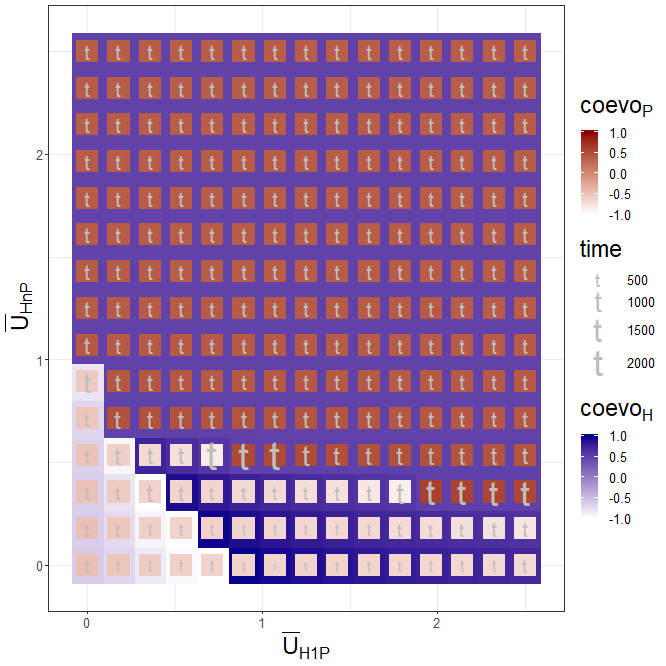
\includegraphics[width=1\linewidth]{plots/3_twoPar-mU.H1P-mU.HnP_plot}

\newpage

\hypertarget{utility-per-capita-from-plants-to-humans-baru_p_1h-x-baru_p_nh}{%
\subsection{\texorpdfstring{Utility per capita from plants to humans (\(\bar{U}_{P_{1}H}\) x \(\bar{U}_{P_{n}H}\))}{Utility per capita from plants to humans (\textbackslash bar\{U\}\_\{P\_\{1\}H\} x \textbackslash bar\{U\}\_\{P\_\{n\}H\})}}\label{utility-per-capita-from-plants-to-humans-baru_p_1h-x-baru_p_nh}}

\sectionmark{$\bar{U}_{P_{1}H}$ x $\bar{U}_{P_{n}H}$}

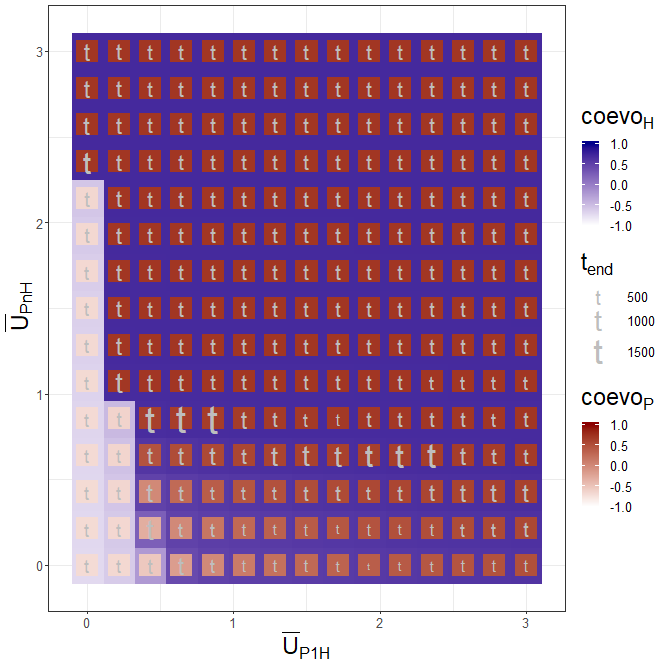
\includegraphics[width=1\linewidth]{plots/3_twoPar-mU.P1H-mU.PnH_plot}

\newpage

\hypertarget{utility-of-other-resources-to-type-1-humans-and-plants-u_bh_1-x-u_bp_1}{%
\subsection{\texorpdfstring{Utility of other resources to type 1 humans and plants (\(U_{bH_{1}}\) x \(U_{bP_{1}}\))}{Utility of other resources to type 1 humans and plants (U\_\{bH\_\{1\}\} x U\_\{bP\_\{1\}\})}}\label{utility-of-other-resources-to-type-1-humans-and-plants-u_bh_1-x-u_bp_1}}

\sectionmark{$U_{bH_{1}}$ x $U_{bP_{1}}$}

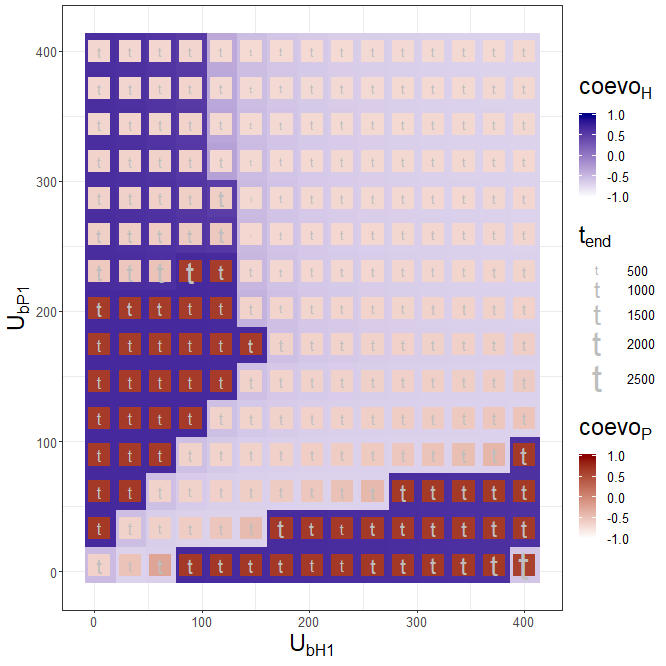
\includegraphics[width=1\linewidth]{plots/3_twoPar-U.bH1-U.bP1_plot}

\newpage

\hypertarget{utility-of-other-resources-to-type-n-humans-and-plants-u_bh_n-x-u_bp_n}{%
\subsection{\texorpdfstring{Utility of other resources to type n humans and plants (\(U_{bH_{n}}\) x \(U_{bP_{n}}\))}{Utility of other resources to type n humans and plants (U\_\{bH\_\{n\}\} x U\_\{bP\_\{n\}\})}}\label{utility-of-other-resources-to-type-n-humans-and-plants-u_bh_n-x-u_bp_n}}

\sectionmark{$U_{bH_{n}}$ x $U_{bP_{n}}$}

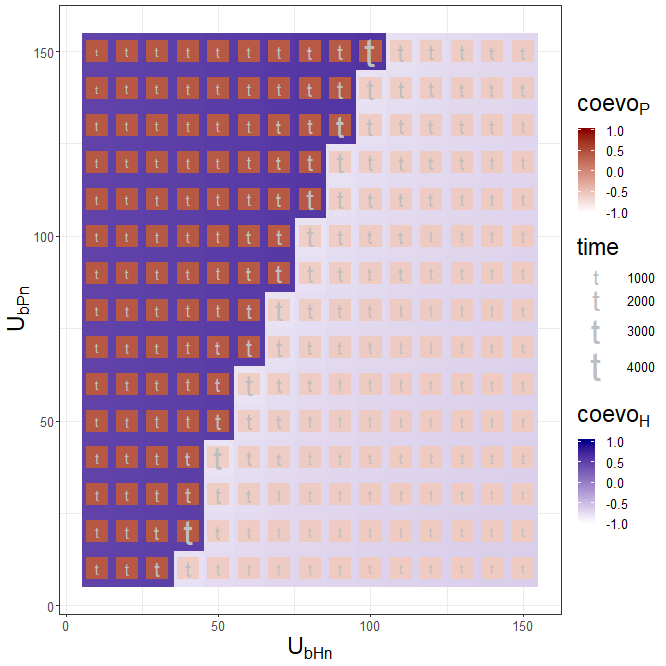
\includegraphics[width=1\linewidth]{plots/3_twoPar-U.bHn-U.bPn_plot}

\newpage

\hypertarget{utility-of-other-resources-to-humans-u_bh_1-x-u_bh_n}{%
\subsection{\texorpdfstring{Utility of other resources to humans (\(U_{bH_{1}}\) x \(U_{bH_{n}}\))}{Utility of other resources to humans (U\_\{bH\_\{1\}\} x U\_\{bH\_\{n\}\})}}\label{utility-of-other-resources-to-humans-u_bh_1-x-u_bh_n}}

\sectionmark{$U_{bH_{1}}$ x $U_{bH_{n}}$}

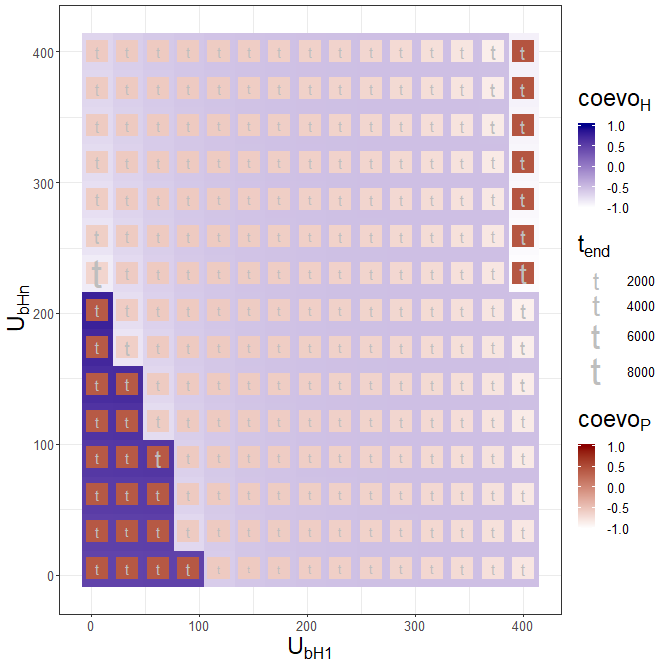
\includegraphics[width=1\linewidth]{plots/3_twoPar-U.bH1-U.bHn_plot}

\newpage

\hypertarget{utility-of-other-resources-to-plants-u_bp_1-x-u_bp_n}{%
\subsection{\texorpdfstring{Utility of other resources to plants (\(U_{bP_{1}}\) x \(U_{bP_{n}}\))}{Utility of other resources to plants (U\_\{bP\_\{1\}\} x U\_\{bP\_\{n\}\})}}\label{utility-of-other-resources-to-plants-u_bp_1-x-u_bp_n}}

\sectionmark{$U_{bP_{1}}$ x $U_{bP_{n}}$}

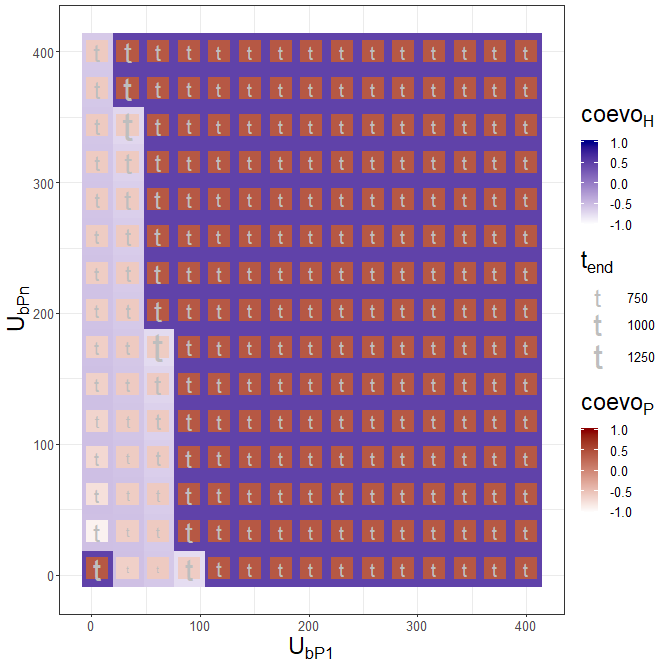
\includegraphics[width=1\linewidth]{plots/3_twoPar-U.bP1-U.bPn_plot}

\hypertarget{utility-of-other-resources-to-type-1-humans-and-utility-per-capita-of-type-1-humans-to-plants-u_bh_1-x-baru_h_1p}{%
\subsection{\texorpdfstring{Utility of other resources to type 1 humans and utility per capita of type 1 humans to plants (\(U_{bH_{1}}\) x \(\bar{U}_{H_{1}P}\))}{Utility of other resources to type 1 humans and utility per capita of type 1 humans to plants (U\_\{bH\_\{1\}\} x \textbackslash bar\{U\}\_\{H\_\{1\}P\})}}\label{utility-of-other-resources-to-type-1-humans-and-utility-per-capita-of-type-1-humans-to-plants-u_bh_1-x-baru_h_1p}}

\sectionmark{$U_{bH_{1}}$ x $\bar{U}_{H_{1}P}$}

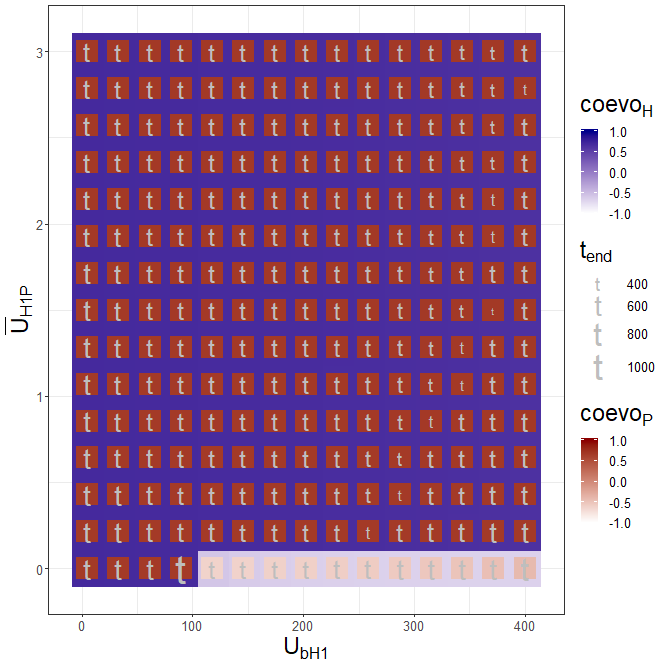
\includegraphics[width=1\linewidth]{plots/3_twoPar-U.bH1-mU.H1P_plot}

\newpage

\hypertarget{utility-of-other-resources-to-type-1-plants-and-utility-per-capita-of-type-1-plants-to-humans-u_bp_1-x-baru_p_1h}{%
\subsection{\texorpdfstring{Utility of other resources to type 1 plants and utility per capita of type 1 plants to humans (\(U_{bP_{1}}\) x \(\bar{U}_{P_{1}H}\))}{Utility of other resources to type 1 plants and utility per capita of type 1 plants to humans (U\_\{bP\_\{1\}\} x \textbackslash bar\{U\}\_\{P\_\{1\}H\})}}\label{utility-of-other-resources-to-type-1-plants-and-utility-per-capita-of-type-1-plants-to-humans-u_bp_1-x-baru_p_1h}}

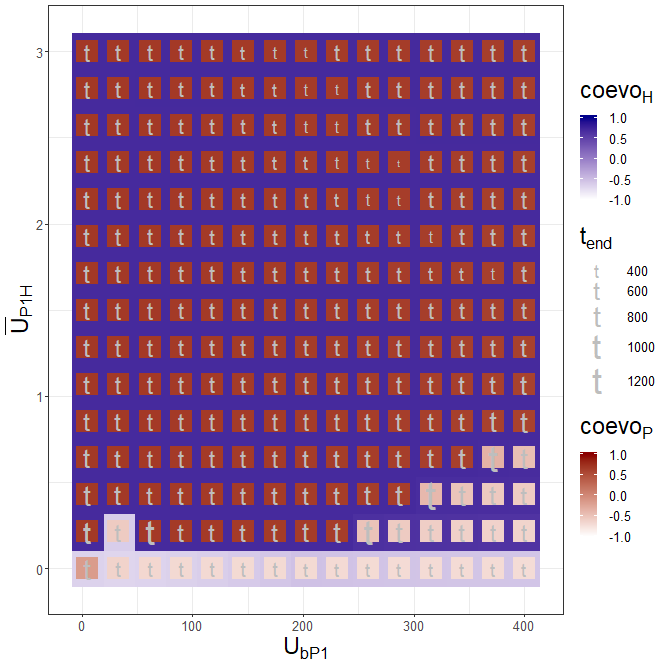
\includegraphics[width=1\linewidth]{plots/3_twoPar-U.bP1-mU.P1H_plot}

\newpage

\hypertarget{utility-of-other-resources-to-type-n-humans-and-utility-per-capita-of-type-n-humans-to-plants-u_bh_n-x-baru_h_np}{%
\subsection{\texorpdfstring{Utility of other resources to type n humans and utility per capita of type n humans to plants (\(U_{bH_{n}}\) x \(\bar{U}_{H_{n}P}\))}{Utility of other resources to type n humans and utility per capita of type n humans to plants (U\_\{bH\_\{n\}\} x \textbackslash bar\{U\}\_\{H\_\{n\}P\})}}\label{utility-of-other-resources-to-type-n-humans-and-utility-per-capita-of-type-n-humans-to-plants-u_bh_n-x-baru_h_np}}

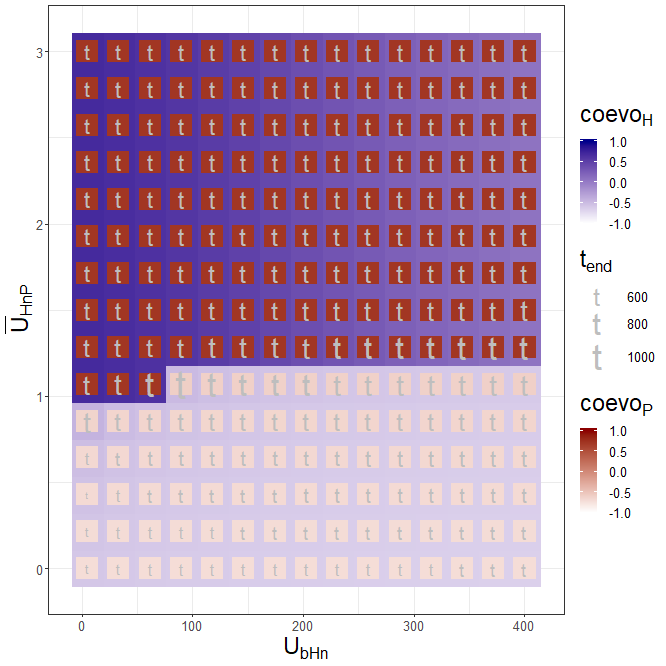
\includegraphics[width=1\linewidth]{plots/3_twoPar-U.bHn-mU.HnP_plot}

\newpage

\hypertarget{utility-of-other-resources-to-type-n-plants-and-utility-per-capita-of-type-n-plants-to-humans-u_bp_n-x-baru_p_nh}{%
\subsection{\texorpdfstring{Utility of other resources to type n plants and utility per capita of type n plants to humans (\(U_{bP_{n}}\) x \(\bar{U}_{P_{n}H}\))}{Utility of other resources to type n plants and utility per capita of type n plants to humans (U\_\{bP\_\{n\}\} x \textbackslash bar\{U\}\_\{P\_\{n\}H\})}}\label{utility-of-other-resources-to-type-n-plants-and-utility-per-capita-of-type-n-plants-to-humans-u_bp_n-x-baru_p_nh}}

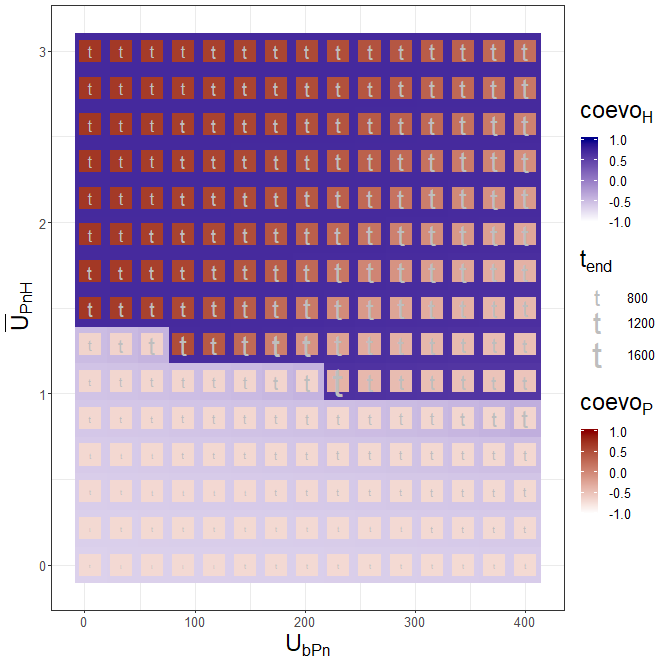
\includegraphics[width=1\linewidth]{plots/3_twoPar-U.bPn-mU.PnH_plot}

\newpage

\hypertarget{four-parameter-exploration}{%
\chapter{Four parameter exploration}\label{four-parameter-exploration}}

\newpage

\hypertarget{number-of-types-and-undirected-variation-of-humans-and-plants-n_h-x-n_p-x-v_h-x-v_p}{%
\section{\texorpdfstring{Number of types and undirected variation of humans and plants (\(n_{H}\) x \(n_{P}\) x \(v_{H}\) x \(v_{P}\))}{Number of types and undirected variation of humans and plants (n\_\{H\} x n\_\{P\} x v\_\{H\} x v\_\{P\})}}\label{number-of-types-and-undirected-variation-of-humans-and-plants-n_h-x-n_p-x-v_h-x-v_p}}

\sectionmark{$n_{H}$ x $n_{P}$ x $v_{H}$ x $v_{P}$}

\begin{table}[!h]

\caption{\label{tab:4nvtablepdf}Parameter setting}
\centering
\begin{tabular}[t]{l|l}
\hline
parameter & value\\
\hline
iniH & 10\\
\hline
iniP & 10\\
\hline
n.H & 5 - 45 (sample = 5 )\\
\hline
n.P & 5 - 45 (sample = 5 )\\
\hline
v.H & 0.05 - 0.25 (sample = 5 )\\
\hline
v.P & 0.05 - 0.25 (sample = 5 )\\
\hline
r.H & 0.04\\
\hline
r.P & 0.1\\
\hline
mU.PnH & 1.5\\
\hline
mU.HnP & 1\\
\hline
mU.P1H & 0.15\\
\hline
mU.H1P & 0\\
\hline
U.bHn & 10\\
\hline
U.bPn & 20\\
\hline
U.bH1 & 80\\
\hline
U.bP1 & 100\\
\hline
MaxArea & 200\\
\hline
\end{tabular}
\end{table}

\newpage

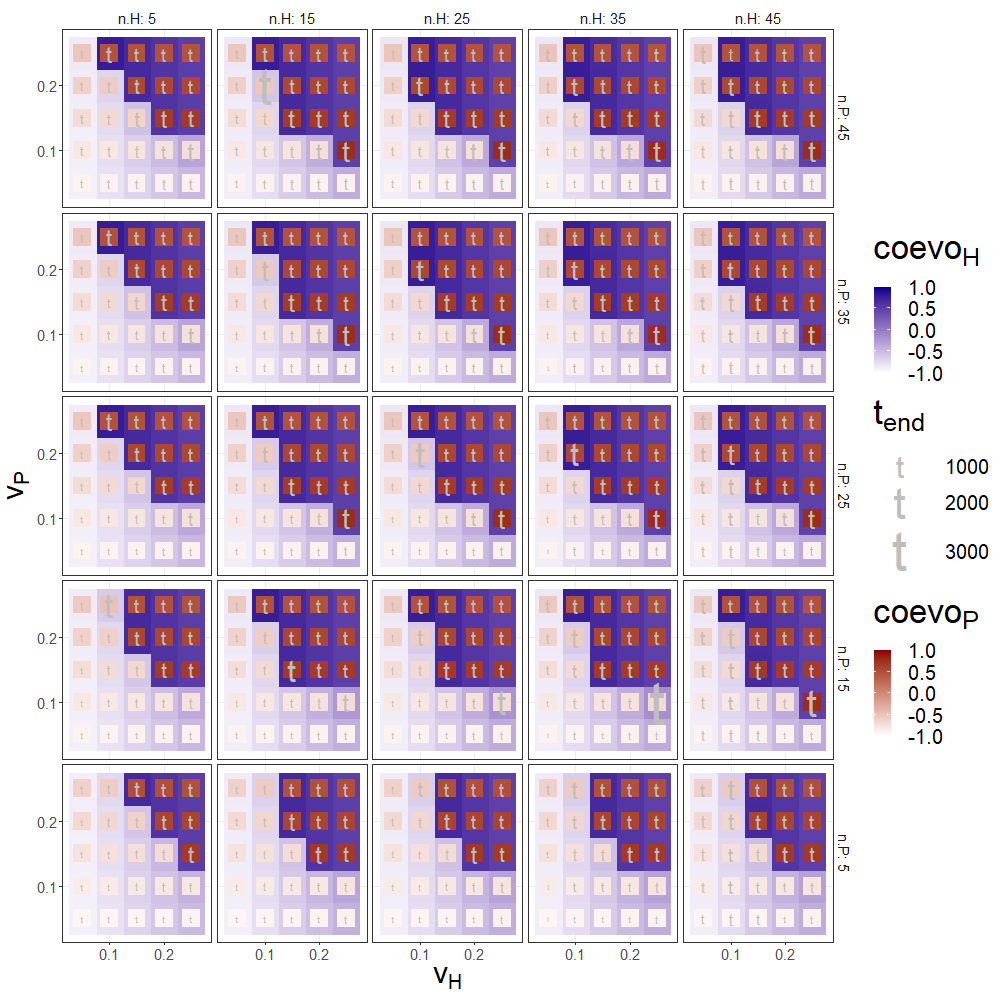
\includegraphics[width=1\linewidth]{plots/4_fourPar-n-v_plot}

\textbf{\emph{Interpretation}}:\\
- Higher values of all four parameters facilitate coevolution. Undirected variation has a stronger effect than number of types.
- As a summary of possible end-states:\\
+ \emph{`Fast' coevolution} (red square in blue tile, small \emph{t}): most cases when the numbers of types (\(n_{H}\), \(n_{P}\)) are greater than \textbf{15} and values of undirected variation (\(v_{H}\), \(v_{P}\)) higher than \textbf{0.15}.\\
+ \emph{`Semi-domestication' without cultivation} (redish square in whitish tile): cases when \(v_{P}\geq 0.15\) and \(v_{H}\leq 0.15\).\\
+ \emph{`Semi-cultivation' without domestication} (whitish square in blue tile): cases when \(v_{H}\geq 0.15\) and \(v_{P}\leq 0.15\).

\newpage

\hypertarget{utility-per-capita-between-humans-and-plants-baru_h_1p-x-baru_p_1h-x-baru_h_np-x-baru_p_nh}{%
\section{\texorpdfstring{Utility per capita between humans and plants (\(\bar{U}_{H_{1}P}\) x \(\bar{U}_{P_{1}H}\) x \(\bar{U}_{H_{n}P}\) x \(\bar{U}_{P_{n}H}\))}{Utility per capita between humans and plants (\textbackslash bar\{U\}\_\{H\_\{1\}P\} x \textbackslash bar\{U\}\_\{P\_\{1\}H\} x \textbackslash bar\{U\}\_\{H\_\{n\}P\} x \textbackslash bar\{U\}\_\{P\_\{n\}H\})}}\label{utility-per-capita-between-humans-and-plants-baru_h_1p-x-baru_p_1h-x-baru_h_np-x-baru_p_nh}}

\sectionmark{$\bar{U}_{H_{1}P}$ x $\bar{U}_{P_{1}H}$ x $\bar{U}_{H_{n}P}$ x $\bar{U}_{P_{n}H}$}

\begin{table}[!h]

\caption{\label{tab:4mUHPmUPHtablepdf}Parameter setting}
\centering
\begin{tabular}[t]{l|l}
\hline
parameter & value\\
\hline
iniH & 10\\
\hline
iniP & 10\\
\hline
n.H & 30\\
\hline
n.P & 30\\
\hline
v.H & 0.15\\
\hline
v.P & 0.15\\
\hline
r.H & 0.04\\
\hline
r.P & 0.1\\
\hline
mU.PnH & 0 - 3 (sample = 5 )\\
\hline
mU.HnP & 0 - 3 (sample = 5 )\\
\hline
mU.P1H & 0 - 3 (sample = 5 )\\
\hline
mU.H1P & 0 - 3 (sample = 5 )\\
\hline
U.bHn & 10\\
\hline
U.bPn & 20\\
\hline
U.bH1 & 80\\
\hline
U.bP1 & 100\\
\hline
MaxArea & 200\\
\hline
\end{tabular}
\end{table}

\newpage

\includegraphics[width=1\linewidth]{plots/4_fourPar-mU.HP-mU.PH_plot}

\textbf{\emph{Interpretation}}:\\
- Higher values of all four parameters facilitate coevolution; under the `default' setting, a value around 1 is enough for all four parameters (intermediate values in this exploration).\\
- Coevolution is still possible if any single one of these parameters equal zero (first rows or first columns). Under this type of conditions, cultivation (blue) is more probable than domestication (red), and the latter is strongly dependent on a non-null \(\bar{U}_{H_{n}P}\).\\
- As a summary of possible end-states:\\
+ \emph{`Fast' coevolution} (red square in blue tile, small \emph{t}): most cases when values are greater than 0.75.\\
+ \emph{Domestication without cultivation} (red square in whitish tile): most cases when \(\bar{U}_{H_{n}P}>0.75\), \(\bar{U}_{H_{1}P}\geq 0.75\), \(\bar{U}_{P_{n}H}=0\), and \(\bar{U}_{P_{1}H}<2\).\\
+ \emph{Cultivation without domestication} (whitish square in blue tile): most cases when \(\bar{U}_{H_{n}P} = 0\).

\newpage

\hypertarget{utility-from-other-resources-to-humans-and-plants-u_bh_1-x-u_bp_1-x-u_bh_n-x-u_bp_n}{%
\section{\texorpdfstring{Utility from other resources to humans and plants (\(U_{bH_{1}}\) x \(U_{bP_{1}}\) x \(U_{bH_{n}}\) x \(U_{bP_{n}}\))}{Utility from other resources to humans and plants (U\_\{bH\_\{1\}\} x U\_\{bP\_\{1\}\} x U\_\{bH\_\{n\}\} x U\_\{bP\_\{n\}\})}}\label{utility-from-other-resources-to-humans-and-plants-u_bh_1-x-u_bp_1-x-u_bh_n-x-u_bp_n}}

\sectionmark{$U_{bH_{1}}$ x $U_{bP_{1}}$ x $U_{bH_{n}}$ x $U_{bP_{n}}$}

For this experiment, consider that the default setting includes \(MaxArea=200\) (i.e.~the maximum for the plant population).

\begin{table}[!h]

\caption{\label{tab:4UbHUbPtablepdf}Parameter setting}
\centering
\begin{tabular}[t]{l|l}
\hline
parameter & value\\
\hline
iniH & 10\\
\hline
iniP & 10\\
\hline
n.H & 30\\
\hline
n.P & 30\\
\hline
v.H & 0.15\\
\hline
v.P & 0.15\\
\hline
r.H & 0.04\\
\hline
r.P & 0.1\\
\hline
mU.PnH & 1.5\\
\hline
mU.HnP & 1\\
\hline
mU.P1H & 0.15\\
\hline
mU.H1P & 0\\
\hline
U.bHn & 5 - 300 (sample = 5 )\\
\hline
U.bPn & 5 - 300 (sample = 5 )\\
\hline
U.bH1 & 5 - 300 (sample = 5 )\\
\hline
U.bP1 & 5 - 300 (sample = 5 )\\
\hline
MaxArea & 200\\
\hline
\end{tabular}
\end{table}

\newpage

\includegraphics[width=1\linewidth]{plots/4_fourPar-U.bH-U.bP_plot}

\textbf{\emph{Interpretation}}:\\
- Lower values of the two human-related parameters (\(U_{bH_{1}}\), \(U_{bH_{n}}\)) facilitate coevolution; under the `default' setting and for all four parameters, values greater or equal to \(MaxArea\) (here, 200) impede coevolution. Inversely, higher values of the plant-related parameters (\(U_{bP_{1}}\), \(U_{bP_{n}}\)) facilitate coevolution. The human-related parameters, together regulating the scale of the subsistence alternatives for humans, are significantly more important; their relationship (if one is greater than the other) seems to be less important as long as their combined sum is small enough.\\
- Coevolution is likely to occur when \(U_{bH_{1}}=5\) (first row in small grids), unless \(U_{bH_{n}}\) is too big and \(U_{bP_{1}}\) is too small.\\
- As a summary of possible end-states:\\
+ \emph{`Fast' coevolution} (red square in blue tile, small \emph{t}): most cases when \(U_{bH_{1}}\) and \(U_{bH_{n}}<153\).\\
+ \emph{Domestication without cultivation} (red square in whitish tile): most cases when \(U_{bP_{n}}=5\), \(U_{bP_{1}}=5\) (i.e.~there is very little carrying capacity for plants beyond the anthropic space) and \(U_{bH_{1}}>5\) (i.e.~humans get enough of other resources when -still- not engaged in agriculture).\\
+ \emph{Cultivation without domestication} (whitish square in blue tile): \emph{no cases are visible under these conditions}.

\newpage

\hypertarget{utility-from-other-resources-to-humans-and-utility-per-capita-of-plants-to-humans-u_bh_1-x-u_bh_n-x-baru_p_1h-x-baru_p_nh}{%
\section{\texorpdfstring{Utility from other resources to humans and utility per capita of plants to humans (\(U_{bH_{1}}\) x \(U_{bH_{n}}\) x \(\bar{U}_{P_{1}H}\) x \(\bar{U}_{P_{n}H}\))}{Utility from other resources to humans and utility per capita of plants to humans (U\_\{bH\_\{1\}\} x U\_\{bH\_\{n\}\} x \textbackslash bar\{U\}\_\{P\_\{1\}H\} x \textbackslash bar\{U\}\_\{P\_\{n\}H\})}}\label{utility-from-other-resources-to-humans-and-utility-per-capita-of-plants-to-humans-u_bh_1-x-u_bh_n-x-baru_p_1h-x-baru_p_nh}}

\sectionmark{$U_{bH_{1}}$ x $U_{bH_{n}}$ x $\bar{U}_{P_{1}H}$ x $\bar{U}_{P_{n}H}$}

All four parameters affect directly the carrying capacity for humans.

\begin{table}[!h]

\caption{\label{tab:4UbHUPHtablepdf}Parameter setting}
\centering
\begin{tabular}[t]{l|l}
\hline
parameter & value\\
\hline
iniH & 10\\
\hline
iniP & 10\\
\hline
n.H & 30\\
\hline
n.P & 30\\
\hline
v.H & 0.15\\
\hline
v.P & 0.15\\
\hline
r.H & 0.04\\
\hline
r.P & 0.1\\
\hline
mU.PnH & 0 - 3 (sample = 5 )\\
\hline
mU.HnP & 1\\
\hline
mU.P1H & 0 - 3 (sample = 5 )\\
\hline
mU.H1P & 0\\
\hline
U.bHn & 5 - 300 (sample = 5 )\\
\hline
U.bPn & 20\\
\hline
U.bH1 & 5 - 300 (sample = 5 )\\
\hline
U.bP1 & 100\\
\hline
MaxArea & 200\\
\hline
\end{tabular}
\end{table}

\newpage

\includegraphics[width=1\linewidth]{plots/4_fourPar-U.bH-U.PH_plot}

\newpage

\hypertarget{utility-from-other-resources-to-plants-and-utility-per-capita-of-humans-to-plants-u_bp_1-x-u_bp_n-x-baru_h_1p-x-baru_h_np}{%
\section{\texorpdfstring{Utility from other resources to plants and utility per capita of humans to plants (\(U_{bP_{1}}\) x \(U_{bP_{n}}\) x \(\bar{U}_{H_{1}P}\) x \(\bar{U}_{H_{n}P}\))}{Utility from other resources to plants and utility per capita of humans to plants (U\_\{bP\_\{1\}\} x U\_\{bP\_\{n\}\} x \textbackslash bar\{U\}\_\{H\_\{1\}P\} x \textbackslash bar\{U\}\_\{H\_\{n\}P\})}}\label{utility-from-other-resources-to-plants-and-utility-per-capita-of-humans-to-plants-u_bp_1-x-u_bp_n-x-baru_h_1p-x-baru_h_np}}

\sectionmark{$U_{bP_{1}}$ x $U_{bP_{n}}$ x $\bar{U}_{H_{1}P}$ x $\bar{U}_{H_{n}P}$}

All four parameters affect directly the carrying capacity for plants.

\begin{table}[!h]

\caption{\label{tab:4UbPUHPtablepdf}Parameter setting}
\centering
\begin{tabular}[t]{l|l}
\hline
parameter & value\\
\hline
iniH & 10\\
\hline
iniP & 10\\
\hline
n.H & 30\\
\hline
n.P & 30\\
\hline
v.H & 0.15\\
\hline
v.P & 0.15\\
\hline
r.H & 0.04\\
\hline
r.P & 0.1\\
\hline
mU.PnH & 1.5\\
\hline
mU.HnP & 0 - 3 (sample = 5 )\\
\hline
mU.P1H & 0.15\\
\hline
mU.H1P & 0 - 3 (sample = 5 )\\
\hline
U.bHn & 10\\
\hline
U.bPn & 5 - 300 (sample = 5 )\\
\hline
U.bH1 & 80\\
\hline
U.bP1 & 5 - 300 (sample = 5 )\\
\hline
MaxArea & 200\\
\hline
\end{tabular}
\end{table}

\newpage

\includegraphics[width=1\linewidth]{plots/4_fourPar-U.bP-mU.HP_plot}

\newpage

\hypertarget{utility-from-other-resources-and-utility-per-capita-of-type-1-humans-and-plants-u_bp_1-x-u_bh_1-x-baru_h_1p-x-baru_p_1h}{%
\section{\texorpdfstring{Utility from other resources and utility per capita of type 1 humans and plants (\(U_{bP_{1}}\) x \(U_{bH_{1}}\) x \(\bar{U}_{H_{1}P}\) x \(\bar{U}_{P_{1}H}\))}{Utility from other resources and utility per capita of type 1 humans and plants (U\_\{bP\_\{1\}\} x U\_\{bH\_\{1\}\} x \textbackslash bar\{U\}\_\{H\_\{1\}P\} x \textbackslash bar\{U\}\_\{P\_\{1\}H\})}}\label{utility-from-other-resources-and-utility-per-capita-of-type-1-humans-and-plants-u_bp_1-x-u_bh_1-x-baru_h_1p-x-baru_p_1h}}

\sectionmark{$U_{bP_{1}}$ x $U_{bH_{1}}$ x $\bar{U}_{H_{1}P}$ x $\bar{U}_{P_{1}H}$}

This exploration reflects the state at the start of simulations (both populations are mostly of type 1).

\begin{table}[!h]

\caption{\label{tab:4Ub1mU1tablepdf}Parameter setting}
\centering
\begin{tabular}[t]{l|l}
\hline
parameter & value\\
\hline
iniH & 10\\
\hline
iniP & 10\\
\hline
n.H & 30\\
\hline
n.P & 30\\
\hline
v.H & 0.15\\
\hline
v.P & 0.15\\
\hline
r.H & 0.04\\
\hline
r.P & 0.1\\
\hline
mU.PnH & 1.5\\
\hline
mU.HnP & 1\\
\hline
mU.P1H & 0 - 3 (sample = 5 )\\
\hline
mU.H1P & 0 - 3 (sample = 5 )\\
\hline
U.bHn & 10\\
\hline
U.bPn & 20\\
\hline
U.bH1 & 5 - 300 (sample = 5 )\\
\hline
U.bP1 & 5 - 300 (sample = 5 )\\
\hline
MaxArea & 200\\
\hline
\end{tabular}
\end{table}

\newpage

\includegraphics[width=1\linewidth]{plots/4_fourPar-U.b1-mU1_plot}

\newpage

\hypertarget{utility-from-other-resources-and-utility-per-capita-of-type-n-humans-and-plants-u_bp_n-x-u_bh_n-x-baru_h_np-x-baru_p_nh}{%
\section{\texorpdfstring{Utility from other resources and utility per capita of type n humans and plants (\(U_{bP_{n}}\) x \(U_{bH_{n}}\) x \(\bar{U}_{H_{n}P}\) x \(\bar{U}_{P_{n}H}\))}{Utility from other resources and utility per capita of type n humans and plants (U\_\{bP\_\{n\}\} x U\_\{bH\_\{n\}\} x \textbackslash bar\{U\}\_\{H\_\{n\}P\} x \textbackslash bar\{U\}\_\{P\_\{n\}H\})}}\label{utility-from-other-resources-and-utility-per-capita-of-type-n-humans-and-plants-u_bp_n-x-u_bh_n-x-baru_h_np-x-baru_p_nh}}

\sectionmark{$U_{bP_{n}}$ x $U_{bH_{n}}$ x $\bar{U}_{H_{n}P}$ x $\bar{U}_{P_{n}H}$}

This exploration reflects the state after a successful coevolution (both populations are mostly of type n).

\begin{table}[!h]

\caption{\label{tab:4UbnmUntablepdf}Parameter setting}
\centering
\begin{tabular}[t]{l|l}
\hline
parameter & value\\
\hline
iniH & 10\\
\hline
iniP & 10\\
\hline
n.H & 30\\
\hline
n.P & 30\\
\hline
v.H & 0.15\\
\hline
v.P & 0.15\\
\hline
r.H & 0.04\\
\hline
r.P & 0.1\\
\hline
mU.PnH & 0 - 3 (sample = 5 )\\
\hline
mU.HnP & 0 - 3 (sample = 5 )\\
\hline
mU.P1H & 0.15\\
\hline
mU.H1P & 0\\
\hline
U.bHn & 5 - 300 (sample = 5 )\\
\hline
U.bPn & 5 - 300 (sample = 5 )\\
\hline
U.bH1 & 80\\
\hline
U.bP1 & 100\\
\hline
MaxArea & 200\\
\hline
\end{tabular}
\end{table}

\newpage

\includegraphics[width=1\linewidth]{plots/4_fourPar-U.bn-mUn_plot}

\newpage

\hypertarget{utility-from-other-resources-to-type-1-humans-and-plants-and-utility-per-capita-of-type-n-humans-and-plants-u_bp_1-x-u_bh_1-x-baru_h_np-x-baru_p_nh}{%
\section{\texorpdfstring{Utility from other resources to type 1 humans and plants and utility per capita of type n humans and plants (\(U_{bP_{1}}\) x \(U_{bH_{1}}\) x \(\bar{U}_{H_{n}P}\) x \(\bar{U}_{P_{n}H}\))}{Utility from other resources to type 1 humans and plants and utility per capita of type n humans and plants (U\_\{bP\_\{1\}\} x U\_\{bH\_\{1\}\} x \textbackslash bar\{U\}\_\{H\_\{n\}P\} x \textbackslash bar\{U\}\_\{P\_\{n\}H\})}}\label{utility-from-other-resources-to-type-1-humans-and-plants-and-utility-per-capita-of-type-n-humans-and-plants-u_bp_1-x-u_bh_1-x-baru_h_np-x-baru_p_nh}}

\sectionmark{$U_{bP_{1}}$ x $U_{bH_{1}}$ x $\bar{U}_{H_{n}P}$ x $\bar{U}_{P_{n}H}$}

\begin{table}[!h]

\caption{\label{tab:4Ub1mUntablepdf}Parameter setting}
\centering
\begin{tabular}[t]{l|l}
\hline
parameter & value\\
\hline
iniH & 10\\
\hline
iniP & 10\\
\hline
n.H & 30\\
\hline
n.P & 30\\
\hline
v.H & 0.15\\
\hline
v.P & 0.15\\
\hline
r.H & 0.04\\
\hline
r.P & 0.1\\
\hline
mU.PnH & 0 - 3 (sample = 5 )\\
\hline
mU.HnP & 0 - 3 (sample = 5 )\\
\hline
mU.P1H & 0.15\\
\hline
mU.H1P & 0\\
\hline
U.bHn & 10\\
\hline
U.bPn & 20\\
\hline
U.bH1 & 5 - 300 (sample = 5 )\\
\hline
U.bP1 & 5 - 300 (sample = 5 )\\
\hline
MaxArea & 200\\
\hline
\end{tabular}
\end{table}

\newpage

\includegraphics[width=1\linewidth]{plots/4_fourPar-U.b1-mUn_plot}

\newpage

\hypertarget{utility-from-other-resources-to-type-n-humans-and-plants-and-utility-per-capita-of-type-1-humans-and-plants-u_bp_n-x-u_bh_n-x-baru_h_1p-x-baru_p_1h}{%
\section{\texorpdfstring{Utility from other resources to type n humans and plants and utility per capita of type 1 humans and plants (\(U_{bP_{n}}\) x \(U_{bH_{n}}\) x \(\bar{U}_{H_{1}P}\) x \(\bar{U}_{P_{1}H}\))}{Utility from other resources to type n humans and plants and utility per capita of type 1 humans and plants (U\_\{bP\_\{n\}\} x U\_\{bH\_\{n\}\} x \textbackslash bar\{U\}\_\{H\_\{1\}P\} x \textbackslash bar\{U\}\_\{P\_\{1\}H\})}}\label{utility-from-other-resources-to-type-n-humans-and-plants-and-utility-per-capita-of-type-1-humans-and-plants-u_bp_n-x-u_bh_n-x-baru_h_1p-x-baru_p_1h}}

\sectionmark{$U_{bP_{n}}$ x $U_{bH_{n}}$ x $\bar{U}_{H_{1}P}$ x $\bar{U}_{P_{1}H}$}

\begin{table}[!h]

\caption{\label{tab:4UbnmU1tablepdf}Parameter setting}
\centering
\begin{tabular}[t]{l|l}
\hline
parameter & value\\
\hline
iniH & 10\\
\hline
iniP & 10\\
\hline
n.H & 30\\
\hline
n.P & 30\\
\hline
v.H & 0.15\\
\hline
v.P & 0.15\\
\hline
r.H & 0.04\\
\hline
r.P & 0.1\\
\hline
mU.PnH & 1.5\\
\hline
mU.HnP & 1\\
\hline
mU.P1H & 0 - 3 (sample = 5 )\\
\hline
mU.H1P & 0 - 3 (sample = 5 )\\
\hline
U.bHn & 5 - 300 (sample = 5 )\\
\hline
U.bPn & 5 - 300 (sample = 5 )\\
\hline
U.bH1 & 80\\
\hline
U.bP1 & 100\\
\hline
MaxArea & 200\\
\hline
\end{tabular}
\end{table}

\newpage

\includegraphics[width=1\linewidth]{plots/4_fourPar-U.bn-mU1_plot}

\hypertarget{multiple-parameter-exploration}{%
\chapter{Multiple parameter exploration}\label{multiple-parameter-exploration}}

\newpage

\hypertarget{sampling-parameter-values-with-latin-hypercube-sampling-lhs}{%
\section{Sampling parameter values with Latin Hypercube Sampling (LHS)}\label{sampling-parameter-values-with-latin-hypercube-sampling-lhs}}

\begin{longtable}[]{@{}ll@{}}
\caption{Ranges of parameter exploration}\tabularnewline
\toprule
\textbf{parameter} & \textbf{value}\tabularnewline
\midrule
\endfirsthead
\toprule
\textbf{parameter} & \textbf{value}\tabularnewline
\midrule
\endhead
\texttt{n.H}, \texttt{n.P} & {[}3, 50{]}, {[}3, 50{]}\tabularnewline
\texttt{v.H}, \texttt{v.P} & {[}0.1, 0.3{]}, {[}0.1, 0.3{]}\tabularnewline
\texttt{r.H}, \texttt{r.P} & {[}0.01, 0.3{]}, {[}0.01, 0.3{]}\tabularnewline
\texttt{mU.PnH}, \texttt{mU.HnP} & {[}0, 3{]}, {[}0, 3{]}\tabularnewline
\texttt{mU.P1H}, \texttt{mU.H1P} & {[}0, 3{]}, {[}0, 3{]}\tabularnewline
\texttt{U.bH1}, \texttt{U.bP1} & {[}1, 300{]}, {[}1, 300{]}\tabularnewline
\texttt{U.bHn}, \texttt{U.bPn} & {[}1, 300{]}, {[}1, 300{]}\tabularnewline
\texttt{MaxArea} & {[}1, 300{]}\tabularnewline
\bottomrule
\end{longtable}

\begin{table}[!h]

\caption{\label{tab:5LHStablepdf}ACTUAL parameter values}
\centering
\begin{tabular}[t]{l|l}
\hline
parameter & value\\
\hline
n.H & 3 - 50 (sample = 48 )\\
\hline
n.P & 3 - 50 (sample = 48 )\\
\hline
v.H & 0.10001 - 0.29999 (sample = 7838 )\\
\hline
v.P & 0.10001 - 0.3 (sample = 7820 )\\
\hline
r.H & 0.01001 - 0.3 (sample = 8465 )\\
\hline
r.P & 0.01004 - 0.29998 (sample = 8461 )\\
\hline
mU.PnH & 0.0012 - 2.9999 (sample = 8515 )\\
\hline
mU.HnP & 2e-04 - 2.9998 (sample = 8472 )\\
\hline
mU.P1H & 0 - 2.9997 (sample = 8515 )\\
\hline
mU.H1P & 5e-04 - 3 (sample = 8509 )\\
\hline
U.bHn & 1.0171 - 299.9473 (sample = 9987 )\\
\hline
U.bPn & 1.0217 - 299.9923 (sample = 9988 )\\
\hline
U.bH1 & 1.043 - 299.9984 (sample = 9980 )\\
\hline
U.bP1 & 1.0541 - 299.986 (sample = 9983 )\\
\hline
MaxArea & 1.0026 - 299.958 (sample = 9979 )\\
\hline
\end{tabular}
\end{table}

\newpage

\includegraphics[width=1\linewidth]{plots/5_multiplePar-LHS_pairs-plot}

\newpage

\hypertarget{experiment-overview}{%
\section{Experiment overview}\label{experiment-overview}}

\hypertarget{end-states}{%
\subsection{End-states}\label{end-states}}

\textbf{\emph{Are there any humans?}}

\begin{tabular}{l|r}
\hline
H.exists & Freq\\
\hline
FALSE & 18\\
\hline
TRUE & 9982\\
\hline
\end{tabular}

\textbf{\emph{Are there any plants?}}

\begin{tabular}{l|r}
\hline
P.exists & Freq\\
\hline
FALSE & 18\\
\hline
TRUE & 9982\\
\hline
\end{tabular}

\textbf{\emph{Did humans not evolved by far? (coevolution coefficient is less than -0.5)}}

\begin{tabular}{l|r}
\hline
H.notByFarEvolved & Freq\\
\hline
FALSE & 8490\\
\hline
TRUE & 1510\\
\hline
\end{tabular}

\textbf{\emph{Did plants not evolved by far? (coevolution coefficient is less than -0.5)}}

\begin{tabular}{l|r}
\hline
P.notByFarEvolved & Freq\\
\hline
FALSE & 9759\\
\hline
TRUE & 241\\
\hline
\end{tabular}

\textbf{\emph{Did humans evolved mildly? (coevolution coefficient is positive, but less than 0.5)}}

\begin{tabular}{l|r}
\hline
H.mildEvolved & Freq\\
\hline
FALSE & 6033\\
\hline
TRUE & 3967\\
\hline
\end{tabular}

\textbf{\emph{Did plants evolved mildly? (coevolution coefficient is positive, but less than 0.5)}}

\begin{tabular}{l|r}
\hline
P.mildEvolved & Freq\\
\hline
FALSE & 5340\\
\hline
TRUE & 4660\\
\hline
\end{tabular}

\textbf{\emph{Did humans evolved fully? (coevolution coefficient is greater than 0.5)}}

\begin{tabular}{l|r}
\hline
H.fullEvolved & Freq\\
\hline
FALSE & 8166\\
\hline
TRUE & 1834\\
\hline
\end{tabular}

\textbf{\emph{Did plants evolved fully? (coevolution coefficient is greater than 0.5)}}

\begin{tabular}{l|r}
\hline
P.fullEvolved & Freq\\
\hline
FALSE & 5802\\
\hline
TRUE & 4198\\
\hline
\end{tabular}

\textbf{\emph{Population and output variables}}

\includegraphics[width=1\linewidth]{plots/5_multiplePar-variables-ggplot}

\hypertarget{trajectories}{%
\subsection{Trajectories}\label{trajectories}}

\includegraphics[width=1\linewidth]{plots/5_multiplePar-pop_trajectories-ggplot}

\newpage

\includegraphics[width=1\linewidth]{plots/5_multiplePar-coevo_endstates-ggplot}

\newpage

\hypertarget{random-forest}{%
\section{Random forest}\label{random-forest}}

\hypertarget{optimisation}{%
\subsection{Optimisation}\label{optimisation}}

\includegraphics[width=1\linewidth]{hpcModel-exploration_files/figure-latex/5_RF.coevo.tunning-plot-1}

\newpage

\hypertarget{coevolution-coefficients}{%
\subsection{Coevolution coefficients}\label{coevolution-coefficients}}

Only using those runs with any humans (coevo.H) and plants (coevo.P) at the end-state.

\includegraphics[width=1\linewidth]{plots/5_multiplePar-RF-coevo}

\newpage

\hypertarget{dependency-coefficients}{%
\subsection{Dependency coefficients}\label{dependency-coefficients}}

Only using those runs with any humans (depend.H) and plants (depend.P) at the end-state.

\includegraphics[width=1\linewidth]{plots/5_multiplePar-RF-depend}

\hypertarget{timings}{%
\subsection{Timings}\label{timings}}

Only using those runs with successful human (timing.H) and plant (timing.P) evolution.

\includegraphics[width=1\linewidth]{plots/5_multiplePar-RF-timing}

\newpage

\hypertarget{visualisation-of-parameter-effect}{%
\section{Visualisation of parameter effect}\label{visualisation-of-parameter-effect}}

\hypertarget{the-effect-on-coevolution-coefficients-of-the-utility-per-capita-of-type-n-humans-to-plants-baru_h_np}{%
\subsection{\texorpdfstring{The effect on coevolution coefficients of the utility per capita of type n humans to plants (\(\bar{U}_{H_{n}P}\))}{The effect on coevolution coefficients of the utility per capita of type n humans to plants (\textbackslash bar\{U\}\_\{H\_\{n\}P\})}}\label{the-effect-on-coevolution-coefficients-of-the-utility-per-capita-of-type-n-humans-to-plants-baru_h_np}}

\sectionmark{Visualising effect of $\bar{U}_{H_{n}P}$}

\includegraphics[width=1\linewidth]{plots/5_multiplePar-coevo_collapsed-ggplot}

\newpage

\hypertarget{all-parameters}{%
\subsection{All parameters}\label{all-parameters}}

\textbf{\emph{Coevolution coefficients}}

\includegraphics[width=1\linewidth]{plots/5_multiplePar-coevo-ggplot}

\textbf{\emph{Dependency coefficients}}

\includegraphics[width=1\linewidth]{plots/5_multiplePar-depend-ggplot}

\textbf{\emph{Timings}}

\includegraphics[width=1\linewidth]{plots/5_multiplePar-timing-ggplot}

\newpage

\hypertarget{parameter-effect-split-by-scenarios}{%
\section{Parameter effect split by scenarios}\label{parameter-effect-split-by-scenarios}}

\hypertarget{mutualistic-human-type-gives-more-utility-baru_h_np-baru_h_1p}{%
\subsection{\texorpdfstring{Mutualistic human type gives more utility (\(\bar{U}_{H_{n}P}> \bar{U}_{H_{1}P}\))}{Mutualistic human type gives more utility (\textbackslash bar\{U\}\_\{H\_\{n\}P\}\textgreater{} \textbackslash bar\{U\}\_\{H\_\{1\}P\})}}\label{mutualistic-human-type-gives-more-utility-baru_h_np-baru_h_1p}}

\sectionmark{Scenario: $\bar{U}_{H_{n}P}> \bar{U}_{H_{1}P}$}

\textbf{\emph{Coevolution coefficients}}

\includegraphics[width=1\linewidth]{plots/5_multiplePar-coevo-humanImprove-ggplot}

\textbf{\emph{Dependency coefficients}}

\includegraphics[width=1\linewidth]{plots/5_multiplePar-depend-humanImprove-ggplot}

\textbf{\emph{Timings}}

\includegraphics[width=1\linewidth]{plots/5_multiplePar-timing-humanImprove-ggplot}

\newpage

\hypertarget{mutualistic-plant-type-gives-more-utility-baru_p_nh-baru_p_1h}{%
\subsection{\texorpdfstring{Mutualistic plant type gives more utility (\(\bar{U}_{P_{n}H}> \bar{U}_{P_{1}H}\))}{Mutualistic plant type gives more utility (\textbackslash bar\{U\}\_\{P\_\{n\}H\}\textgreater{} \textbackslash bar\{U\}\_\{P\_\{1\}H\})}}\label{mutualistic-plant-type-gives-more-utility-baru_p_nh-baru_p_1h}}

\sectionmark{Scenario: $\bar{U}_{P_{n}H}> \bar{U}_{P_{1}H}$}

\textbf{\emph{Coevolution coefficients}}

\includegraphics[width=1\linewidth]{plots/5_multiplePar-coevo-plantImprove-ggplot}

\textbf{\emph{Dependency coefficients}}

\includegraphics[width=1\linewidth]{plots/5_multiplePar-depend-plantImprove-ggplot}

\textbf{\emph{Timings}}

\includegraphics[width=1\linewidth]{plots/5_multiplePar-timing-plantImprove-ggplot}

\newpage

\hypertarget{mutualistic-types-human-and-plant-give-more-utility-baru_h_np-baru_h_1p-and-baru_p_nh-baru_p_1h}{%
\subsection{\texorpdfstring{Mutualistic types (human and plant) give more utility (\(\bar{U}_{H_{n}P}> \bar{U}_{H_{1}P}\) AND \(\bar{U}_{P_{n}H}> \bar{U}_{P_{1}H}\))}{Mutualistic types (human and plant) give more utility (\textbackslash bar\{U\}\_\{H\_\{n\}P\}\textgreater{} \textbackslash bar\{U\}\_\{H\_\{1\}P\} AND \textbackslash bar\{U\}\_\{P\_\{n\}H\}\textgreater{} \textbackslash bar\{U\}\_\{P\_\{1\}H\})}}\label{mutualistic-types-human-and-plant-give-more-utility-baru_h_np-baru_h_1p-and-baru_p_nh-baru_p_1h}}

\sectionmark{$\bar{U}_{H_{n}P}> \bar{U}_{H_{1}P}$ AND $\bar{U}_{P_{n}H}> \bar{U}_{P_{1}H}$}

\textbf{\emph{Coevolution coefficients}}

\includegraphics[width=1\linewidth]{plots/5_multiplePar-coevo-bothImprove-ggplot}

\textbf{\emph{Dependency coefficients}}

\includegraphics[width=1\linewidth]{plots/5_multiplePar-depend-bothImprove-ggplot}

\textbf{\emph{Timings}}

\includegraphics[width=1\linewidth]{plots/5_multiplePar-timing-bothImprove-ggplot}

\newpage

\hypertarget{mutualistic-human-type-gets-less-utility-from-other-resources-u_bh_1u_bh_n}{%
\subsection{\texorpdfstring{Mutualistic human type gets less utility from other resources (\(U_{bH_{1}}>U_{bH_{n}}\))}{Mutualistic human type gets less utility from other resources (U\_\{bH\_\{1\}\}\textgreater U\_\{bH\_\{n\}\})}}\label{mutualistic-human-type-gets-less-utility-from-other-resources-u_bh_1u_bh_n}}

\sectionmark{Scenario: $U_{bH_{1}}>U_{bH_{n}}$}

\textbf{\emph{Coevolution coefficients}}

\includegraphics[width=1\linewidth]{plots/5_multiplePar-coevo-humanLessBase-ggplot}

\textbf{\emph{Dependency coefficients}}

\includegraphics[width=1\linewidth]{plots/5_multiplePar-depend-humanLessBase-ggplot}

\textbf{\emph{Timings}}

\includegraphics[width=1\linewidth]{plots/5_multiplePar-timing-humanLessBase-ggplot}

\newpage

\hypertarget{mutualistic-plant-type-gets-less-utility-from-other-resources-u_bp_1u_bp_n}{%
\subsection{\texorpdfstring{Mutualistic plant type gets less utility from other resources (\(U_{bP_{1}}>U_{bP_{n}}\))}{Mutualistic plant type gets less utility from other resources (U\_\{bP\_\{1\}\}\textgreater U\_\{bP\_\{n\}\})}}\label{mutualistic-plant-type-gets-less-utility-from-other-resources-u_bp_1u_bp_n}}

\sectionmark{Scenario: $U_{bP_{1}}>U_{bP_{n}}$}

\textbf{\emph{Coevolution coefficients}}

\includegraphics[width=1\linewidth]{plots/5_multiplePar-coevo-plantLessBase-ggplot}

\textbf{\emph{Dependency coefficients}}

\includegraphics[width=1\linewidth]{plots/5_multiplePar-depend-plantLessBase-ggplot}

\textbf{\emph{Timings}}

\includegraphics[width=1\linewidth]{plots/5_multiplePar-timing-plantLessBase-ggplot}

\newpage

\hypertarget{mutualistic-types-human-and-plant-get-less-utility-from-other-resources-u_bh_1u_bh_n-and-u_bp_1u_bp_n}{%
\subsection{\texorpdfstring{Mutualistic types (human and plant) get less utility from other resources (\(U_{bH_{1}}>U_{bH_{n}}\) AND \(U_{bP_{1}}>U_{bP_{n}}\))}{Mutualistic types (human and plant) get less utility from other resources (U\_\{bH\_\{1\}\}\textgreater U\_\{bH\_\{n\}\} AND U\_\{bP\_\{1\}\}\textgreater U\_\{bP\_\{n\}\})}}\label{mutualistic-types-human-and-plant-get-less-utility-from-other-resources-u_bh_1u_bh_n-and-u_bp_1u_bp_n}}

\sectionmark{Scenario: $U_{bH_{1}}>U_{bH_{n}}$ AND $U_{bP_{1}}>U_{bP_{n}}$}

\textbf{\emph{Coevolution coefficients}}

\includegraphics[width=1\linewidth]{plots/5_multiplePar-coevo-bothLessBase-ggplot}

\textbf{\emph{Dependency coefficients}}

\includegraphics[width=1\linewidth]{plots/5_multiplePar-depend-bothLessBase-ggplot}

\textbf{\emph{Timings}}

\includegraphics[width=1\linewidth]{plots/5_multiplePar-timing-bothLessBase-ggplot}

\end{document}
